% Options for packages loaded elsewhere
\PassOptionsToPackage{unicode}{hyperref}
\PassOptionsToPackage{hyphens}{url}
%
\documentclass[
]{book}
\usepackage{amsmath,amssymb}
\usepackage{iftex}
\ifPDFTeX
  \usepackage[T1]{fontenc}
  \usepackage[utf8]{inputenc}
  \usepackage{textcomp} % provide euro and other symbols
\else % if luatex or xetex
  \usepackage{unicode-math} % this also loads fontspec
  \defaultfontfeatures{Scale=MatchLowercase}
  \defaultfontfeatures[\rmfamily]{Ligatures=TeX,Scale=1}
\fi
\usepackage{lmodern}
\ifPDFTeX\else
  % xetex/luatex font selection
\fi
% Use upquote if available, for straight quotes in verbatim environments
\IfFileExists{upquote.sty}{\usepackage{upquote}}{}
\IfFileExists{microtype.sty}{% use microtype if available
  \usepackage[]{microtype}
  \UseMicrotypeSet[protrusion]{basicmath} % disable protrusion for tt fonts
}{}
\makeatletter
\@ifundefined{KOMAClassName}{% if non-KOMA class
  \IfFileExists{parskip.sty}{%
    \usepackage{parskip}
  }{% else
    \setlength{\parindent}{0pt}
    \setlength{\parskip}{6pt plus 2pt minus 1pt}}
}{% if KOMA class
  \KOMAoptions{parskip=half}}
\makeatother
\usepackage{xcolor}
\usepackage{color}
\usepackage{fancyvrb}
\newcommand{\VerbBar}{|}
\newcommand{\VERB}{\Verb[commandchars=\\\{\}]}
\DefineVerbatimEnvironment{Highlighting}{Verbatim}{commandchars=\\\{\}}
% Add ',fontsize=\small' for more characters per line
\usepackage{framed}
\definecolor{shadecolor}{RGB}{248,248,248}
\newenvironment{Shaded}{\begin{snugshade}}{\end{snugshade}}
\newcommand{\AlertTok}[1]{\textcolor[rgb]{0.94,0.16,0.16}{#1}}
\newcommand{\AnnotationTok}[1]{\textcolor[rgb]{0.56,0.35,0.01}{\textbf{\textit{#1}}}}
\newcommand{\AttributeTok}[1]{\textcolor[rgb]{0.13,0.29,0.53}{#1}}
\newcommand{\BaseNTok}[1]{\textcolor[rgb]{0.00,0.00,0.81}{#1}}
\newcommand{\BuiltInTok}[1]{#1}
\newcommand{\CharTok}[1]{\textcolor[rgb]{0.31,0.60,0.02}{#1}}
\newcommand{\CommentTok}[1]{\textcolor[rgb]{0.56,0.35,0.01}{\textit{#1}}}
\newcommand{\CommentVarTok}[1]{\textcolor[rgb]{0.56,0.35,0.01}{\textbf{\textit{#1}}}}
\newcommand{\ConstantTok}[1]{\textcolor[rgb]{0.56,0.35,0.01}{#1}}
\newcommand{\ControlFlowTok}[1]{\textcolor[rgb]{0.13,0.29,0.53}{\textbf{#1}}}
\newcommand{\DataTypeTok}[1]{\textcolor[rgb]{0.13,0.29,0.53}{#1}}
\newcommand{\DecValTok}[1]{\textcolor[rgb]{0.00,0.00,0.81}{#1}}
\newcommand{\DocumentationTok}[1]{\textcolor[rgb]{0.56,0.35,0.01}{\textbf{\textit{#1}}}}
\newcommand{\ErrorTok}[1]{\textcolor[rgb]{0.64,0.00,0.00}{\textbf{#1}}}
\newcommand{\ExtensionTok}[1]{#1}
\newcommand{\FloatTok}[1]{\textcolor[rgb]{0.00,0.00,0.81}{#1}}
\newcommand{\FunctionTok}[1]{\textcolor[rgb]{0.13,0.29,0.53}{\textbf{#1}}}
\newcommand{\ImportTok}[1]{#1}
\newcommand{\InformationTok}[1]{\textcolor[rgb]{0.56,0.35,0.01}{\textbf{\textit{#1}}}}
\newcommand{\KeywordTok}[1]{\textcolor[rgb]{0.13,0.29,0.53}{\textbf{#1}}}
\newcommand{\NormalTok}[1]{#1}
\newcommand{\OperatorTok}[1]{\textcolor[rgb]{0.81,0.36,0.00}{\textbf{#1}}}
\newcommand{\OtherTok}[1]{\textcolor[rgb]{0.56,0.35,0.01}{#1}}
\newcommand{\PreprocessorTok}[1]{\textcolor[rgb]{0.56,0.35,0.01}{\textit{#1}}}
\newcommand{\RegionMarkerTok}[1]{#1}
\newcommand{\SpecialCharTok}[1]{\textcolor[rgb]{0.81,0.36,0.00}{\textbf{#1}}}
\newcommand{\SpecialStringTok}[1]{\textcolor[rgb]{0.31,0.60,0.02}{#1}}
\newcommand{\StringTok}[1]{\textcolor[rgb]{0.31,0.60,0.02}{#1}}
\newcommand{\VariableTok}[1]{\textcolor[rgb]{0.00,0.00,0.00}{#1}}
\newcommand{\VerbatimStringTok}[1]{\textcolor[rgb]{0.31,0.60,0.02}{#1}}
\newcommand{\WarningTok}[1]{\textcolor[rgb]{0.56,0.35,0.01}{\textbf{\textit{#1}}}}
\usepackage{longtable,booktabs,array}
\usepackage{calc} % for calculating minipage widths
% Correct order of tables after \paragraph or \subparagraph
\usepackage{etoolbox}
\makeatletter
\patchcmd\longtable{\par}{\if@noskipsec\mbox{}\fi\par}{}{}
\makeatother
% Allow footnotes in longtable head/foot
\IfFileExists{footnotehyper.sty}{\usepackage{footnotehyper}}{\usepackage{footnote}}
\makesavenoteenv{longtable}
\usepackage{graphicx}
\makeatletter
\def\maxwidth{\ifdim\Gin@nat@width>\linewidth\linewidth\else\Gin@nat@width\fi}
\def\maxheight{\ifdim\Gin@nat@height>\textheight\textheight\else\Gin@nat@height\fi}
\makeatother
% Scale images if necessary, so that they will not overflow the page
% margins by default, and it is still possible to overwrite the defaults
% using explicit options in \includegraphics[width, height, ...]{}
\setkeys{Gin}{width=\maxwidth,height=\maxheight,keepaspectratio}
% Set default figure placement to htbp
\makeatletter
\def\fps@figure{htbp}
\makeatother
\setlength{\emergencystretch}{3em} % prevent overfull lines
\providecommand{\tightlist}{%
  \setlength{\itemsep}{0pt}\setlength{\parskip}{0pt}}
\setcounter{secnumdepth}{5}
\usepackage{booktabs}
\ifLuaTeX
  \usepackage{selnolig}  % disable illegal ligatures
\fi
\usepackage[]{natbib}
\bibliographystyle{plainnat}
\IfFileExists{bookmark.sty}{\usepackage{bookmark}}{\usepackage{hyperref}}
\IfFileExists{xurl.sty}{\usepackage{xurl}}{} % add URL line breaks if available
\urlstyle{same}
\hypersetup{
  pdftitle={Spatial transcriptomics data analysis: theory and practice},
  pdfauthor={Eleftherios Zormpas, Dr Simon J. Cockell},
  hidelinks,
  pdfcreator={LaTeX via pandoc}}

\title{Spatial transcriptomics data analysis: theory and practice}
\author{Eleftherios Zormpas, Dr Simon J. Cockell}
\date{2023-07-19}

\begin{document}
\maketitle

{
\setcounter{tocdepth}{1}
\tableofcontents
}
\hypertarget{welcome}{%
\chapter*{Welcome}\label{welcome}}
\addcontentsline{toc}{chapter}{Welcome}

This book will guide you through the practical steps of the in-person tutorial IP2 for the ISMB/ECCB 2023 conference in Lyon named: \emph{``Spatial transcriptomics data analysis: theory and practice''}.

\hypertarget{abstract}{%
\section*{Abstract}\label{abstract}}
\addcontentsline{toc}{section}{Abstract}

Recent technological advances have led to the application of RNA Sequencing \emph{in situ}. This allows for whole-transcriptome characterisation, at approaching single-cell resolution, while retaining the spatial information inherent in the intact tissue. Since tissues are congregations of intercommunicating cells, identifying local and global patterns of spatial association is imperative to elucidate the processes which underlie tissue function. Performing spatial data analysis requires particular considerations of the distinct properties of data with a spatial dimension, which gives rise to an association with a different set of \emph{statistical} and \emph{inferential} considerations.

In this comprehensive tutorial, we will introduce users to spatial transcriptomics (STx) technologies and current pipelines of STx data analysis inside the \textbf{Bioconductor} framework. Furthermore, we will introduce attendees to the underlying features of spatial data analysis and how they can effectively utilise space to extract in-depth information from STx datasets.

\hypertarget{learning-objectives}{%
\section*{Learning objectives}\label{learning-objectives}}
\addcontentsline{toc}{section}{Learning objectives}

Participants in this tutorial will gain understanding of the core technologies for undertaking a spatial transcriptomics experiment, and the common tools used for the analysis of this data. In particular, participants will appreciate the strengths of geospatial data analysis methods in relation to this type of data. Specific learning objectives will include:

\begin{enumerate}
\def\labelenumi{\arabic{enumi}.}
\tightlist
\item
  Describe and discuss core technologies for spatial transcriptomics
\item
  Make use of key computational technologies to process and analyse STx data
\item
  Apply an analysis strategy to obtain derived results and data visualisations
\item
  Appreciate the principles underlying spatial data analysis
\item
  Understand some of the methods available for spatial data analysis
\item
  Apply said methods to an example STx data set
\end{enumerate}

\hypertarget{practical-session-1}{%
\chapter{Practical session 1}\label{practical-session-1}}

In this practical session you will familiarise yourself with some example spatial transcriptomics (STx) data and the common features of such data.

\hypertarget{about-this-documentation}{%
\section{About this documentation}\label{about-this-documentation}}

This handbook is designed to walk you through the practical elements of today's tutorial. All of the code you need to accomplish the basic tasks thoughout the day is presented in full, there are some `stretch goals' in some of the tutorials where only a template is provided. This is not a typing tutorial, so feel free to copy and paste where necessary. The tutorials are written in \texttt{rmarkdown} and presented on \href{https://bookdown.org/}{bookdown.org}.

\hypertarget{posit-cloud}{%
\section{Posit Cloud}\label{posit-cloud}}

You should have received an invite to the \href{https://posit.cloud/}{Posit Cloud} Space for today's tutorial. Accepting this invite will give you access to the 4 RStudio projects for the 4 sessions we will run today. Each project has the required packages pre-installed, and the data files uploaded. These projects are set up as ``Assignments'' so that you get your own copy of the workspace.

\hypertarget{import-10x-visium-data}{%
\section{Import 10X Visium data}\label{import-10x-visium-data}}

In this tutorial we will be using data from the \href{https://bioconductor.org/packages/STexampleData}{STexampleData} package that contains a small collection of STx datasets from different technologies, including SlideSeq V2, seqFISH and 10x Genomics Visium. These datasets are provided in the \texttt{SpatialExperiment} format - described below.

The specific dataset used for this tutorial is a single sample from the dorsolateral prefrontal cortex (DLPFC) - a 10x Genomics Visium dataset that was published by \citet{Maynard2021Mar}.

Here, we show how to load the data from the \texttt{STexampleData} package.

\begin{Shaded}
\begin{Highlighting}[]
\FunctionTok{library}\NormalTok{(SpatialExperiment)}
\FunctionTok{library}\NormalTok{(STexampleData)}
\FunctionTok{library}\NormalTok{(ggplot2)}
\FunctionTok{library}\NormalTok{(ggspavis)}

\CommentTok{\# Load the object}
\NormalTok{spe }\OtherTok{\textless{}{-}} \FunctionTok{Visium\_humanDLPFC}\NormalTok{()}
\end{Highlighting}
\end{Shaded}

\hypertarget{explore-data-types}{%
\section{Explore data types}\label{explore-data-types}}

There is a long history of encapsulating expression data in S3 and S4 objects in R, going back to the \texttt{ExpressionSet} class in Biobase which was designed to store a matrix of microarray data alongside associated experimental metadata. This concept of storing all the relevant data and metadata in a single object has persisted through the development of RNA-Seq analysis (e.g.~\texttt{SummarizedExperiment}) and into the age of single-cell transcriptomics (e.g.~\texttt{SingleCellExperiment} - see below).

\hypertarget{spatialexperiment-class}{%
\subsection{SpatialExperiment class}\label{spatialexperiment-class}}

For the first part of this tutorial (practical sessions 1 and 2), we will be using the \href{https://bioconductor.org/packages/SpatialExperiment}{SpatialExperiment} S4 class from Bioconductor as the main data structure for storing and manipulating datasets.

\texttt{SpatialExperiment} is a specialized object class that supports the storing of spatially-resolved transcriptomics datasets within the Bioconductor framework. It builds on the \href{https://bioconductor.org/packages/SingleCellExperiment}{SingleCellExperiment} class \citep{Amezquita2020Feb} for single-cell RNA sequencing data, which itself extends the \texttt{RangedSummarizedExperiment} class. More specifically, \texttt{SpatialExperiment} has extra customisations to store spatial information (i.e., spatial coordinates and images).

An overview of the \texttt{SpatialExperiment} object structure is is presented in \ref{fig:SpExp-overview}. In brief, the \texttt{SpatialExperiment} object consists of the below five parts:

\begin{enumerate}
\def\labelenumi{\arabic{enumi}.}
\tightlist
\item
  \texttt{assays}: gene expression counts\\
\item
  \texttt{rowData}: information about features, usually genes\\
\item
  \texttt{colData}: information on spots (non-spatial and spatial metadata)\\
\item
  \texttt{spatialCoords}: spatial coordinates\\
\item
  \texttt{imgData}: image data
\end{enumerate}

\textbf{NOTE:} For spot-based STx data (i.e., 10x Genomics Visium), a single \texttt{assay} named \texttt{counts} is used.

\begin{figure}

{\centering 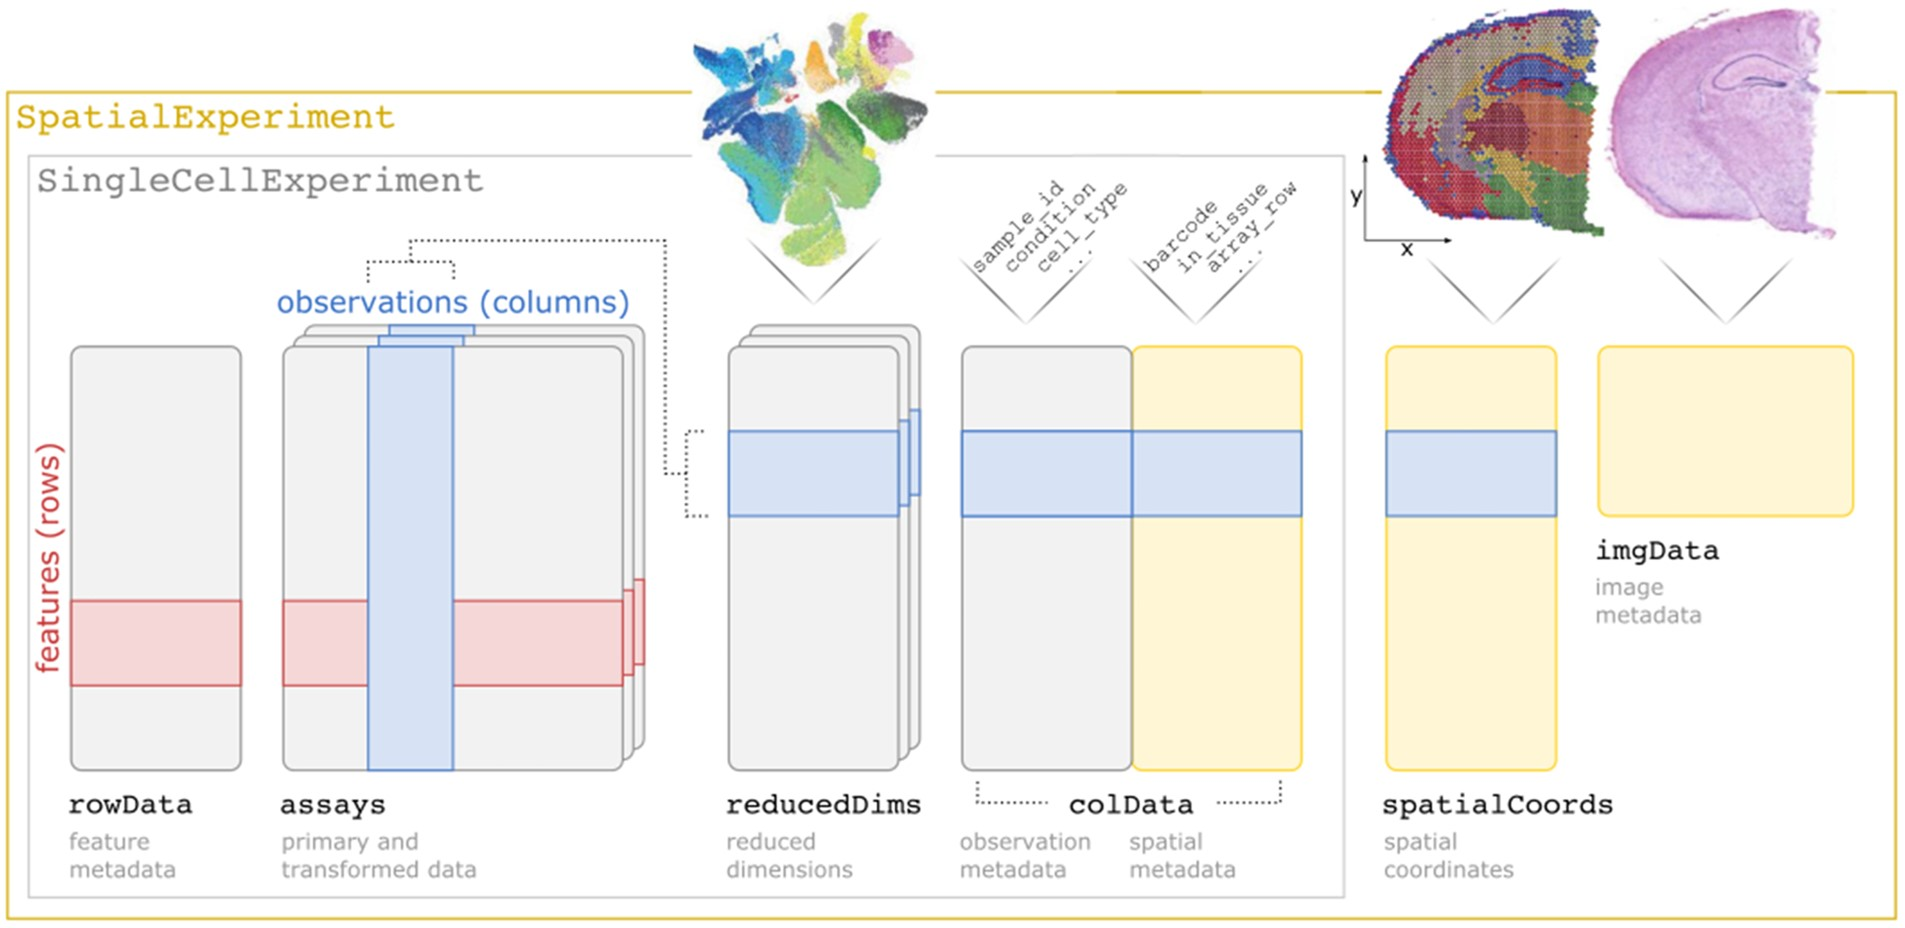
\includegraphics[width=1\linewidth]{images/SpatialExperiment} 

}

\caption{Overview of the `SpatialExperiment` object class structure.}\label{fig:SpExp-overview}
\end{figure}

For more details, see the related publication from Righelli et al., 2021 describing the \texttt{SpatialExperiment} \citep{Righelli2022Jun}.

\hypertarget{inspect-the-object}{%
\subsection{Inspect the object}\label{inspect-the-object}}

\begin{Shaded}
\begin{Highlighting}[]
\DocumentationTok{\#\# Check the object\textquotesingle{}s structure}
\NormalTok{spe}
\end{Highlighting}
\end{Shaded}

\begin{verbatim}
## class: SpatialExperiment 
## dim: 33538 4992 
## metadata(0):
## assays(1): counts
## rownames(33538): ENSG00000243485 ENSG00000237613 ... ENSG00000277475
##   ENSG00000268674
## rowData names(3): gene_id gene_name feature_type
## colnames(4992): AAACAACGAATAGTTC-1 AAACAAGTATCTCCCA-1 ...
##   TTGTTTGTATTACACG-1 TTGTTTGTGTAAATTC-1
## colData names(7): barcode_id sample_id ... ground_truth cell_count
## reducedDimNames(0):
## mainExpName: NULL
## altExpNames(0):
## spatialCoords names(2) : pxl_col_in_fullres pxl_row_in_fullres
## imgData names(4): sample_id image_id data scaleFactor
\end{verbatim}

\begin{Shaded}
\begin{Highlighting}[]
\DocumentationTok{\#\# Check number of features/genes (rows) and spots (columns)}
\FunctionTok{dim}\NormalTok{(spe)}
\end{Highlighting}
\end{Shaded}

\begin{verbatim}
## [1] 33538  4992
\end{verbatim}

\begin{Shaded}
\begin{Highlighting}[]
\DocumentationTok{\#\# Check names of \textquotesingle{}assay\textquotesingle{} tables}
\FunctionTok{assayNames}\NormalTok{(spe)}
\end{Highlighting}
\end{Shaded}

\begin{verbatim}
## [1] "counts"
\end{verbatim}

\hypertarget{counts-table-and-gene-metadata}{%
\subsection{Counts table and gene metadata}\label{counts-table-and-gene-metadata}}

\begin{Shaded}
\begin{Highlighting}[]
\DocumentationTok{\#\# Have a look at the counts table}
\FunctionTok{assay}\NormalTok{(spe)[}\DecValTok{1}\SpecialCharTok{:}\DecValTok{6}\NormalTok{,}\DecValTok{1}\SpecialCharTok{:}\DecValTok{4}\NormalTok{]}
\end{Highlighting}
\end{Shaded}

\begin{verbatim}
## 6 x 4 sparse Matrix of class "dgTMatrix"
##                 AAACAACGAATAGTTC-1 AAACAAGTATCTCCCA-1 AAACAATCTACTAGCA-1
## ENSG00000243485                  .                  .                  .
## ENSG00000237613                  .                  .                  .
## ENSG00000186092                  .                  .                  .
## ENSG00000238009                  .                  .                  .
## ENSG00000239945                  .                  .                  .
## ENSG00000239906                  .                  .                  .
##                 AAACACCAATAACTGC-1
## ENSG00000243485                  .
## ENSG00000237613                  .
## ENSG00000186092                  .
## ENSG00000238009                  .
## ENSG00000239945                  .
## ENSG00000239906                  .
\end{verbatim}

As we can see here the counts table is an object of class \texttt{dgTMatrix} which is a sparse matrix. This is because much like scRNA-seq data, STx data include many zeros. As a result, to make the counts table as light as possible we resort to using sparse matrices. This next code chunk examines a part of the matrix that includes genes with some level of expression:

\begin{Shaded}
\begin{Highlighting}[]
\FunctionTok{assay}\NormalTok{(spe)[}\DecValTok{20}\SpecialCharTok{:}\DecValTok{40}\NormalTok{, }\DecValTok{2000}\SpecialCharTok{:}\DecValTok{2010}\NormalTok{]}
\end{Highlighting}
\end{Shaded}

\begin{verbatim}
## 21 x 11 sparse Matrix of class "dgTMatrix"
##                                      
## ENSG00000223764 . . . . . . . . . . .
## ENSG00000187634 . . . . . . . . . . .
## ENSG00000188976 . . 2 . . . . . . 1 1
## ENSG00000187961 . . . . . . . . . . .
## ENSG00000187583 . . . . . . . . . . .
## ENSG00000187642 . . . . . . . . . . .
## ENSG00000272512 . . . . . . . . . . .
## ENSG00000188290 1 . . . . . . . . 2 .
## ENSG00000187608 . 1 . . . . 2 . . 1 .
## ENSG00000224969 . . . . . . . . . . .
## ENSG00000188157 . 1 . . 2 . . . . 1 .
## ENSG00000273443 . . . . . . . . . . .
## ENSG00000237330 . . . . . . . . . . .
## ENSG00000131591 . . . . . . . . . 1 .
## ENSG00000223823 . . . . . . . . . . .
## ENSG00000272141 . . . . . . . . . . .
## ENSG00000205231 . . . . . . . . . . .
## ENSG00000162571 . . . . . . . . . . .
## ENSG00000186891 . . . 1 . . . . . . .
## ENSG00000186827 . . . . . . . . . . .
## ENSG00000078808 . 1 2 . 1 . . . . 1 .
\end{verbatim}

\begin{Shaded}
\begin{Highlighting}[]
\FunctionTok{assay}\NormalTok{(spe)[}\DecValTok{33488}\SpecialCharTok{:}\DecValTok{33508}\NormalTok{, }\DecValTok{2000}\SpecialCharTok{:}\DecValTok{2010}\NormalTok{]}
\end{Highlighting}
\end{Shaded}

\begin{verbatim}
## 21 x 11 sparse Matrix of class "dgTMatrix"
##                                                     
## ENSG00000160294  .  .   .  .   .   .  .  .  .   .  .
## ENSG00000228137  .  .   .  .   .   .  .  .  .   .  .
## ENSG00000239415  .  .   .  .   .   .  .  .  .   .  .
## ENSG00000182362  .  .   .  .   .   .  .  .  1   .  .
## ENSG00000160298  .  .   .  .   .   .  .  .  .   .  .
## ENSG00000160299  .  .   1  .   1   .  .  .  .   .  .
## ENSG00000160305  .  .   .  .   .   2  .  .  .   .  .
## ENSG00000160307  1  3   1  1   4   5  1  1  .   2  1
## ENSG00000160310  .  .   .  .   1   .  .  .  .   2  .
## ENSG00000198888 17 44  71 16 154  97 12 14 32 167  6
## ENSG00000198763 16 59  64 11 116  63 11 12 18 123  6
## ENSG00000198804 37 85 155 25 252 176 24 27 38 335 12
## ENSG00000198712 23 79 120 23 214 170 22 25 48 242 10
## ENSG00000228253  2  .   3  .   1   .  .  1  1   6  .
## ENSG00000198899 20 39  93  9 136 108 20 18 25 165  7
## ENSG00000198938 27 59 133 20 216 120 22 26 43 232  9
## ENSG00000198840  5 27  33  5  71  39  8 11 12  78  .
## ENSG00000212907  2  .   4  2   7   5  .  1  1   9  .
## ENSG00000198886 15 65  95  9 183  98 18 19 33 178  7
## ENSG00000198786  2 10  10  3  20  14  1  2  2  25  4
## ENSG00000198695  1  1   3  .   2   2  .  .  .   1  .
\end{verbatim}

The levels of expression of different genes in the same spots differ significantly with many low values being present. We have to remember here that this data is not as yet normalized, and is therefore affected by systematic factors such as library size. Nonetheless, what is demonstrated here is typical for STx data (as it is for scRNA-seq data) - many genes will show low expression in individual spots.

To continue our exploration of the information stored in the \texttt{SpatialExperiment} object:

\begin{Shaded}
\begin{Highlighting}[]
\DocumentationTok{\#\# Have a look at the genes metadata}
\FunctionTok{head}\NormalTok{(}\FunctionTok{rowData}\NormalTok{(spe))}
\end{Highlighting}
\end{Shaded}

\begin{verbatim}
## DataFrame with 6 rows and 3 columns
##                         gene_id   gene_name    feature_type
##                     <character> <character>     <character>
## ENSG00000243485 ENSG00000243485 MIR1302-2HG Gene Expression
## ENSG00000237613 ENSG00000237613     FAM138A Gene Expression
## ENSG00000186092 ENSG00000186092       OR4F5 Gene Expression
## ENSG00000238009 ENSG00000238009  AL627309.1 Gene Expression
## ENSG00000239945 ENSG00000239945  AL627309.3 Gene Expression
## ENSG00000239906 ENSG00000239906  AL627309.2 Gene Expression
\end{verbatim}

\hypertarget{coordinates-table-and-spot-metadata}{%
\subsection{Coordinates table and spot metadata}\label{coordinates-table-and-spot-metadata}}

The data that distinguished a \texttt{SpatialExperiment} object is the coordinate data which describes the spatial location of each spot.

\begin{Shaded}
\begin{Highlighting}[]
\DocumentationTok{\#\# Check the spatial coordinates}
\FunctionTok{head}\NormalTok{(}\FunctionTok{spatialCoords}\NormalTok{(spe))}
\end{Highlighting}
\end{Shaded}

\begin{verbatim}
##                    pxl_col_in_fullres pxl_row_in_fullres
## AAACAACGAATAGTTC-1               3913               2435
## AAACAAGTATCTCCCA-1               9791               8468
## AAACAATCTACTAGCA-1               5769               2807
## AAACACCAATAACTGC-1               4068               9505
## AAACAGAGCGACTCCT-1               9271               4151
## AAACAGCTTTCAGAAG-1               3393               7583
\end{verbatim}

\begin{Shaded}
\begin{Highlighting}[]
\DocumentationTok{\#\# spot{-}level metadata}
\FunctionTok{head}\NormalTok{(}\FunctionTok{colData}\NormalTok{(spe))}
\end{Highlighting}
\end{Shaded}

\begin{verbatim}
## DataFrame with 6 rows and 7 columns
##                            barcode_id     sample_id in_tissue array_row
##                           <character>   <character> <integer> <integer>
## AAACAACGAATAGTTC-1 AAACAACGAATAGTTC-1 sample_151673         0         0
## AAACAAGTATCTCCCA-1 AAACAAGTATCTCCCA-1 sample_151673         1        50
## AAACAATCTACTAGCA-1 AAACAATCTACTAGCA-1 sample_151673         1         3
## AAACACCAATAACTGC-1 AAACACCAATAACTGC-1 sample_151673         1        59
## AAACAGAGCGACTCCT-1 AAACAGAGCGACTCCT-1 sample_151673         1        14
## AAACAGCTTTCAGAAG-1 AAACAGCTTTCAGAAG-1 sample_151673         1        43
##                    array_col ground_truth cell_count
##                    <integer>  <character>  <integer>
## AAACAACGAATAGTTC-1        16           NA         NA
## AAACAAGTATCTCCCA-1       102       Layer3          6
## AAACAATCTACTAGCA-1        43       Layer1         16
## AAACACCAATAACTGC-1        19           WM          5
## AAACAGAGCGACTCCT-1        94       Layer3          2
## AAACAGCTTTCAGAAG-1         9       Layer5          4
\end{verbatim}

\hypertarget{image-metadata}{%
\subsection{Image metadata}\label{image-metadata}}

Finally, the \texttt{SpatialExperiment} object also contains the image data from the STx experiment, giving the coordinates we looked at in the previous section some context in terms of the tissue of origin.

\begin{Shaded}
\begin{Highlighting}[]
\DocumentationTok{\#\# Have a look at the image metadata}
\FunctionTok{imgData}\NormalTok{(spe)}
\end{Highlighting}
\end{Shaded}

\begin{verbatim}
## DataFrame with 2 rows and 4 columns
##       sample_id    image_id   data scaleFactor
##     <character> <character> <list>   <numeric>
## 1 sample_151673      lowres   ####   0.0450045
## 2 sample_151673       hires   ####   0.1500150
\end{verbatim}

As well as this (fairly basic) metadata, the \texttt{spe} object also contains the image itself, which the \texttt{SpatialExperiment} class allows us to access, like so:

\begin{Shaded}
\begin{Highlighting}[]
\DocumentationTok{\#\# retrieve the image}
\NormalTok{spi }\OtherTok{\textless{}{-}} \FunctionTok{getImg}\NormalTok{(spe)}
\DocumentationTok{\#\# "plot" the image}
\FunctionTok{plot}\NormalTok{(}\FunctionTok{imgRaster}\NormalTok{(spi))}
\end{Highlighting}
\end{Shaded}

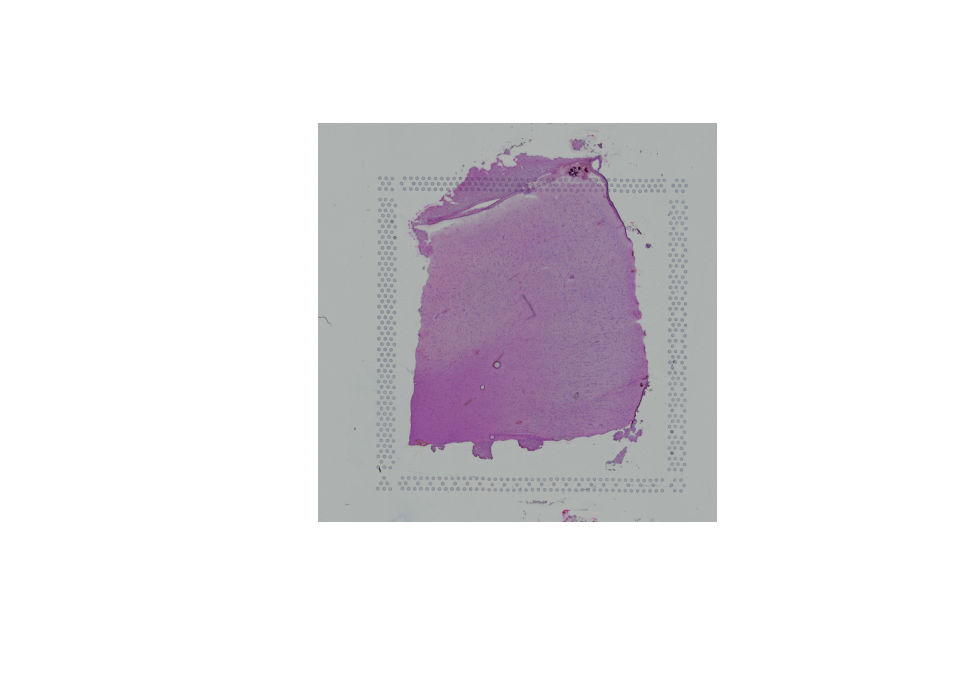
\includegraphics{_main_files/figure-latex/01_plot-image-1.pdf}

We can also use the scaling factors in the \texttt{imgData} to plot the locations of the Visium spots over the image. The position of a point in an image does not map directly to the spot location in cartesian coordinates, as it is the top-left of an image that is (0,0), not the bottom-left. In order to manage this, we need to transform the y-axis coordinates.

\begin{Shaded}
\begin{Highlighting}[]
\DocumentationTok{\#\# "Plot" the image}
\FunctionTok{plot}\NormalTok{(}\FunctionTok{imgRaster}\NormalTok{(spi))}
\DocumentationTok{\#\# Extract the spot locations}
\NormalTok{spot\_coords }\OtherTok{\textless{}{-}} \FunctionTok{spatialCoords}\NormalTok{(spe) }\SpecialCharTok{\%\textgreater{}\%}\NormalTok{ as.data.frame}
\DocumentationTok{\#\# Scale by low{-}res factor}
\NormalTok{lowres\_scale }\OtherTok{\textless{}{-}} \FunctionTok{imgData}\NormalTok{(spe)[}\FunctionTok{imgData}\NormalTok{(spe)}\SpecialCharTok{$}\NormalTok{image\_id }\SpecialCharTok{==} \StringTok{\textquotesingle{}lowres\textquotesingle{}}\NormalTok{, }\StringTok{\textquotesingle{}scaleFactor\textquotesingle{}}\NormalTok{]}
\NormalTok{spot\_coords}\SpecialCharTok{$}\NormalTok{x\_axis }\OtherTok{\textless{}{-}}\NormalTok{ spot\_coords}\SpecialCharTok{$}\NormalTok{pxl\_col\_in\_fullres }\SpecialCharTok{*}\NormalTok{ lowres\_scale}
\NormalTok{spot\_coords}\SpecialCharTok{$}\NormalTok{y\_axis }\OtherTok{\textless{}{-}}\NormalTok{ spot\_coords}\SpecialCharTok{$}\NormalTok{pxl\_row\_in\_fullres }\SpecialCharTok{*}\NormalTok{ lowres\_scale}
\DocumentationTok{\#\# lowres image is 600x600 pixels}
\FunctionTok{dim}\NormalTok{(}\FunctionTok{imgRaster}\NormalTok{(spi))}
\end{Highlighting}
\end{Shaded}

\begin{verbatim}
## [1] 600 600
\end{verbatim}

\begin{Shaded}
\begin{Highlighting}[]
\DocumentationTok{\#\# flip the Y axis}
\NormalTok{spot\_coords}\SpecialCharTok{$}\NormalTok{y\_axis }\OtherTok{\textless{}{-}} \FunctionTok{abs}\NormalTok{(spot\_coords}\SpecialCharTok{$}\NormalTok{y\_axis }\SpecialCharTok{{-}}\NormalTok{ (}\FunctionTok{ncol}\NormalTok{(}\FunctionTok{imgRaster}\NormalTok{(spi)) }\SpecialCharTok{+} \DecValTok{1}\NormalTok{))}
\FunctionTok{points}\NormalTok{(}\AttributeTok{x=}\NormalTok{spot\_coords}\SpecialCharTok{$}\NormalTok{x\_axis, }\AttributeTok{y=}\NormalTok{spot\_coords}\SpecialCharTok{$}\NormalTok{y\_axis)}
\end{Highlighting}
\end{Shaded}

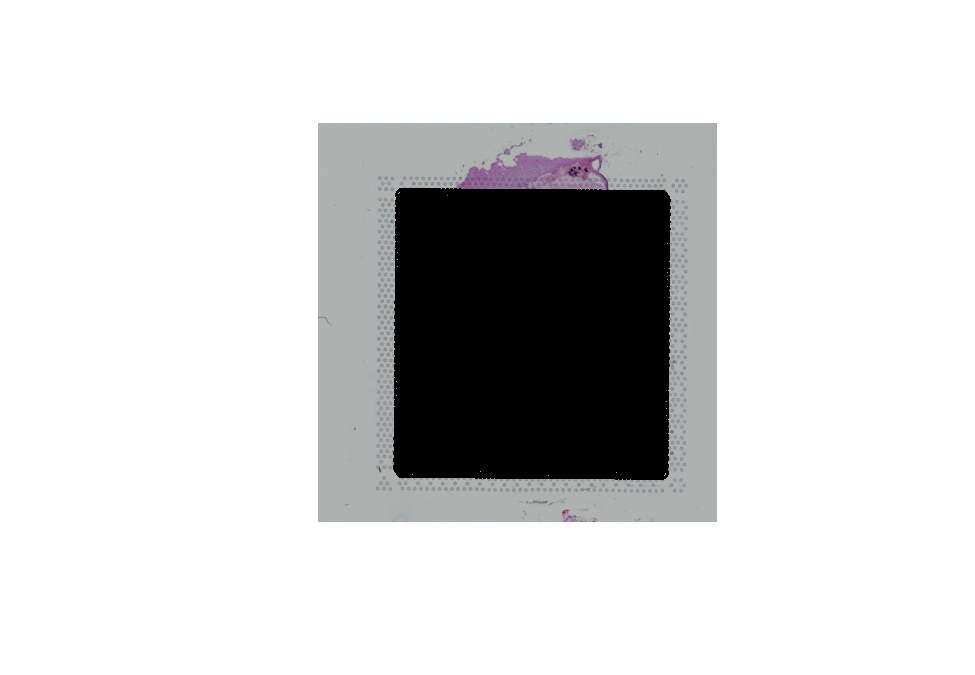
\includegraphics{_main_files/figure-latex/01_plot-spots-1.pdf}

An equivalent plot, using \texttt{ggplot2} as the plotting library:

\begin{Shaded}
\begin{Highlighting}[]
\FunctionTok{ggplot}\NormalTok{(}\AttributeTok{mapping =} \FunctionTok{aes}\NormalTok{(}\DecValTok{1}\SpecialCharTok{:}\DecValTok{600}\NormalTok{, }\DecValTok{1}\SpecialCharTok{:}\DecValTok{600}\NormalTok{)) }\SpecialCharTok{+}
  \FunctionTok{annotation\_raster}\NormalTok{(}\FunctionTok{imgRaster}\NormalTok{(spi), }\AttributeTok{xmin =} \DecValTok{1}\NormalTok{, }\AttributeTok{xmax =} \DecValTok{600}\NormalTok{, }\AttributeTok{ymin =} \DecValTok{1}\NormalTok{, }\AttributeTok{ymax =} \DecValTok{600}\NormalTok{) }\SpecialCharTok{+}
  \FunctionTok{geom\_point}\NormalTok{(}\AttributeTok{data=}\NormalTok{spot\_coords, }\FunctionTok{aes}\NormalTok{(}\AttributeTok{x=}\NormalTok{x\_axis, }\AttributeTok{y=}\NormalTok{y\_axis), }\AttributeTok{alpha=}\FloatTok{0.2}\NormalTok{) }\SpecialCharTok{+} \FunctionTok{xlim}\NormalTok{(}\DecValTok{1}\NormalTok{, }\DecValTok{600}\NormalTok{) }\SpecialCharTok{+} \FunctionTok{ylim}\NormalTok{(}\DecValTok{1}\NormalTok{, }\DecValTok{600}\NormalTok{) }\SpecialCharTok{+}
  \FunctionTok{coord\_fixed}\NormalTok{() }\SpecialCharTok{+} 
  \FunctionTok{theme\_void}\NormalTok{()}
\end{Highlighting}
\end{Shaded}

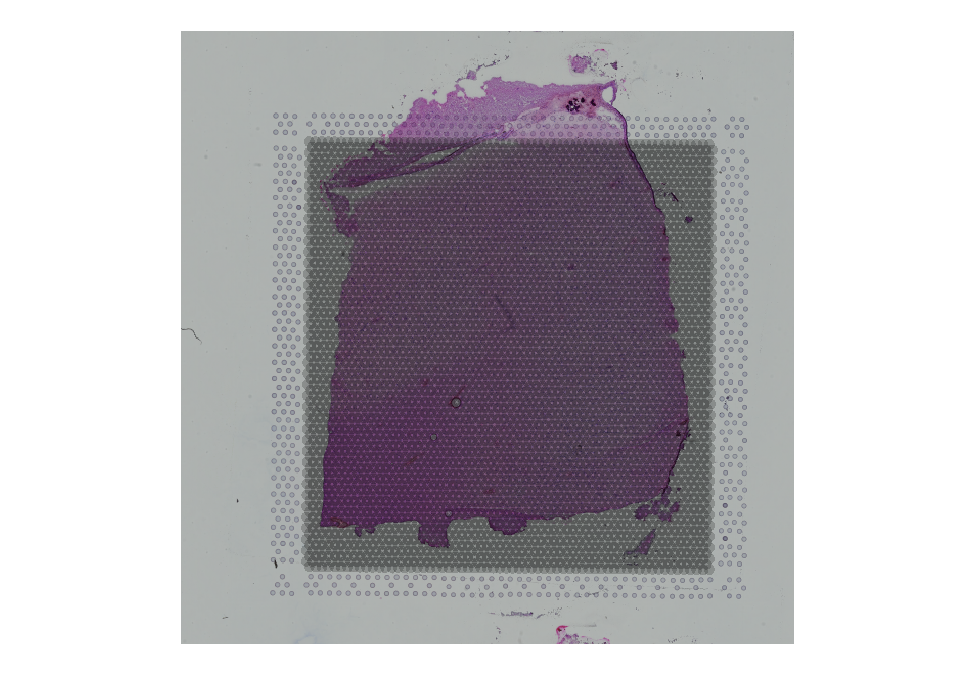
\includegraphics{_main_files/figure-latex/01_ggplot-spots-1.pdf}
We can also extract additional metadata to make these plots more informative - for instance, the annotation from \texttt{colData} that flags whether a spot is ``on tissue'' or not can be used to colour the spots like so:

\begin{Shaded}
\begin{Highlighting}[]
\DocumentationTok{\#\# Add the annotation to the coordinate data frame}
\NormalTok{spot\_coords}\SpecialCharTok{$}\NormalTok{on\_tissue }\OtherTok{\textless{}{-}} \FunctionTok{as.logical}\NormalTok{(}\FunctionTok{colData}\NormalTok{(spe)}\SpecialCharTok{$}\NormalTok{in\_tissue)}

\FunctionTok{ggplot}\NormalTok{(}\AttributeTok{mapping =} \FunctionTok{aes}\NormalTok{(}\DecValTok{1}\SpecialCharTok{:}\DecValTok{600}\NormalTok{, }\DecValTok{1}\SpecialCharTok{:}\DecValTok{600}\NormalTok{)) }\SpecialCharTok{+}
  \FunctionTok{annotation\_raster}\NormalTok{(}\FunctionTok{imgRaster}\NormalTok{(spi), }\AttributeTok{xmin =} \DecValTok{1}\NormalTok{, }\AttributeTok{xmax =} \DecValTok{600}\NormalTok{, }\AttributeTok{ymin =} \DecValTok{1}\NormalTok{, }\AttributeTok{ymax =} \DecValTok{600}\NormalTok{) }\SpecialCharTok{+}
  \FunctionTok{geom\_point}\NormalTok{(}\AttributeTok{data=}\NormalTok{spot\_coords, }\FunctionTok{aes}\NormalTok{(}\AttributeTok{x=}\NormalTok{x\_axis, }\AttributeTok{y=}\NormalTok{y\_axis, }\AttributeTok{colour=}\NormalTok{on\_tissue), }\AttributeTok{alpha=}\FloatTok{0.2}\NormalTok{) }\SpecialCharTok{+} \FunctionTok{xlim}\NormalTok{(}\DecValTok{1}\NormalTok{, }\DecValTok{600}\NormalTok{) }\SpecialCharTok{+} \FunctionTok{ylim}\NormalTok{(}\DecValTok{1}\NormalTok{, }\DecValTok{600}\NormalTok{) }\SpecialCharTok{+}
  \FunctionTok{coord\_fixed}\NormalTok{() }\SpecialCharTok{+} 
  \FunctionTok{theme\_void}\NormalTok{()}
\end{Highlighting}
\end{Shaded}

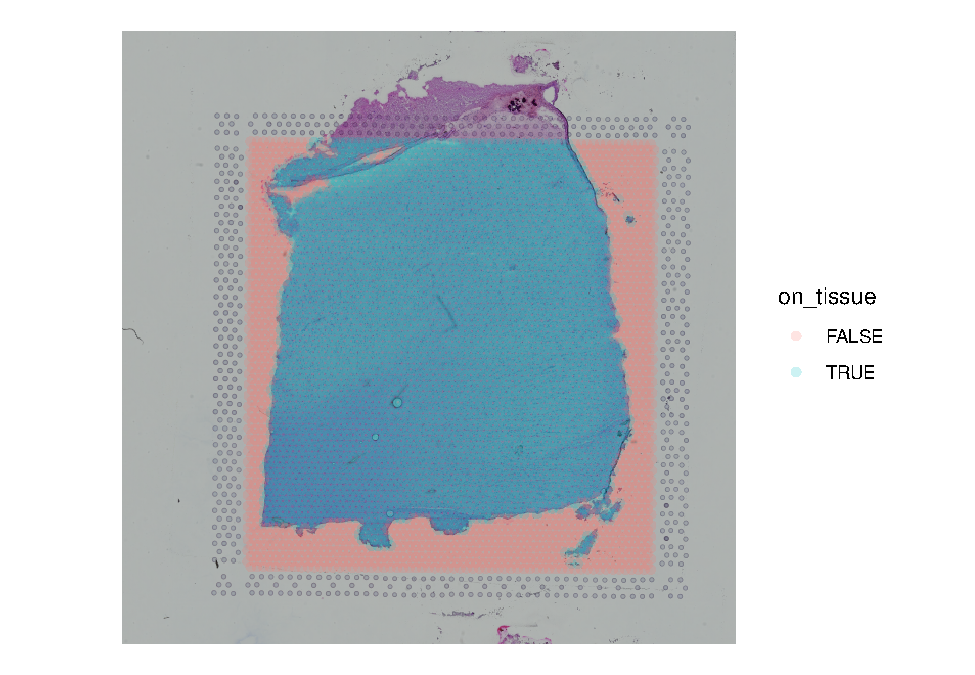
\includegraphics{_main_files/figure-latex/01_ggplot_ontissue-1.pdf}

Having to manually extract the relevant information from the \texttt{SpatialExperiment} object to generate plots like this does not generally make sense, and defies the point of using a data class that can encapsulate this information. We can instead use a package like \texttt{ggspavis}, which is explicitly built for generating visualisations of STx data directly from the \texttt{SpatialExperiment} object. We will make extensive use of this package during the next tutorial as we work through quality control processes for STx data. The pre-built nature of these plots is convenient, though it prevents users from achieving tasks like adding the tissue image to the plot. For many users the convenience will outweigh any issues this presents, though it is worth being aware of how to build visualisations from the ground up.

\begin{Shaded}
\begin{Highlighting}[]
\FunctionTok{plotSpots}\NormalTok{(spe, }\AttributeTok{in\_tissue =} \ConstantTok{NULL}\NormalTok{, }\AttributeTok{annotate=}\StringTok{\textquotesingle{}in\_tissue\textquotesingle{}}\NormalTok{, }\AttributeTok{size=}\FloatTok{0.5}\NormalTok{)}
\end{Highlighting}
\end{Shaded}

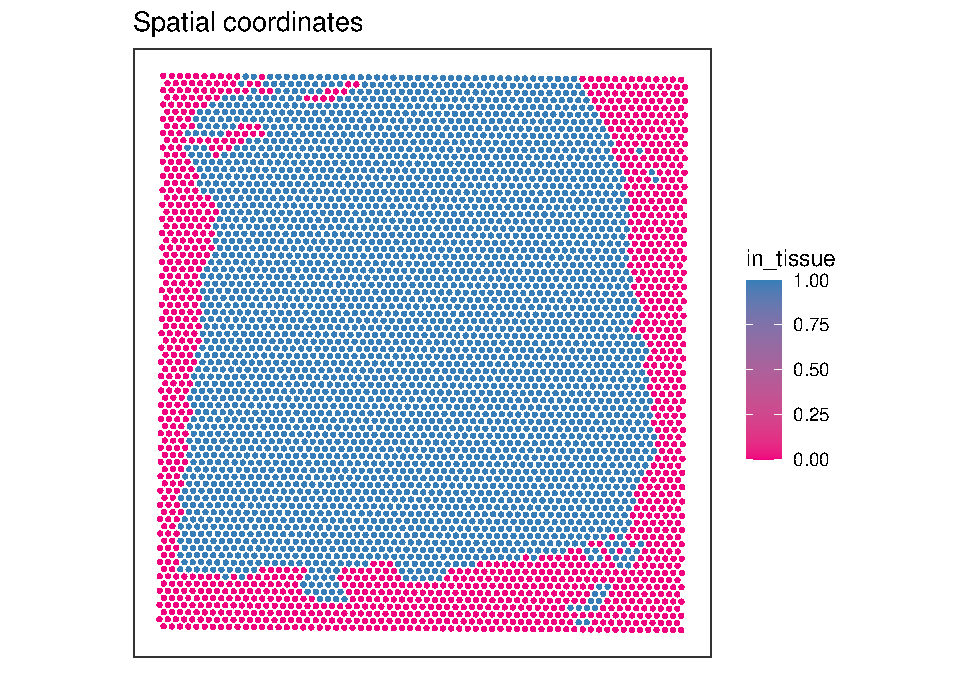
\includegraphics{_main_files/figure-latex/01_ggspavis-ontissue-1.pdf}

\hypertarget{conclusion}{%
\section{Conclusion}\label{conclusion}}

This first practical session has been a pretty straight-forward examination of an example Visium dataset. We've demonstrated where in this object the data and metadata are stored, how to extract it and make simple use of it.

\hypertarget{practical-session-2}{%
\chapter{Practical session 2}\label{practical-session-2}}

Having previously introduced some of the Bioconductor ecosystem for storing and manipulating STx data, in this second session we will focus on some of the most common STx analysis tasks - particularly quality control assessment and associated spot- and gene- level filtering. We will also consider some global methods of STx analysis, including dimensionality reduction and clustering. All of the methods demonstrated here continue to focus on interoperable packages available via Bioconductor.

\begin{Shaded}
\begin{Highlighting}[]
\DocumentationTok{\#\# Load packages \{{-}\}}
\FunctionTok{library}\NormalTok{(SpatialExperiment)}
\FunctionTok{library}\NormalTok{(STexampleData)}
\FunctionTok{library}\NormalTok{(ggspavis)}
\FunctionTok{library}\NormalTok{(ggplot2)}
\FunctionTok{library}\NormalTok{(scater)}
\FunctionTok{library}\NormalTok{(scran)}
\FunctionTok{library}\NormalTok{(igraph)}
\FunctionTok{library}\NormalTok{(pheatmap)}
\FunctionTok{library}\NormalTok{(ggExtra)}
\end{Highlighting}
\end{Shaded}

\begin{itemize}
\item
  \href{https://bioconductor.org/packages/release/bioc/html/ggspavis.html}{\texttt{ggspavis}} is a Bioconductor package that includes visualization functions for spatially resolved transcriptomics datasets stored in \texttt{SpatialExperiment} format from spot-based (e.g., 10x Genomics Visium) platforms (\citet{ggspavis2023Apr}).
\item
  \href{https://bioconductor.org/packages/release/bioc/html/scater.html}{\texttt{scater}} is also a Bioconductor package that is a selection of tools for doing various analyses of scRNA-seq gene expression data, with a focus on quality control and visualization which has extended applications to STx data too. It is based on the \texttt{SingleCellExperiment} and \texttt{SpatialExperiment} classes and thus is interoperable with many other Bioconductor packages such as \href{Spot-level\%20quality\%20control\%20(sQC)\%20procedures\%20are\%20employed\%20to\%20eliminate\%20low-quality\%20spots\%20before\%20conducting\%20further\%20analyses}{\texttt{scran}}, \href{https://bioconductor.org/packages/release/scuttle}{\texttt{scuttle}} and \href{https://bioconductor.org/packages/release/iSEE}{\texttt{iSEE}}.
\end{itemize}

\begin{Shaded}
\begin{Highlighting}[]
\DocumentationTok{\#\# Reload the example dataset}
\NormalTok{spe }\OtherTok{\textless{}{-}} \FunctionTok{Visium\_humanDLPFC}\NormalTok{()}
\end{Highlighting}
\end{Shaded}

\begin{verbatim}
## see ?STexampleData and browseVignettes('STexampleData') for documentation
\end{verbatim}

\begin{verbatim}
## loading from cache
\end{verbatim}

\hypertarget{spot-level-quality-control}{%
\section{Spot-level Quality Control}\label{spot-level-quality-control}}

Considered quality control (QC) procedures are essential for analysing any high-throughput data in molecular biology. The removal of noise and low quality data from complex datasets can improve the reliability of downsrtream analyses. STx is no different in this regard, and QC can be undertaken in 2 main places - spot-level and gene-level. Here, we focus on spot-level QC.

Spot-level quality control (sQC) procedures are employed to eliminate low-quality spots before conducting further analyses. Low-quality spots may result from issues during library preparation or other experimental procedures, such as a high percentage of dead cells due to cell damage during library preparation, or low mRNA capture efficiency caused by ineffective reverse transcription or PCR amplification. Keeping these spots usually leads to creating problems during downstream analyses.

We can identify low-quality spots using several characteristics that are also used in cell-level QC for scRNA-sq data, including:

\begin{enumerate}
\def\labelenumi{\arabic{enumi}.}
\tightlist
\item
  \textbf{library size} (total of UMI counts per spot will vary due to sequencing \emph{-like different samples in a bulk RNA-seq-}, or due to number of cells in the spot)
\item
  \textbf{number of expressed genes} (i.e.~number of genes with non-zero UMI counts per spot)
\item
  \textbf{proportion of reads mapping to mitochondrial genes} (a high proportion indicates putative cell damage)
\end{enumerate}

Low library size or low number of expressed features can indicate poor mRNA capture rates, e.g.~due to cell damage and missing mRNAs, or low reaction efficiency. A high proportion of mitochondrial reads indicates cell damage, e.g.~partial cell lysis leading to leakage and missing cytoplasmic mRNAs, with the resulting reads therefore concentrated on the remaining mitochondrial mRNAs that are relatively protected inside the mitochondrial membrane. Unusually high numbers of cells per spot can indicate problems during cell segmentation.

The idea of using scRNA-seq QC metrics in STx data comes from the fact that if we remove space and effectively treat each spot as a single cell, the two datasets share common features. We need to bear in mind, however, that the expected distributions for high-quality \emph{spots} are different (compared to high-quality \emph{cells} in scRNA-seq), since spots may contain zero, one, or multiple cells.

A few publications for further reading that can help you understand the quality controls: \citet{McCarthy2017Apr} and \citet{Amezquita2020Feb}.

\hypertarget{plot-tissue-map}{%
\subsection{Plot tissue map}\label{plot-tissue-map}}

The dorso-lateral prefrontal cortex (DLPFC) is a functional brain region in primates involved in executive function. It consists of six layers of neurons that differ in their cell types, density and connections. The DLPFC dataset we looked at in session one, and will be here using comes with manual annotation of these layers (and the adjacent white matter - WM) by the authors \citet{Maynard2021Mar}. We can plot the tissue map with and without the annotations to get a complete view.

\begin{Shaded}
\begin{Highlighting}[]
\DocumentationTok{\#\# Plot spatial coordinates without annotations}
\FunctionTok{plotSpots}\NormalTok{(spe)}

\DocumentationTok{\#\# Plot spatial coordinates with annotations}
\FunctionTok{plotSpots}\NormalTok{(spe,}
          \AttributeTok{annotate =} \StringTok{"ground\_truth"}\NormalTok{)}
\end{Highlighting}
\end{Shaded}

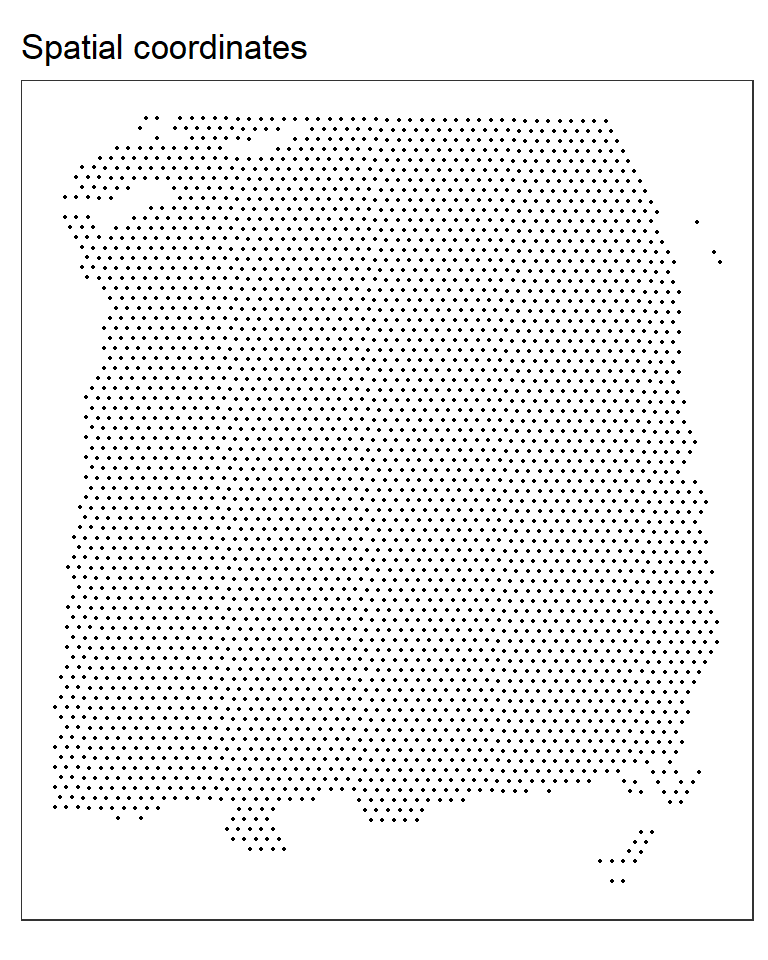
\includegraphics[width=0.5\linewidth]{_main_files/figure-latex/02_plot-maps-gTruth-1} 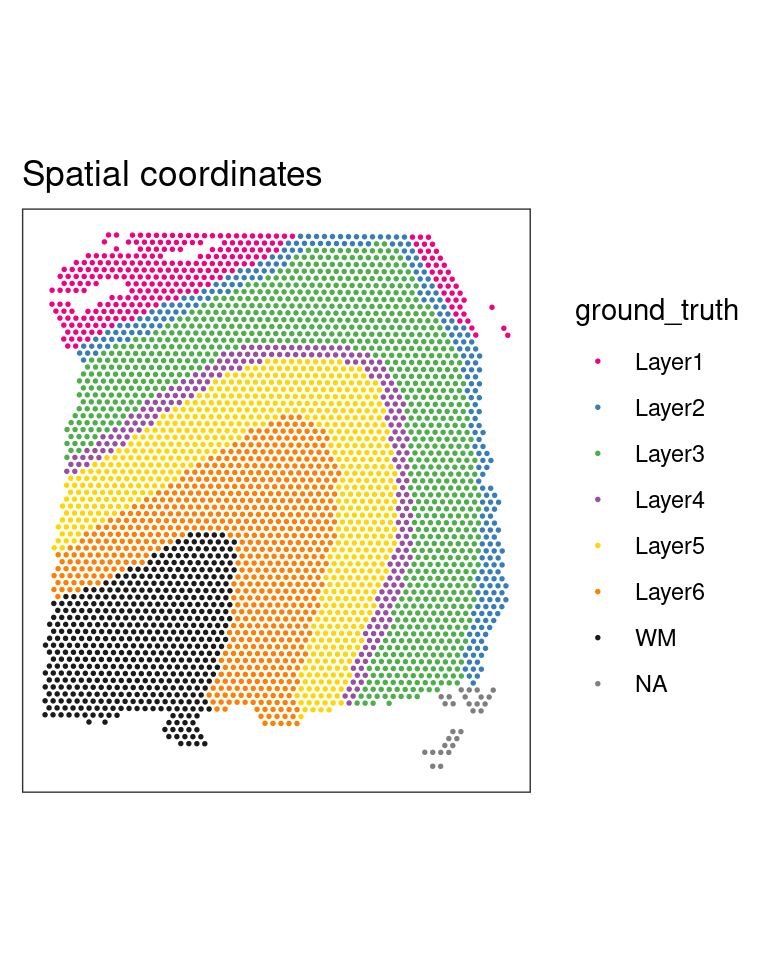
\includegraphics[width=0.5\linewidth]{_main_files/figure-latex/02_plot-maps-gTruth-2}

\hypertarget{calculating-qc-metrics}{%
\subsection{Calculating QC metrics}\label{calculating-qc-metrics}}

We will calculate the three main QC metrics described above using methods from the \texttt{scater} \citep{McCarthy2017Apr} package, and investigate their influence on the DLPFC dataset with some plots from \texttt{ggspavis}, along with some additional plots of our own.

At present, the dataset contains both on- and off-tissue spots - we plotted these in the previous practical. For any future analysis though we are only interested in the on-tissue spots. Therefore, before we run any calculations we want to remove the off-tissue spots.

\textbf{\emph{NOTE}}: the on- or off-tissue information for each spot can be found in the \texttt{colData} of the \texttt{spe} object and in the \texttt{in\_tissue} column where \emph{0 = off-tissue} and \emph{1 = on-tissue}.

\begin{Shaded}
\begin{Highlighting}[]
\DocumentationTok{\#\# Dataset dimensions before the filtering}
\FunctionTok{dim}\NormalTok{(spe)}
\end{Highlighting}
\end{Shaded}

\begin{verbatim}
## [1] 33538  4992
\end{verbatim}

\begin{Shaded}
\begin{Highlighting}[]
\DocumentationTok{\#\# Subset to keep only on{-}tissue spots}
\NormalTok{spe }\OtherTok{\textless{}{-}}\NormalTok{ spe[, }\FunctionTok{colData}\NormalTok{(spe)}\SpecialCharTok{$}\NormalTok{in\_tissue }\SpecialCharTok{==} \DecValTok{1}\NormalTok{]}
\FunctionTok{dim}\NormalTok{(spe)}
\end{Highlighting}
\end{Shaded}

\begin{verbatim}
## [1] 33538  3639
\end{verbatim}

The next thing we need to do before we make decisions on how to quality \emph{``trim''} the dataset is to calculate the percentage per spot of mitochodrial gene expression and store this information inside the \texttt{colData}. First of all, find the mitochrondrial genes - their gene names start with ``MT-'' or ``mt-''.

\begin{Shaded}
\begin{Highlighting}[]
\DocumentationTok{\#\# Classify genes as "mitochondrial" (is\_mito == TRUE) }
\DocumentationTok{\#\# or not (is\_mito == FALSE)}
\NormalTok{is\_mito }\OtherTok{\textless{}{-}} \FunctionTok{grepl}\NormalTok{(}\StringTok{"(\^{}MT{-})|(\^{}mt{-})"}\NormalTok{, }\FunctionTok{rowData}\NormalTok{(spe)}\SpecialCharTok{$}\NormalTok{gene\_name)}
\FunctionTok{rowData}\NormalTok{(spe)}\SpecialCharTok{$}\NormalTok{gene\_name[is\_mito]}
\end{Highlighting}
\end{Shaded}

\begin{verbatim}
##  [1] "MT-ND1"  "MT-ND2"  "MT-CO1"  "MT-CO2"  "MT-ATP8" "MT-ATP6" "MT-CO3" 
##  [8] "MT-ND3"  "MT-ND4L" "MT-ND4"  "MT-ND5"  "MT-ND6"  "MT-CYB"
\end{verbatim}

Then find what proportion of reads in a spot's library are attributable to the expression of these genes. This uses a function, \texttt{addPerCellQC()} from \texttt{scater} (which in this instance is actually a wrapper around \texttt{scuttle}).

\begin{Shaded}
\begin{Highlighting}[]
\DocumentationTok{\#\# Calculate per{-}spot QC metrics and store in colData}
\NormalTok{spe }\OtherTok{\textless{}{-}} \FunctionTok{addPerCellQC}\NormalTok{(spe, }\AttributeTok{subsets =} \FunctionTok{list}\NormalTok{(}\AttributeTok{mito =}\NormalTok{ is\_mito))}
\FunctionTok{head}\NormalTok{(}\FunctionTok{colData}\NormalTok{(spe))}
\end{Highlighting}
\end{Shaded}

\begin{verbatim}
## DataFrame with 6 rows and 13 columns
##                            barcode_id     sample_id in_tissue array_row
##                           <character>   <character> <integer> <integer>
## AAACAAGTATCTCCCA-1 AAACAAGTATCTCCCA-1 sample_151673         1        50
## AAACAATCTACTAGCA-1 AAACAATCTACTAGCA-1 sample_151673         1         3
## AAACACCAATAACTGC-1 AAACACCAATAACTGC-1 sample_151673         1        59
## AAACAGAGCGACTCCT-1 AAACAGAGCGACTCCT-1 sample_151673         1        14
## AAACAGCTTTCAGAAG-1 AAACAGCTTTCAGAAG-1 sample_151673         1        43
## AAACAGGGTCTATATT-1 AAACAGGGTCTATATT-1 sample_151673         1        47
##                    array_col ground_truth cell_count       sum  detected
##                    <integer>  <character>  <integer> <numeric> <numeric>
## AAACAAGTATCTCCCA-1       102       Layer3          6      8458      3586
## AAACAATCTACTAGCA-1        43       Layer1         16      1667      1150
## AAACACCAATAACTGC-1        19           WM          5      3769      1960
## AAACAGAGCGACTCCT-1        94       Layer3          2      5433      2424
## AAACAGCTTTCAGAAG-1         9       Layer5          4      4278      2264
## AAACAGGGTCTATATT-1        13       Layer6          6      4004      2178
##                    subsets_mito_sum subsets_mito_detected subsets_mito_percent
##                           <numeric>             <numeric>            <numeric>
## AAACAAGTATCTCCCA-1             1407                    13              16.6351
## AAACAATCTACTAGCA-1              204                    11              12.2376
## AAACACCAATAACTGC-1              430                    13              11.4089
## AAACAGAGCGACTCCT-1             1316                    13              24.2223
## AAACAGCTTTCAGAAG-1              651                    12              15.2174
## AAACAGGGTCTATATT-1              621                    13              15.5095
##                        total
##                    <numeric>
## AAACAAGTATCTCCCA-1      8458
## AAACAATCTACTAGCA-1      1667
## AAACACCAATAACTGC-1      3769
## AAACAGAGCGACTCCT-1      5433
## AAACAGCTTTCAGAAG-1      4278
## AAACAGGGTCTATATT-1      4004
\end{verbatim}

After calculating a required metric, we need to apply a cut-off threshold for the metric to decide whether or not to keep each spot. It is important to consider an individual dataset on its own merits, as it might need slightly different cut-off values to be applied. As a result we cannot rely on identifying a single value to use every time and we need to rely on plotting these metrics and making a decision on a dataset-by-dataset basis.

\hypertarget{library-size-threshold-plot}{%
\subsection{Library size threshold plot}\label{library-size-threshold-plot}}

We can plot a histogram of the library sizes across spots. The library size is the number of UMI counts in each spot. We can find this information in the \texttt{sum} column in the \texttt{colData}.

\begin{Shaded}
\begin{Highlighting}[]
\DocumentationTok{\#\# Density and histogram of library sizes}
\FunctionTok{ggplot}\NormalTok{(}\AttributeTok{data =} \FunctionTok{as.data.frame}\NormalTok{(}\FunctionTok{colData}\NormalTok{(spe)),}
       \FunctionTok{aes}\NormalTok{(}\AttributeTok{x =}\NormalTok{ sum)) }\SpecialCharTok{+}
  \FunctionTok{geom\_histogram}\NormalTok{(}\FunctionTok{aes}\NormalTok{(}\AttributeTok{y =} \FunctionTok{after\_stat}\NormalTok{(density)), }
                 \AttributeTok{colour =} \StringTok{"black"}\NormalTok{, }
                 \AttributeTok{fill =} \StringTok{"grey"}\NormalTok{) }\SpecialCharTok{+}
  \FunctionTok{geom\_density}\NormalTok{(}\AttributeTok{alpha =} \FloatTok{0.5}\NormalTok{,}
               \AttributeTok{adjust =} \FloatTok{1.0}\NormalTok{,}
               \AttributeTok{fill =} \StringTok{"\#A0CBE8"}\NormalTok{,}
               \AttributeTok{colour =} \StringTok{"\#4E79A7"}\NormalTok{) }\SpecialCharTok{+}
  \FunctionTok{scale\_x\_continuous}\NormalTok{(}\AttributeTok{breaks =}\NormalTok{ scales}\SpecialCharTok{::}\FunctionTok{pretty\_breaks}\NormalTok{(}\AttributeTok{n =} \DecValTok{10}\NormalTok{)) }\SpecialCharTok{+} 
  \FunctionTok{scale\_y\_continuous}\NormalTok{(}\AttributeTok{breaks =}\NormalTok{ scales}\SpecialCharTok{::}\FunctionTok{pretty\_breaks}\NormalTok{(}\AttributeTok{n =} \DecValTok{10}\NormalTok{)) }\SpecialCharTok{+} 
  \FunctionTok{xlab}\NormalTok{(}\StringTok{"Library size"}\NormalTok{) }\SpecialCharTok{+} 
  \FunctionTok{ylab}\NormalTok{(}\StringTok{"Density"}\NormalTok{) }\SpecialCharTok{+} 
  \FunctionTok{theme\_classic}\NormalTok{()}
\end{Highlighting}
\end{Shaded}

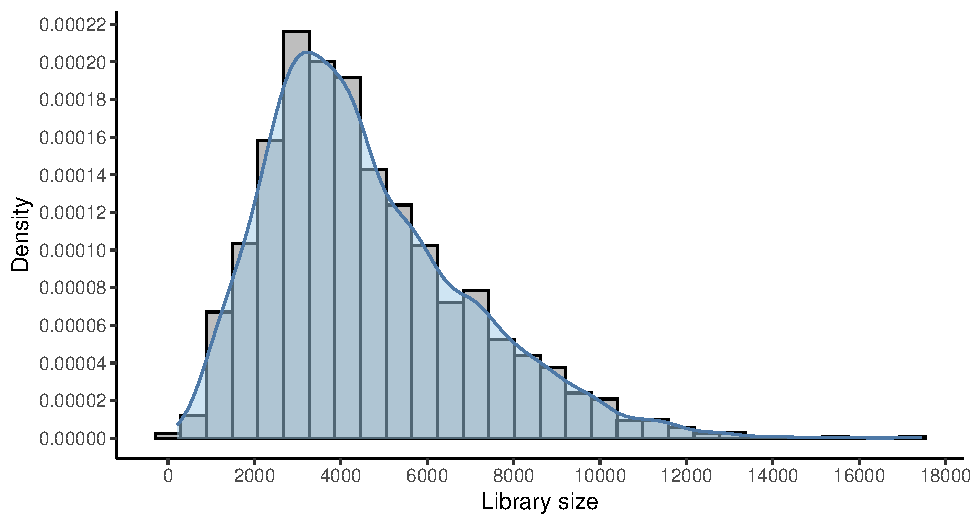
\includegraphics{_main_files/figure-latex/02_plot-libSize-histo-1.pdf}

As we can see there are no obvious issues with the library sizes. An example of an issue could be a high frequency of small libraries which would indicate poor experimental output. Generally we do not want to keep spots with too small libraries.

If the dataset we are analysing contains the number of cells that are present in each spot (this one does), then it makes sense to also plot the library sizes against the number of cells per spot. In that way we are making sure that we don't remove any spots that may have biological meaning. In many cases though the datasets do not have such information unless we can generate it using a nuclei segmentation tool to extract this information from the H\&E images.

The horizontal red line (argument \texttt{threshold} in the \texttt{plotQC} function) shows a first guess at a possible filtering threshold for library size based on the above histogram.

NOTE: The \texttt{ggspavis} plots for QC are convenient, but not very configurable. As can be seen from the ``missing'' bin in the top histogram here, the default configuration provided is not always the best. A ggplot2 alternative (using \texttt{ggExtra} to provide the marginal histograms) is also provided here.

\begin{Shaded}
\begin{Highlighting}[]
\DocumentationTok{\#\# Scatter plot, library size against number of cells per spot}
\FunctionTok{plotQC}\NormalTok{(spe, }\AttributeTok{type =} \StringTok{"scatter"}\NormalTok{, }
       \AttributeTok{metric\_x =} \StringTok{"cell\_count"}\NormalTok{, }\AttributeTok{metric\_y =} \StringTok{"sum"}\NormalTok{, }
       \AttributeTok{threshold\_y =} \DecValTok{700}\NormalTok{)}

\NormalTok{p }\OtherTok{=} \FunctionTok{ggplot}\NormalTok{(}\FunctionTok{as.data.frame}\NormalTok{(}\FunctionTok{colData}\NormalTok{(spe)), }\FunctionTok{aes}\NormalTok{(}\AttributeTok{x=}\NormalTok{cell\_count, }\AttributeTok{y=}\NormalTok{sum)) }\SpecialCharTok{+}
  \FunctionTok{geom\_point}\NormalTok{(}\AttributeTok{size=}\FloatTok{0.5}\NormalTok{) }\SpecialCharTok{+} 
  \FunctionTok{geom\_smooth}\NormalTok{(}\AttributeTok{se=}\ConstantTok{FALSE}\NormalTok{) }\SpecialCharTok{+}
  \FunctionTok{geom\_hline}\NormalTok{(}\AttributeTok{yintercept =} \DecValTok{700}\NormalTok{, }\AttributeTok{colour=}\StringTok{\textquotesingle{}red\textquotesingle{}}\NormalTok{) }\SpecialCharTok{+} 
  \FunctionTok{theme\_minimal}\NormalTok{()}
\FunctionTok{ggMarginal}\NormalTok{(p, }\AttributeTok{type=}\StringTok{\textquotesingle{}histogram\textquotesingle{}}\NormalTok{, }\AttributeTok{margins =} \StringTok{\textquotesingle{}both\textquotesingle{}}\NormalTok{)}
\end{Highlighting}
\end{Shaded}

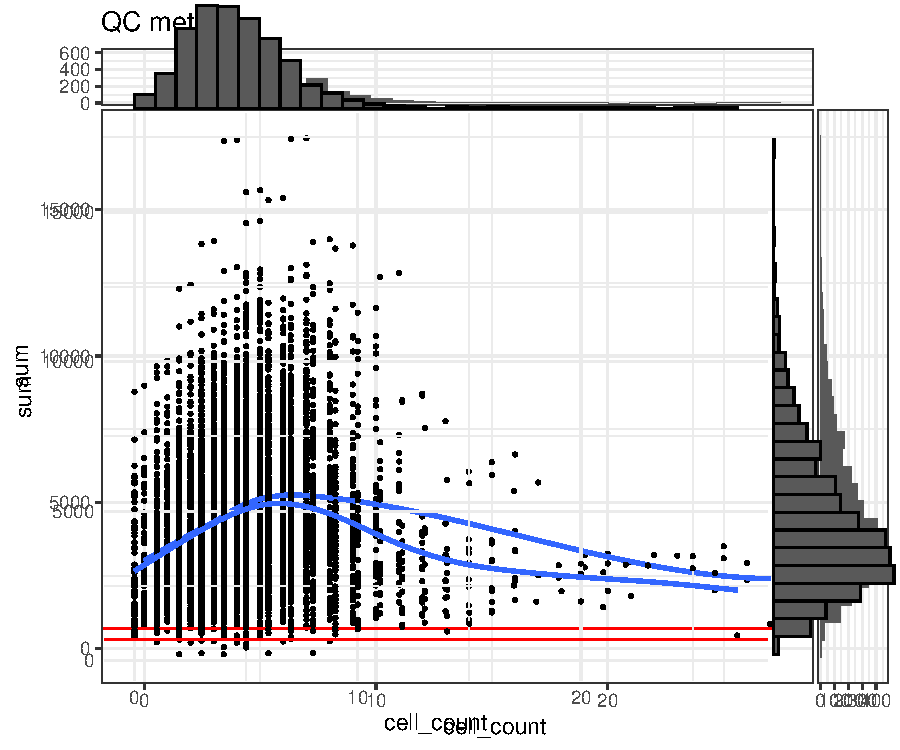
\includegraphics{_main_files/figure-latex/02_plot-libSizeVScelNo-1.pdf}

We need to keep in mind here that the threshold is, to an extent, arbitrary. It is therefore important to look at the number of spots that are left out of the dataset by this choice of cut-off value, and also have a look at their putative spatial patterns. If we filtered out spots with biological relevance, then we should observe some patterns on the tissue map that correlate with some of the known biological structures of the tissue. If we do observe such a phenomenon, we have probably set our threshold too high (i.e.~not permissive enough).

\begin{Shaded}
\begin{Highlighting}[]
\DocumentationTok{\#\# Select library size threshold}
\NormalTok{qc\_lib\_size }\OtherTok{\textless{}{-}} \FunctionTok{colData}\NormalTok{(spe)}\SpecialCharTok{$}\NormalTok{sum }\SpecialCharTok{\textless{}} \DecValTok{700}
\DocumentationTok{\#\# Check how many spots are filtered out}
\FunctionTok{table}\NormalTok{(qc\_lib\_size)}
\end{Highlighting}
\end{Shaded}

\begin{verbatim}
## qc_lib_size
## FALSE  TRUE 
##  3628    11
\end{verbatim}

\begin{Shaded}
\begin{Highlighting}[]
\DocumentationTok{\#\# Add threshold in colData}
\FunctionTok{colData}\NormalTok{(spe)}\SpecialCharTok{$}\NormalTok{qc\_lib\_size }\OtherTok{\textless{}{-}}\NormalTok{ qc\_lib\_size}

\DocumentationTok{\#\# Check putative spatial patterns of removed spots}
\FunctionTok{plotQC}\NormalTok{(spe, }\AttributeTok{type =} \StringTok{"spots"}\NormalTok{, }
       \AttributeTok{discard =} \StringTok{"qc\_lib\_size"}\NormalTok{)}
\end{Highlighting}
\end{Shaded}

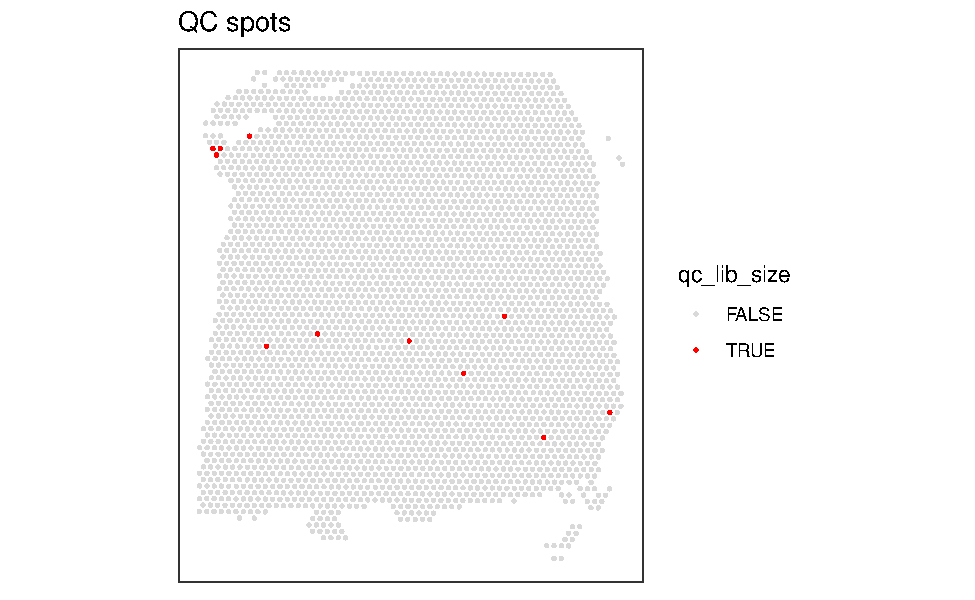
\includegraphics{_main_files/figure-latex/02_libSize-thresh-1.pdf}

As an optional exercise, try to illustrate what happens if we set the threshold too high (i.e., 2000 UMI counts).

\textbf{NOTE:} For reference, remember the ground truth layers in this dataset that we plotted (@ref(fig:02\_plot-maps-gTruth)) at the beginning of this session.

\begin{Shaded}
\begin{Highlighting}[]
\DocumentationTok{\#\# Select library size threshold}
\NormalTok{code...}
\DocumentationTok{\#\# Check how many spots are filtered out}
\NormalTok{code...}
\DocumentationTok{\#\# Add threshold in colData}
\NormalTok{code...}

\DocumentationTok{\#\# Check putative spatial patterns of removed spots}
\FunctionTok{plotQC}\NormalTok{(...)}
\end{Highlighting}
\end{Shaded}

\hypertarget{number-of-expressed-genes}{%
\subsection{Number of expressed genes}\label{number-of-expressed-genes}}

As we did with the library sizes, we can plot a histogram of the number of expressed genes across spots. A gene is ``expressed'' in a spot if it has at least one count in it. We can find this information in the \texttt{detected} column in the \texttt{colData}.

We will follow the same logic for the plots as we did for the library size earlier.

\begin{Shaded}
\begin{Highlighting}[]
\DocumentationTok{\#\# Density and histogram of expressed genes}
\FunctionTok{ggplot}\NormalTok{(}\AttributeTok{data =} \FunctionTok{as.data.frame}\NormalTok{(}\FunctionTok{colData}\NormalTok{(spe)),}
       \FunctionTok{aes}\NormalTok{(}\AttributeTok{x =}\NormalTok{ detected)) }\SpecialCharTok{+}
  \FunctionTok{geom\_histogram}\NormalTok{(}\FunctionTok{aes}\NormalTok{(}\AttributeTok{y =} \FunctionTok{after\_stat}\NormalTok{(density)), }
                 \AttributeTok{colour =} \StringTok{"black"}\NormalTok{, }
                 \AttributeTok{fill =} \StringTok{"grey"}\NormalTok{) }\SpecialCharTok{+}
  \FunctionTok{geom\_density}\NormalTok{(}\AttributeTok{alpha =} \FloatTok{0.5}\NormalTok{,}
               \AttributeTok{adjust =} \FloatTok{1.0}\NormalTok{,}
               \AttributeTok{fill =} \StringTok{"\#A0CBE8"}\NormalTok{,}
               \AttributeTok{colour =} \StringTok{"\#4E79A7"}\NormalTok{) }\SpecialCharTok{+}
  \FunctionTok{scale\_x\_continuous}\NormalTok{(}\AttributeTok{breaks =}\NormalTok{ scales}\SpecialCharTok{::}\FunctionTok{pretty\_breaks}\NormalTok{(}\AttributeTok{n =} \DecValTok{10}\NormalTok{)) }\SpecialCharTok{+} 
  \FunctionTok{scale\_y\_continuous}\NormalTok{(}\AttributeTok{breaks =}\NormalTok{ scales}\SpecialCharTok{::}\FunctionTok{pretty\_breaks}\NormalTok{(}\AttributeTok{n =} \DecValTok{10}\NormalTok{)) }\SpecialCharTok{+} 
  \FunctionTok{xlab}\NormalTok{(}\StringTok{"Genes expressed in each spot"}\NormalTok{) }\SpecialCharTok{+} 
  \FunctionTok{ylab}\NormalTok{(}\StringTok{"Density"}\NormalTok{) }\SpecialCharTok{+} 
  \FunctionTok{theme\_classic}\NormalTok{()}
\end{Highlighting}
\end{Shaded}

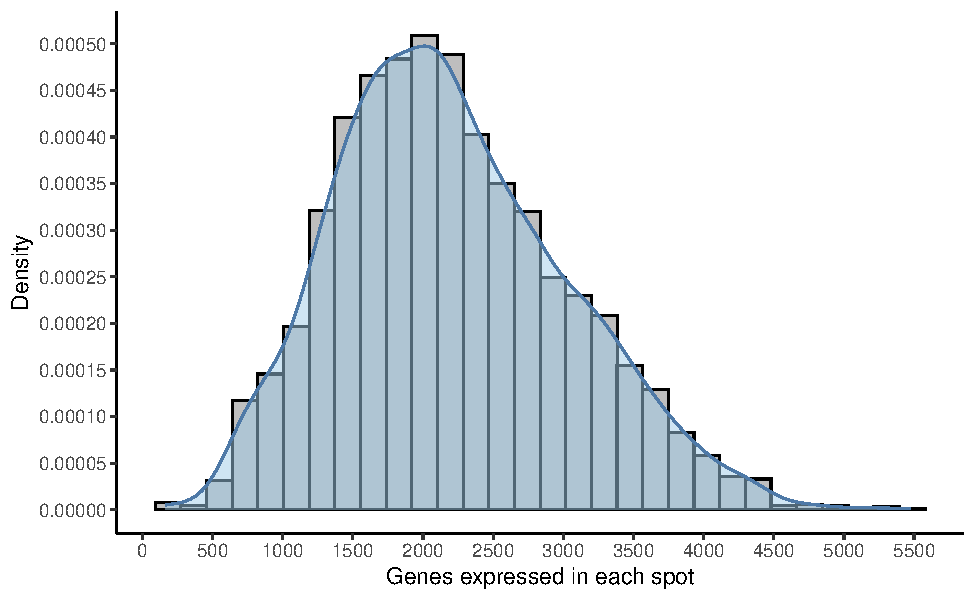
\includegraphics{_main_files/figure-latex/02_plot-genesInSpot-histo-1.pdf}

\begin{Shaded}
\begin{Highlighting}[]
\CommentTok{\# plot number of expressed genes vs. number of cells per spot}
\NormalTok{p }\OtherTok{=} \FunctionTok{ggplot}\NormalTok{(}\FunctionTok{as.data.frame}\NormalTok{(}\FunctionTok{colData}\NormalTok{(spe)), }\FunctionTok{aes}\NormalTok{(}\AttributeTok{x=}\NormalTok{cell\_count, }\AttributeTok{y=}\NormalTok{detected)) }\SpecialCharTok{+}
  \FunctionTok{geom\_point}\NormalTok{(}\AttributeTok{size=}\FloatTok{0.5}\NormalTok{) }\SpecialCharTok{+} 
  \FunctionTok{geom\_smooth}\NormalTok{(}\AttributeTok{se=}\ConstantTok{FALSE}\NormalTok{) }\SpecialCharTok{+}
  \FunctionTok{geom\_hline}\NormalTok{(}\AttributeTok{yintercept =} \DecValTok{500}\NormalTok{, }\AttributeTok{colour=}\StringTok{\textquotesingle{}red\textquotesingle{}}\NormalTok{) }\SpecialCharTok{+} 
  \FunctionTok{theme\_minimal}\NormalTok{()}
\FunctionTok{ggMarginal}\NormalTok{(p, }\AttributeTok{type=}\StringTok{\textquotesingle{}histogram\textquotesingle{}}\NormalTok{, }\AttributeTok{margins =} \StringTok{\textquotesingle{}both\textquotesingle{}}\NormalTok{)}
\end{Highlighting}
\end{Shaded}

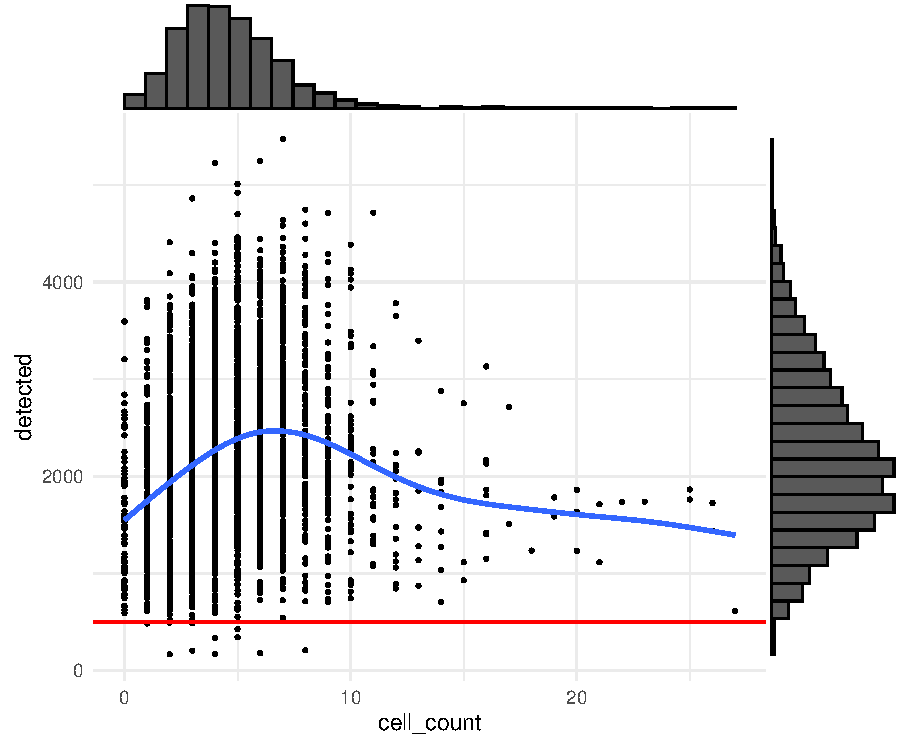
\includegraphics{_main_files/figure-latex/02_genesInSpot-scatter-1.pdf}

Finally, again as before, we apply the chosen threshold to flag spots with (in this case) fewer than 500 expressed genes.

\begin{Shaded}
\begin{Highlighting}[]
\DocumentationTok{\#\# Select expressed genes threshold}
\NormalTok{qc\_detected }\OtherTok{\textless{}{-}} \FunctionTok{colData}\NormalTok{(spe)}\SpecialCharTok{$}\NormalTok{detected }\SpecialCharTok{\textless{}} \DecValTok{500}
\DocumentationTok{\#\# Check how many spots are filtered out}
\FunctionTok{table}\NormalTok{(qc\_detected)}
\end{Highlighting}
\end{Shaded}

\begin{verbatim}
## qc_detected
## FALSE  TRUE 
##  3628    11
\end{verbatim}

\begin{Shaded}
\begin{Highlighting}[]
\DocumentationTok{\#\# Add threshold in colData}
\FunctionTok{colData}\NormalTok{(spe)}\SpecialCharTok{$}\NormalTok{qc\_detected }\OtherTok{\textless{}{-}}\NormalTok{ qc\_detected}

\DocumentationTok{\#\# Check for putative spatial pattern of removed spots}
\FunctionTok{plotQC}\NormalTok{(spe, }\AttributeTok{type =} \StringTok{"spots"}\NormalTok{, }
       \AttributeTok{discard =} \StringTok{"qc\_detected"}\NormalTok{)}
\end{Highlighting}
\end{Shaded}

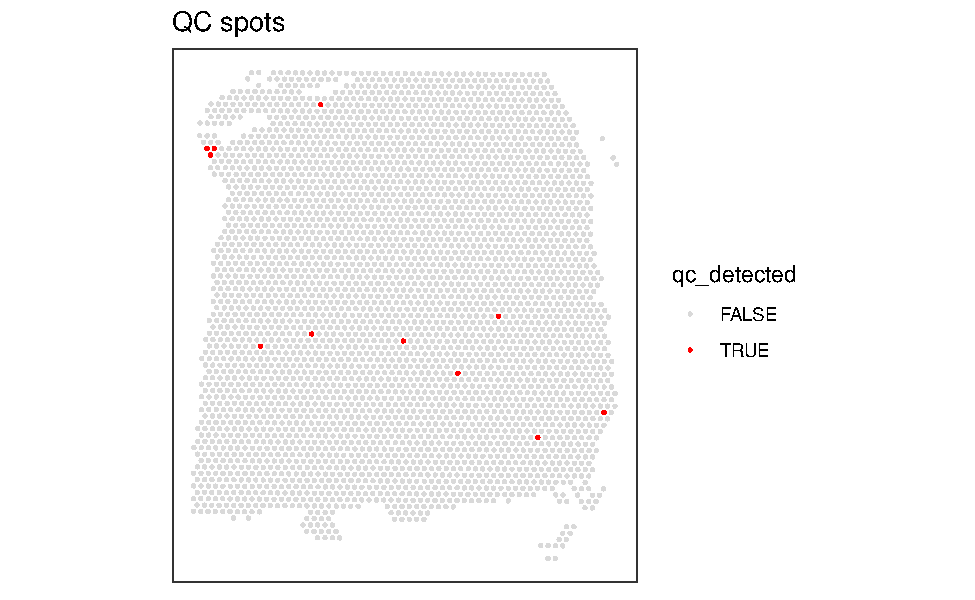
\includegraphics{_main_files/figure-latex/02_genesInSpot-thresh-1.pdf}

Again, an optional exercise is provided to see the effects of an over-enthusiastic filter - to illustrate what happens if we set the threshold too high (i.e., 1000 expressed genes).

\textbf{NOTE:} For reference, remember the ground truth layers in this dataset that we plotted (@ref(fig:02\_plot-maps-gTruth)) at the beginning of this session.

\begin{Shaded}
\begin{Highlighting}[]
\DocumentationTok{\#\# Select library size threshold}
\NormalTok{code...}
\DocumentationTok{\#\# Check how many spots are filtered out}
\NormalTok{code...}
\DocumentationTok{\#\# Add threshold in colData}
\NormalTok{code...}

\DocumentationTok{\#\# Check putative spatial patterns of removed spots}
\FunctionTok{plotQC}\NormalTok{(...)}
\end{Highlighting}
\end{Shaded}

\hypertarget{percentage-of-mitochondrial-expression}{%
\subsection{Percentage of mitochondrial expression}\label{percentage-of-mitochondrial-expression}}

As we briefly touched at the beginning, a high proportion of mitochondrial reads indicates low cell quality, probably due to cell damage.

We calculated this data earlier on in this session, and can now investigate the percentage of mitochondrial expression across spots by looking at the column \texttt{subsets\_mito\_percent} in the \texttt{colData}.

\begin{Shaded}
\begin{Highlighting}[]
\DocumentationTok{\#\# Density and histogram of percentage of mitochondrial expression}
\FunctionTok{ggplot}\NormalTok{(}\AttributeTok{data =} \FunctionTok{as.data.frame}\NormalTok{(}\FunctionTok{colData}\NormalTok{(spe)),}
       \FunctionTok{aes}\NormalTok{(}\AttributeTok{x =}\NormalTok{ subsets\_mito\_percent)) }\SpecialCharTok{+}
  \FunctionTok{geom\_histogram}\NormalTok{(}\FunctionTok{aes}\NormalTok{(}\AttributeTok{y =} \FunctionTok{after\_stat}\NormalTok{(density)), }
                 \AttributeTok{colour =} \StringTok{"black"}\NormalTok{, }
                 \AttributeTok{fill =} \StringTok{"grey"}\NormalTok{) }\SpecialCharTok{+}
  \FunctionTok{geom\_density}\NormalTok{(}\AttributeTok{alpha =} \FloatTok{0.5}\NormalTok{,}
               \AttributeTok{adjust =} \FloatTok{1.0}\NormalTok{,}
               \AttributeTok{fill =} \StringTok{"\#A0CBE8"}\NormalTok{,}
               \AttributeTok{colour =} \StringTok{"\#4E79A7"}\NormalTok{) }\SpecialCharTok{+}
  \FunctionTok{scale\_x\_continuous}\NormalTok{(}\AttributeTok{breaks =}\NormalTok{ scales}\SpecialCharTok{::}\FunctionTok{pretty\_breaks}\NormalTok{(}\AttributeTok{n =} \DecValTok{10}\NormalTok{)) }\SpecialCharTok{+} 
  \FunctionTok{scale\_y\_continuous}\NormalTok{(}\AttributeTok{breaks =}\NormalTok{ scales}\SpecialCharTok{::}\FunctionTok{pretty\_breaks}\NormalTok{(}\AttributeTok{n =} \DecValTok{10}\NormalTok{)) }\SpecialCharTok{+} 
  \FunctionTok{xlab}\NormalTok{(}\StringTok{"Percentage of mitochondrial expression"}\NormalTok{) }\SpecialCharTok{+} 
  \FunctionTok{ylab}\NormalTok{(}\StringTok{"Density"}\NormalTok{) }\SpecialCharTok{+} 
  \FunctionTok{theme\_classic}\NormalTok{()}
\end{Highlighting}
\end{Shaded}

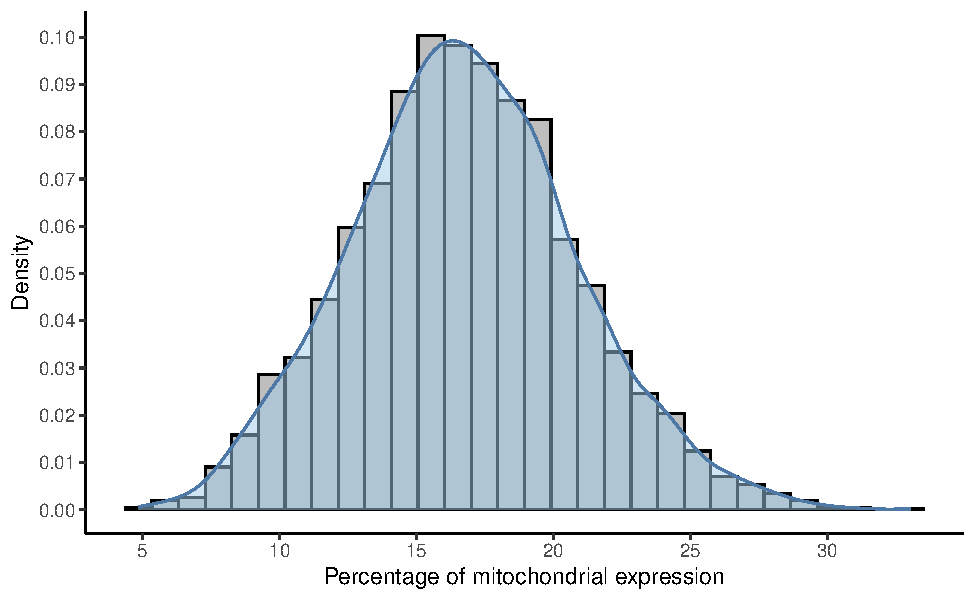
\includegraphics{_main_files/figure-latex/02_plot-mitoPercent-histo-1.pdf}

In this instance, a higher percentage of mitochondrial expression is the thing to avoid, so the threshold is an upper bound, rather than the lower bounds we have observed so far. The suggestion this time is to cut-off at 28\%.

\begin{Shaded}
\begin{Highlighting}[]
\CommentTok{\# plot mitochondrial read proportion vs. number of cells per spot}
\NormalTok{p }\OtherTok{=} \FunctionTok{ggplot}\NormalTok{(}\FunctionTok{as.data.frame}\NormalTok{(}\FunctionTok{colData}\NormalTok{(spe)), }\FunctionTok{aes}\NormalTok{(}\AttributeTok{x=}\NormalTok{cell\_count, }\AttributeTok{y=}\NormalTok{subsets\_mito\_percent)) }\SpecialCharTok{+}
  \FunctionTok{geom\_point}\NormalTok{(}\AttributeTok{size=}\FloatTok{0.5}\NormalTok{) }\SpecialCharTok{+} 
  \FunctionTok{geom\_smooth}\NormalTok{(}\AttributeTok{se=}\ConstantTok{FALSE}\NormalTok{) }\SpecialCharTok{+}
  \FunctionTok{geom\_hline}\NormalTok{(}\AttributeTok{yintercept =} \DecValTok{28}\NormalTok{, }\AttributeTok{colour=}\StringTok{\textquotesingle{}red\textquotesingle{}}\NormalTok{) }\SpecialCharTok{+} 
  \FunctionTok{theme\_minimal}\NormalTok{()}
\FunctionTok{ggMarginal}\NormalTok{(p, }\AttributeTok{type=}\StringTok{\textquotesingle{}histogram\textquotesingle{}}\NormalTok{)}
\end{Highlighting}
\end{Shaded}

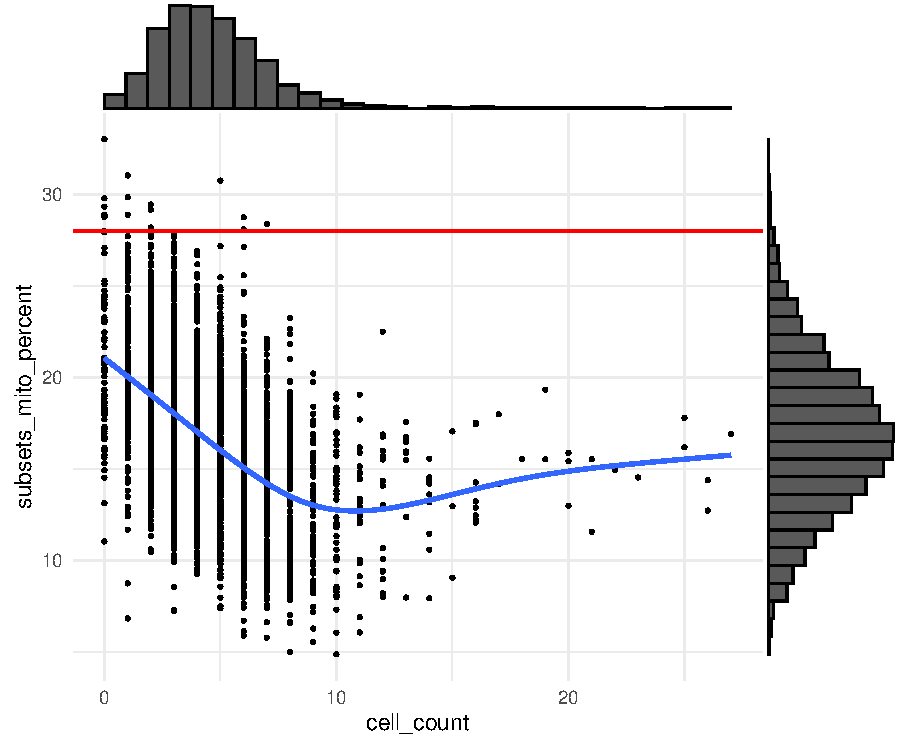
\includegraphics{_main_files/figure-latex/02_mitoPercent-scatter-1.pdf}

\begin{Shaded}
\begin{Highlighting}[]
\DocumentationTok{\#\# Select expressed genes threshold}
\NormalTok{qc\_mito }\OtherTok{\textless{}{-}} \FunctionTok{colData}\NormalTok{(spe)}\SpecialCharTok{$}\NormalTok{subsets\_mito\_percent }\SpecialCharTok{\textgreater{}} \DecValTok{28}
\DocumentationTok{\#\# Check how many spots are filtered out}
\FunctionTok{table}\NormalTok{(qc\_mito)}
\end{Highlighting}
\end{Shaded}

\begin{verbatim}
## qc_mito
## FALSE  TRUE 
##  3622    17
\end{verbatim}

\begin{Shaded}
\begin{Highlighting}[]
\DocumentationTok{\#\# Add threshold in colData}
\FunctionTok{colData}\NormalTok{(spe)}\SpecialCharTok{$}\NormalTok{qc\_mito }\OtherTok{\textless{}{-}}\NormalTok{ qc\_mito}

\DocumentationTok{\#\# Check for putative spatial pattern of removed spots}
\FunctionTok{plotQC}\NormalTok{(spe, }\AttributeTok{type =} \StringTok{"spots"}\NormalTok{, }
       \AttributeTok{discard =} \StringTok{"qc\_mito"}\NormalTok{)}
\end{Highlighting}
\end{Shaded}

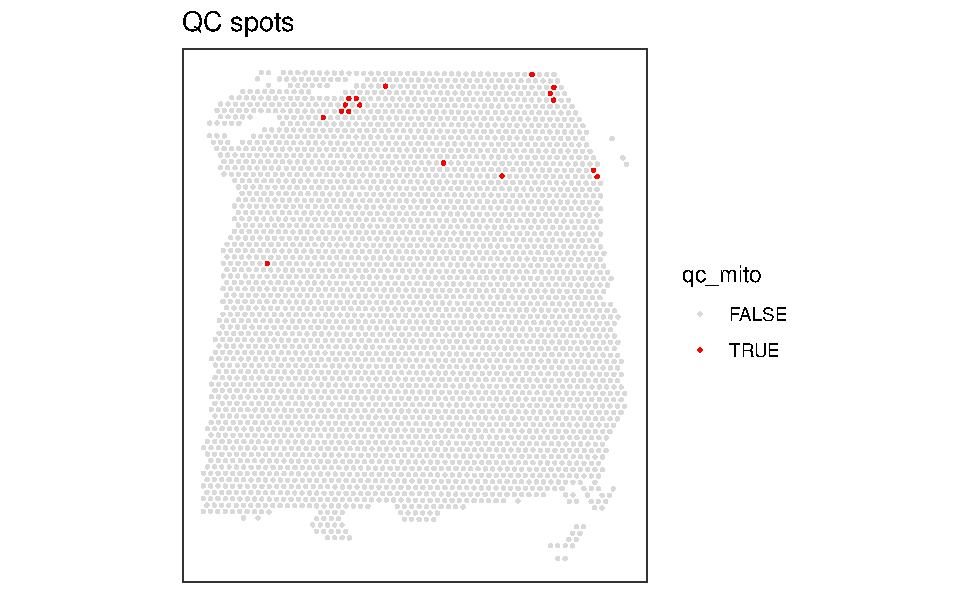
\includegraphics{_main_files/figure-latex/02_mitoPercent-thresh-1.pdf}

Again, try to illustrate what happens if we set the threshold too low (i.e., 20 0r 25\%).

\textbf{NOTE:} For reference, remember the ground truth layers in this dataset that we plotted (@ref(fig:02\_plot-maps-gTruth)) at the beginning of this session.

\begin{Shaded}
\begin{Highlighting}[]
\DocumentationTok{\#\# Select library size threshold}
\NormalTok{code...}
\DocumentationTok{\#\# Check how many spots are filtered out}
\NormalTok{code...}
\DocumentationTok{\#\# Add threshold in colData}
\NormalTok{code...}

\DocumentationTok{\#\# Check putative spatial patterns of removed spots}
\FunctionTok{plotQC}\NormalTok{(...)}
\end{Highlighting}
\end{Shaded}

\hypertarget{number-of-cells-per-spot}{%
\subsection{Number of cells per spot}\label{number-of-cells-per-spot}}

Number of cells per spot is an attribute that not all datasets include. Nonetheless, it can be useful to further control the quality of the dataset prior to any downstream analysis. Of course, the number of cells per spot depends on the tissue type and organism and according to \href{https://kb.10xgenomics.com/hc/en-us/articles/360035487952-How-many-cells-are-captured-in-a-single-spot-}{10X Genomics}, each spot typically contains between 0 and 10 cells.

The DPFLC dataset does contain information on the number of cells per spot (acquired by processing and cell segmentation of high-resolution histology images obtained prior on-slide cDNA synthesis, see \citet{Maynard2021Mar} for details). To investigate the number of cells in each spot looking for any outlier values that could indicate problems we need to take a look in the column \texttt{cell\_count} in the \texttt{colData}.

\begin{Shaded}
\begin{Highlighting}[]
\DocumentationTok{\#\# Density and histogram of the number of cells in each spot}
\FunctionTok{ggplot}\NormalTok{(}\AttributeTok{data =} \FunctionTok{as.data.frame}\NormalTok{(}\FunctionTok{colData}\NormalTok{(spe)),}
       \FunctionTok{aes}\NormalTok{(}\AttributeTok{x =}\NormalTok{ cell\_count)) }\SpecialCharTok{+}
  \FunctionTok{geom\_histogram}\NormalTok{(}\FunctionTok{aes}\NormalTok{(}\AttributeTok{y =} \FunctionTok{after\_stat}\NormalTok{(density)), }
                 \AttributeTok{binwidth =} \DecValTok{1}\NormalTok{,}
                 \AttributeTok{colour =} \StringTok{"black"}\NormalTok{, }
                 \AttributeTok{fill =} \StringTok{"grey"}\NormalTok{) }\SpecialCharTok{+}
  \FunctionTok{geom\_density}\NormalTok{(}\AttributeTok{alpha =} \FloatTok{0.5}\NormalTok{,}
               \AttributeTok{adjust =} \FloatTok{1.5}\NormalTok{,}
               \AttributeTok{fill =} \StringTok{"\#A0CBE8"}\NormalTok{,}
               \AttributeTok{colour =} \StringTok{"\#4E79A7"}\NormalTok{) }\SpecialCharTok{+}
  \FunctionTok{scale\_x\_continuous}\NormalTok{(}\AttributeTok{breaks =}\NormalTok{ scales}\SpecialCharTok{::}\FunctionTok{pretty\_breaks}\NormalTok{(}\AttributeTok{n =} \DecValTok{10}\NormalTok{)) }\SpecialCharTok{+} 
  \FunctionTok{scale\_y\_continuous}\NormalTok{(}\AttributeTok{breaks =}\NormalTok{ scales}\SpecialCharTok{::}\FunctionTok{pretty\_breaks}\NormalTok{(}\AttributeTok{n =} \DecValTok{10}\NormalTok{)) }\SpecialCharTok{+} 
  \FunctionTok{xlab}\NormalTok{(}\StringTok{"Number of cells per spot"}\NormalTok{) }\SpecialCharTok{+} 
  \FunctionTok{ylab}\NormalTok{(}\StringTok{"Density"}\NormalTok{) }\SpecialCharTok{+} 
  \FunctionTok{theme\_classic}\NormalTok{()}
\end{Highlighting}
\end{Shaded}

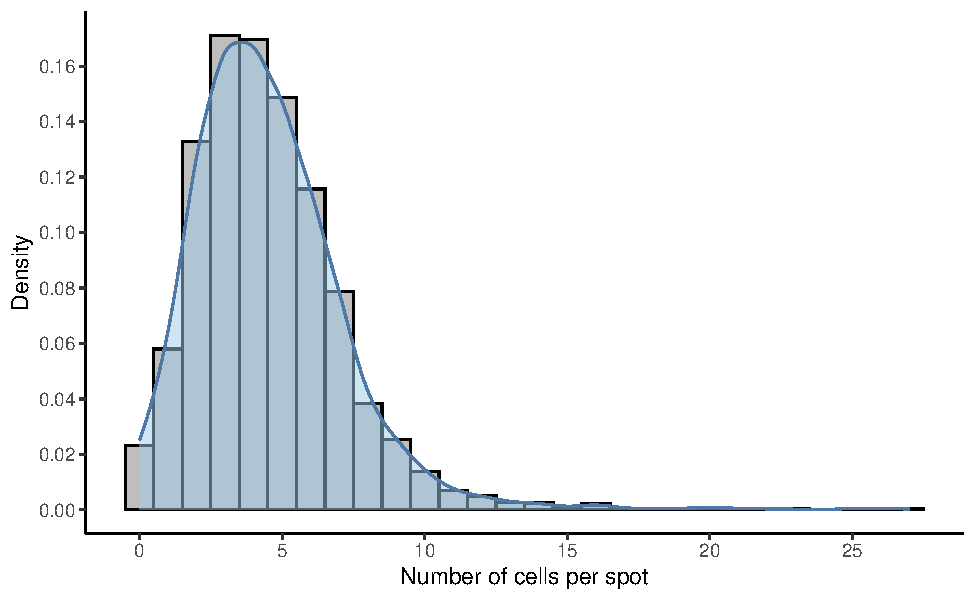
\includegraphics{_main_files/figure-latex/02_plot-cellsPerSpot-histo-1.pdf}

\begin{Shaded}
\begin{Highlighting}[]
\DocumentationTok{\#\# Have a look at the values}
\FunctionTok{table}\NormalTok{(}\FunctionTok{colData}\NormalTok{(spe)}\SpecialCharTok{$}\NormalTok{cell\_count)}
\end{Highlighting}
\end{Shaded}

\begin{verbatim}
## 
##   0   1   2   3   4   5   6   7   8   9  10  11  12  13  14  15  16  17  18  19 
##  84 211 483 623 617 541 421 287 140  92  50  25  18  10   9   3   8   2   1   2 
##  20  21  22  23  25  26  27 
##   3   2   1   1   2   2   1
\end{verbatim}

\begin{Shaded}
\begin{Highlighting}[]
\CommentTok{\# plot number of expressed genes vs. number of cells per spot}
\NormalTok{p }\OtherTok{=} \FunctionTok{ggplot}\NormalTok{(}\FunctionTok{as.data.frame}\NormalTok{(}\FunctionTok{colData}\NormalTok{(spe)), }\FunctionTok{aes}\NormalTok{(}\AttributeTok{x=}\NormalTok{cell\_count, }\AttributeTok{y=}\NormalTok{detected)) }\SpecialCharTok{+}
  \FunctionTok{geom\_point}\NormalTok{() }\SpecialCharTok{+} 
  \FunctionTok{geom\_smooth}\NormalTok{(}\AttributeTok{se=}\ConstantTok{FALSE}\NormalTok{) }\SpecialCharTok{+}
  \FunctionTok{geom\_vline}\NormalTok{(}\AttributeTok{xintercept =} \DecValTok{10}\NormalTok{, }\AttributeTok{colour=}\StringTok{\textquotesingle{}red\textquotesingle{}}\NormalTok{) }\SpecialCharTok{+} 
  \FunctionTok{theme\_minimal}\NormalTok{()}
\FunctionTok{ggMarginal}\NormalTok{(p, }\AttributeTok{type=}\StringTok{\textquotesingle{}histogram\textquotesingle{}}\NormalTok{)}
\end{Highlighting}
\end{Shaded}

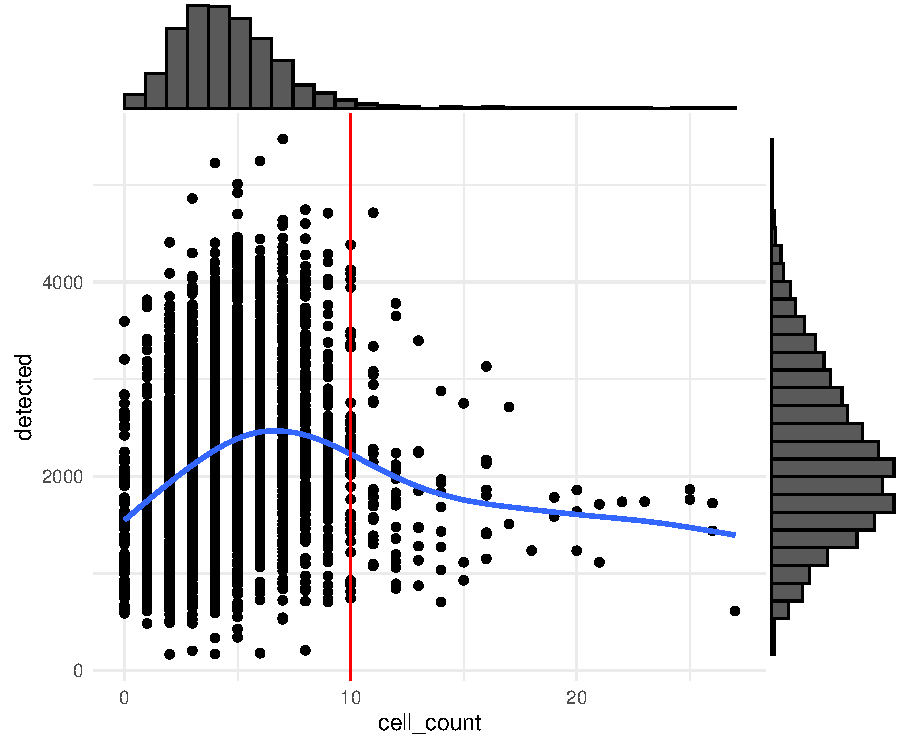
\includegraphics{_main_files/figure-latex/02_cellsPerSpot-scatter-1.pdf}

As we can see from both the histogram and the scatter plot there is a tail of very high values, which could indicate problems for these spots. More specifically, we can see from the scatter plot that most of the spots with very high cell counts also tend to have lower numbers of expressed genes. This indicates problems with the experiment on these spots, and they should be removed.

\begin{Shaded}
\begin{Highlighting}[]
\DocumentationTok{\#\# Select expressed genes threshold}
\NormalTok{qc\_cell\_count }\OtherTok{\textless{}{-}} \FunctionTok{colData}\NormalTok{(spe)}\SpecialCharTok{$}\NormalTok{cell\_count }\SpecialCharTok{\textgreater{}} \DecValTok{10}
\DocumentationTok{\#\# Check how many spots are filtered out}
\FunctionTok{table}\NormalTok{(qc\_cell\_count)}
\end{Highlighting}
\end{Shaded}

\begin{verbatim}
## qc_cell_count
## FALSE  TRUE 
##  3549    90
\end{verbatim}

\begin{Shaded}
\begin{Highlighting}[]
\DocumentationTok{\#\# Add threshold in colData}
\FunctionTok{colData}\NormalTok{(spe)}\SpecialCharTok{$}\NormalTok{qc\_cell\_count }\OtherTok{\textless{}{-}}\NormalTok{ qc\_cell\_count}

\DocumentationTok{\#\# Check for putative spatial pattern of removed spots}
\FunctionTok{plotQC}\NormalTok{(spe, }\AttributeTok{type =} \StringTok{"spots"}\NormalTok{, }
       \AttributeTok{discard =} \StringTok{"qc\_cell\_count"}\NormalTok{)}
\end{Highlighting}
\end{Shaded}

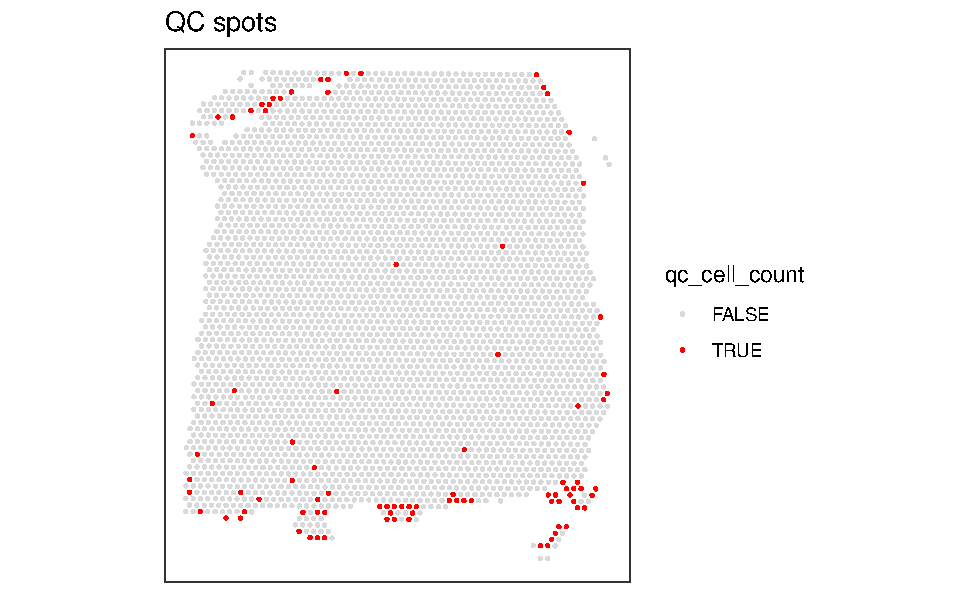
\includegraphics{_main_files/figure-latex/02_cellsPerSpot-thresh-1.pdf}

While there is a spatial pattern to the discarded spots, it does not appear to be correlated with the known biological features (cortical layers). The discarded spots are typically at the edges of the tissue. It seems plausible that something has gone wrong with the cell segmentation on the edges of the images, so it makes sense to remove these spots.

\hypertarget{remove-low-quality-spots}{%
\subsection{Remove low-quality spots}\label{remove-low-quality-spots}}

All the steps so far have flagged spots with potential issues - before proceeding with analysis, we want to remove these spots from our SpatialExperiment object. Since we have calculated different spot-level QC metrics and selected thresholds for each one, we can combine them to identify a set of low-quality spots, and remove them from our \texttt{spe} object in a single step.

We can also check once more that the combined set of discarded spots does not correspond to any obvious biologically relevant group of spots.

\begin{Shaded}
\begin{Highlighting}[]
\DocumentationTok{\#\# Check the number of discarded spots for each metric}
\FunctionTok{apply}\NormalTok{(}\FunctionTok{cbind}\NormalTok{(qc\_lib\_size, qc\_detected, qc\_mito, qc\_cell\_count), }\DecValTok{2}\NormalTok{, sum)}
\end{Highlighting}
\end{Shaded}

\begin{verbatim}
##   qc_lib_size   qc_detected       qc_mito qc_cell_count 
##            11            11            17            90
\end{verbatim}

\begin{Shaded}
\begin{Highlighting}[]
\DocumentationTok{\#\# Combine together the set of discarded spots}
\NormalTok{discard }\OtherTok{\textless{}{-}}\NormalTok{ qc\_lib\_size }\SpecialCharTok{|}\NormalTok{ qc\_detected }\SpecialCharTok{|}\NormalTok{ qc\_mito }\SpecialCharTok{|}\NormalTok{ qc\_cell\_count}
\DocumentationTok{\#\# Store the set in the object}
\FunctionTok{colData}\NormalTok{(spe)}\SpecialCharTok{$}\NormalTok{discard }\OtherTok{\textless{}{-}}\NormalTok{ discard}

\DocumentationTok{\#\# Check the spatial pattern of combined set of discarded spots}
\FunctionTok{plotQC}\NormalTok{(spe, }\AttributeTok{type =} \StringTok{"spots"}\NormalTok{, }
       \AttributeTok{discard =} \StringTok{"discard"}\NormalTok{)}
\end{Highlighting}
\end{Shaded}

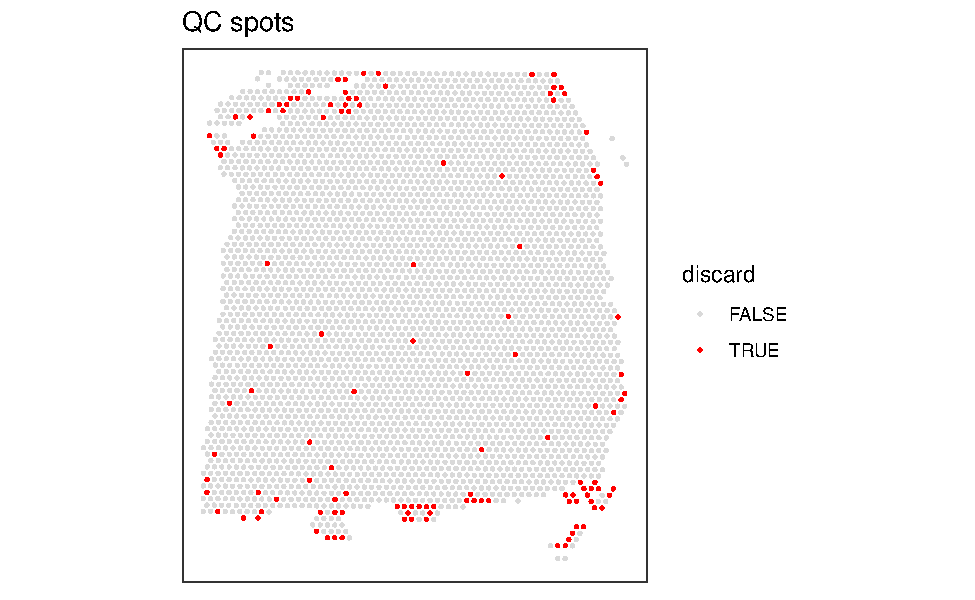
\includegraphics{_main_files/figure-latex/02_checkQC-thresh-1.pdf}

Since this dataset has also manual annotation (remember @ref(fig:02\_plot-maps-gTruth)) we see that there are locations that are not annotated (marked with \texttt{NA}). We could further remove those locations to reduce potential noise and further increase the quality of the dataset.

\begin{Shaded}
\begin{Highlighting}[]
\DocumentationTok{\#\# Select locations without annotation}
\NormalTok{qc\_NA\_spots }\OtherTok{\textless{}{-}} \FunctionTok{is.na}\NormalTok{(}\FunctionTok{colData}\NormalTok{(spe)}\SpecialCharTok{$}\NormalTok{ground\_truth)}
\DocumentationTok{\#\# Combine together the set of discarded spots}
\NormalTok{discard }\OtherTok{\textless{}{-}}\NormalTok{ qc\_lib\_size }\SpecialCharTok{|}\NormalTok{ qc\_detected }\SpecialCharTok{|}\NormalTok{ qc\_mito }\SpecialCharTok{|}\NormalTok{ qc\_cell\_count }\SpecialCharTok{|}\NormalTok{ qc\_NA\_spots}
\DocumentationTok{\#\# Store the set in the object}
\FunctionTok{colData}\NormalTok{(spe)}\SpecialCharTok{$}\NormalTok{discard }\OtherTok{\textless{}{-}}\NormalTok{ discard}

\DocumentationTok{\#\# Check the spatial pattern of combined set of discarded spots}
\FunctionTok{plotQC}\NormalTok{(spe, }\AttributeTok{type =} \StringTok{"spots"}\NormalTok{, }
       \AttributeTok{discard =} \StringTok{"discard"}\NormalTok{)}
\end{Highlighting}
\end{Shaded}

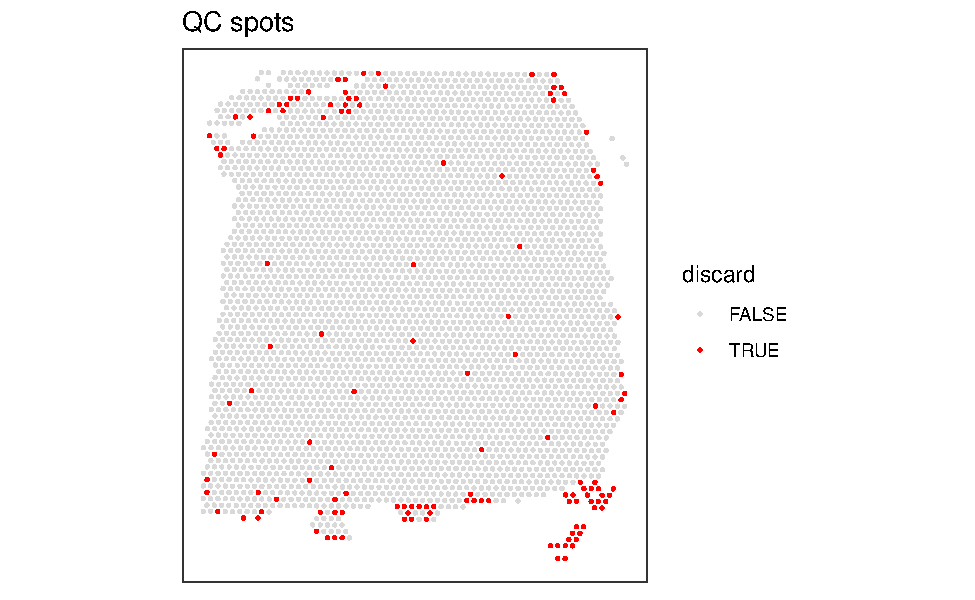
\includegraphics{_main_files/figure-latex/02_notAnnotSpots-1.pdf}

\begin{Shaded}
\begin{Highlighting}[]
\DocumentationTok{\#\# remove combined set of low{-}quality spots}
\NormalTok{spe }\OtherTok{\textless{}{-}}\NormalTok{ spe[, }\SpecialCharTok{!}\FunctionTok{colData}\NormalTok{(spe)}\SpecialCharTok{$}\NormalTok{discard]}
\end{Highlighting}
\end{Shaded}

\hypertarget{normalisation-of-counts}{%
\section{Normalisation of counts}\label{normalisation-of-counts}}

\hypertarget{background}{%
\subsection{Background}\label{background}}

Normalisation is applied in STx data for the same reason as any other RNA-Seq technique - the differences observed in the count data can arise from a range of systematic factors, not just a physiologically-relevant change in expression. The primary systematic effect is that of library size (or in the case of STx, counts/UMIs per spot). \texttt{scater} corrects for library size by scaling the sizes across all spots such that the mean library size is 1. Normalized counts are then calculated as a ratio of observed count to library size factor.

Secondly, a log-transformation is applied to the scaled counts - this transformation is commonly applied as it stabilises the variance across the range of transcriptomics data (otherwise the variance is dominated by highly expressed genes) and it facilitates comparisons of expression by rendering positive and negative changes symmetrical and found by subtraction rather than division. Since \(log2(0)\) is undefined, a \emph{pseudocount} is added to each observed count to avoid this error - a pseudocount of 1 is typically applied, as \(log2(0+1) = 0\).

Here we will be using methods from the \texttt{scater} \citep{McCarthy2017Apr} and \texttt{scran} \citep{Lun2016Oct} packages that calculate logcounts using library size factors. The library size factors approach is arguably the simplest approach for STx data. Other approaches used in scRNA-seq are more difficult to justify their use in STx because of two main reasons:

\begin{enumerate}
\def\labelenumi{\arabic{enumi}.}
\tightlist
\item
  Spots can contain multiple cells of different cell-types.
\item
  Datasets can include multiple tissue samples which will lead to different clusterings.
\end{enumerate}

\hypertarget{log-tranformation-of-counts}{%
\subsection{Log-tranformation of counts}\label{log-tranformation-of-counts}}

\begin{Shaded}
\begin{Highlighting}[]
\DocumentationTok{\#\# Calculate library size factors}
\NormalTok{spe }\OtherTok{\textless{}{-}} \FunctionTok{computeLibraryFactors}\NormalTok{(spe)}
\DocumentationTok{\#\# Have a look at the size factors}
\FunctionTok{summary}\NormalTok{(}\FunctionTok{sizeFactors}\NormalTok{(spe))}
\end{Highlighting}
\end{Shaded}

\begin{verbatim}
##    Min. 1st Qu.  Median    Mean 3rd Qu.    Max. 
##  0.1514  0.6326  0.9011  1.0000  1.2849  3.7500
\end{verbatim}

As described above, the mean size factor is 1.0.

\begin{Shaded}
\begin{Highlighting}[]
\DocumentationTok{\#\# Density and histogram of library sizes}
\FunctionTok{ggplot}\NormalTok{(}\AttributeTok{data =} \FunctionTok{data.frame}\NormalTok{(}\AttributeTok{sFact =} \FunctionTok{sizeFactors}\NormalTok{(spe)), }
       \FunctionTok{aes}\NormalTok{(}\AttributeTok{x =}\NormalTok{ sFact)) }\SpecialCharTok{+}
  \FunctionTok{geom\_histogram}\NormalTok{(}\FunctionTok{aes}\NormalTok{(}\AttributeTok{y =} \FunctionTok{after\_stat}\NormalTok{(density)), }
                 \AttributeTok{colour =} \StringTok{"black"}\NormalTok{, }
                 \AttributeTok{fill =} \StringTok{"grey"}\NormalTok{) }\SpecialCharTok{+}
  \FunctionTok{geom\_density}\NormalTok{(}\AttributeTok{alpha =} \FloatTok{0.5}\NormalTok{,}
               \AttributeTok{adjust =} \FloatTok{1.0}\NormalTok{,}
               \AttributeTok{fill =} \StringTok{"\#A0CBE8"}\NormalTok{,}
               \AttributeTok{colour =} \StringTok{"\#4E79A7"}\NormalTok{) }\SpecialCharTok{+}
  \FunctionTok{scale\_x\_continuous}\NormalTok{(}\AttributeTok{breaks =}\NormalTok{ scales}\SpecialCharTok{::}\FunctionTok{pretty\_breaks}\NormalTok{(}\AttributeTok{n =} \DecValTok{10}\NormalTok{)) }\SpecialCharTok{+} 
  \FunctionTok{scale\_y\_continuous}\NormalTok{(}\AttributeTok{breaks =}\NormalTok{ scales}\SpecialCharTok{::}\FunctionTok{pretty\_breaks}\NormalTok{(}\AttributeTok{n =} \DecValTok{10}\NormalTok{)) }\SpecialCharTok{+} 
  \FunctionTok{xlab}\NormalTok{(}\StringTok{"Library size"}\NormalTok{) }\SpecialCharTok{+} 
  \FunctionTok{ylab}\NormalTok{(}\StringTok{"Density"}\NormalTok{) }\SpecialCharTok{+} 
  \FunctionTok{theme\_classic}\NormalTok{()}
\end{Highlighting}
\end{Shaded}

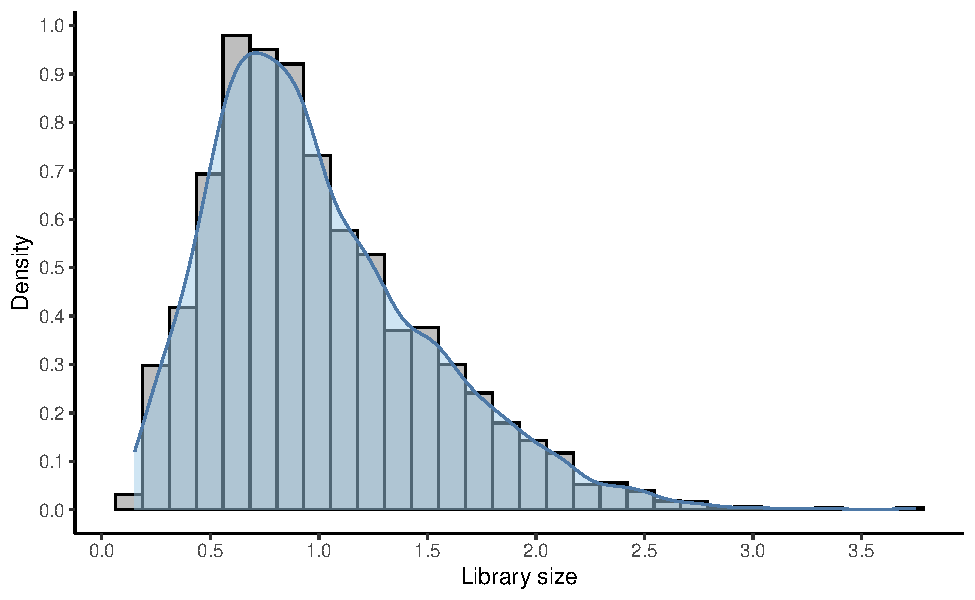
\includegraphics{_main_files/figure-latex/02_plot-labfact-histo-1.pdf}

The log-transformation that takes place is a log2-transformation and in order to avoid \emph{- Infinity} values we add a pseudo value of 1. Both the log2- transformation and the pseudocount of 1 are defaults in this method.

\begin{Shaded}
\begin{Highlighting}[]
\DocumentationTok{\#\# Calculate logcounts and store in the spe object}
\NormalTok{spe }\OtherTok{\textless{}{-}} \FunctionTok{logNormCounts}\NormalTok{(spe)}

\DocumentationTok{\#\# Check that a new assay has been added}
\FunctionTok{assayNames}\NormalTok{(spe)}
\end{Highlighting}
\end{Shaded}

\begin{verbatim}
## [1] "counts"    "logcounts"
\end{verbatim}

\hypertarget{selecting-genes}{%
\section{Selecting genes}\label{selecting-genes}}

\hypertarget{background-1}{%
\subsection{Background}\label{background-1}}

Gene selection - or alternatively ``feature selection'' - is applied to identify genes that are going to be informative for the downstream analyses. The most common feature selection method is the definition of highly variable genes (HVGs). The assumption is that since we quality-controlled and normalised our dataset, the genes with high variability are the ones that contain high levels of biological variability too. Since here we have a spatial dataset we can also try to identify spatially variable genes too (SVGs).

It is important to note that HVGs are identified solely from the gene expression data. Spatial information does not play a role in finding HVGs. STx data pose a dilemma; does the meaningful spatial information reflect only spatial distribution of major cell types or does it reflect additional important spatial features? If we believe the former, relying on HVGs can be enough. If the second also holds true though, it is important to identify SVGs as well.

\hypertarget{highly-variable-genes-hvgs}{%
\subsection{Highly Variable Genes (HVGs)}\label{highly-variable-genes-hvgs}}

Here we will be using methods from the \texttt{scran} package \citep{Lun2016Oct} to identify a set of HVGs. Again, here we need to remember that \texttt{scran} methods were developed for scRNA-seq and we are performing the analysis under the assumption that the spots of an STx experiment can be treated as single cells.

In this dataset, the mitochondrial genes are too highly expressed and are not of major biological interest. As a result, if we are to identify true HVGs, we first need to remove the mitochondrial genes.

\begin{Shaded}
\begin{Highlighting}[]
\DocumentationTok{\#\# Remove mitochondrial genes}
\NormalTok{spe }\OtherTok{\textless{}{-}}\NormalTok{ spe[}\SpecialCharTok{!}\NormalTok{is\_mito, ]}
\end{Highlighting}
\end{Shaded}

Then, we apply methods from \texttt{scran} that give a list of HVGs, which can be used for further downstream analyses.

First we model the variance of the log-expression profiles for each gene, decomposing it into technical and biological components based on a fitted mean-variance trend.

\begin{Shaded}
\begin{Highlighting}[]
\DocumentationTok{\#\# Fit mean{-}variance relationship}
\NormalTok{dec }\OtherTok{\textless{}{-}} \FunctionTok{modelGeneVar}\NormalTok{(spe)}
\DocumentationTok{\#\# Visualize mean{-}variance relationship}
\NormalTok{fit }\OtherTok{\textless{}{-}} \FunctionTok{metadata}\NormalTok{(dec)}
\NormalTok{fit\_df }\OtherTok{\textless{}{-}} \FunctionTok{data.frame}\NormalTok{(}\AttributeTok{mean =}\NormalTok{ fit}\SpecialCharTok{$}\NormalTok{mean,}
                     \AttributeTok{var =}\NormalTok{ fit}\SpecialCharTok{$}\NormalTok{var,}
                     \AttributeTok{trend =}\NormalTok{ fit}\SpecialCharTok{$}\FunctionTok{trend}\NormalTok{(fit}\SpecialCharTok{$}\NormalTok{mean))}

\FunctionTok{ggplot}\NormalTok{(}\AttributeTok{data =}\NormalTok{ fit\_df, }
       \FunctionTok{aes}\NormalTok{(}\AttributeTok{x =}\NormalTok{ mean, }\AttributeTok{y =}\NormalTok{ var)) }\SpecialCharTok{+} 
  \FunctionTok{geom\_point}\NormalTok{() }\SpecialCharTok{+} 
  \FunctionTok{geom\_line}\NormalTok{(}\FunctionTok{aes}\NormalTok{(}\AttributeTok{y =}\NormalTok{ trend), }\AttributeTok{colour =} \StringTok{"dodgerblue"}\NormalTok{, }\AttributeTok{linewidth =} \FloatTok{1.5}\NormalTok{) }\SpecialCharTok{+} 
  \FunctionTok{labs}\NormalTok{(}\AttributeTok{x =} \StringTok{"mean of log{-}expression"}\NormalTok{,}
       \AttributeTok{y =} \StringTok{"variance of log{-}expression"}\NormalTok{) }\SpecialCharTok{+} 
  \FunctionTok{theme\_classic}\NormalTok{()}
\end{Highlighting}
\end{Shaded}

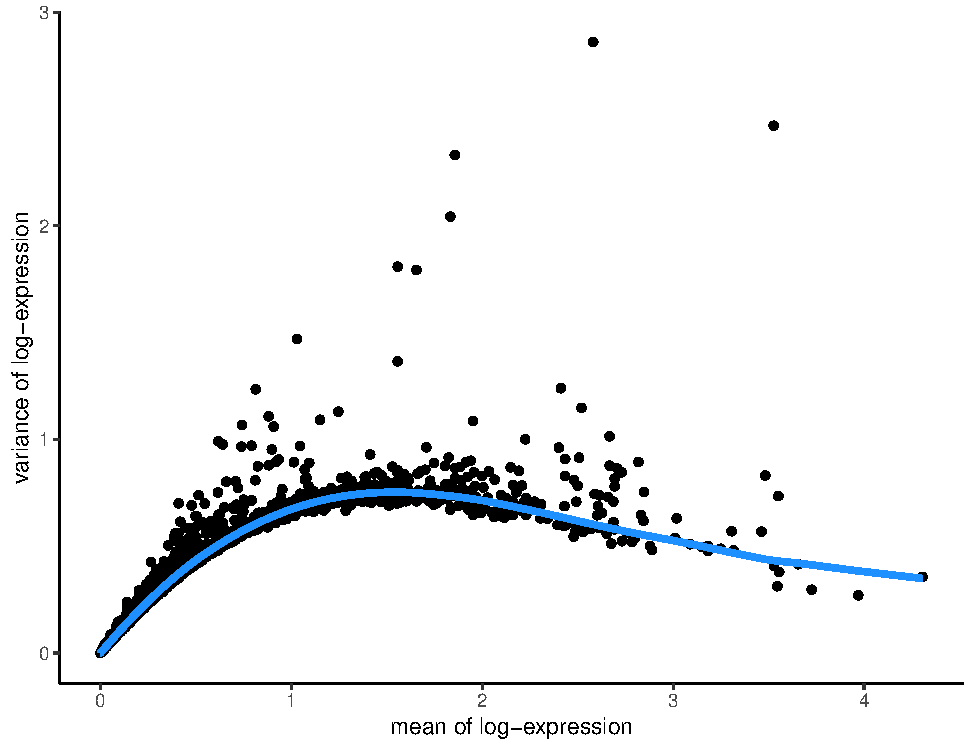
\includegraphics{_main_files/figure-latex/02_features_FitModel-1.pdf}

The \texttt{trend} function that we used above is returned from the \texttt{modelGeneVar} function and returns the fitted value of the trend at any value of the mean. The ``biological'' variance of a gene is what remains when the fitted variance for a gene of that expression value is subtracted from the total variance (so genes above the blue trend line above have a positive biological variance).

We select the top 10\% of genes based on their biological variability The parameter \texttt{prop} defines how many HVGs we want. For example \texttt{prop\ =\ 0.1} returns the top 10\% of genes. \texttt{prop\ =\ 1.0} would return all genes with a positive biological variability.

\begin{Shaded}
\begin{Highlighting}[]
\DocumentationTok{\#\# Select top HVGs}
\NormalTok{top\_hvgs }\OtherTok{\textless{}{-}} \FunctionTok{getTopHVGs}\NormalTok{(dec, }\AttributeTok{prop =} \FloatTok{0.1}\NormalTok{)}

\DocumentationTok{\#\# How many are the HVGs?}
\FunctionTok{length}\NormalTok{(top\_hvgs)}
\end{Highlighting}
\end{Shaded}

\begin{verbatim}
## [1] 1429
\end{verbatim}

\textbf{NOTE} - we will return to feature selection in the next practical, as it is a complicated process with significant impacts on the chosen downstream analysis.

\hypertarget{spatially-variable-genes-svgs}{%
\subsection{Spatially variable genes (SVGs)}\label{spatially-variable-genes-svgs}}

SVGs are genes with a highly spatially correlated pattern of expression, which varies along with the spatial distribution of a tissue structure of interest. This phenomenon is also called \emph{spatial autocorrelation} and underlies all types of spatial data, as we will discuss later.

The field of geography has developed some statistical measures to calculate spatial autocorrelation. Examples of these are Moran's \emph{I} \citep{Moran1950Jun} and Geary's \emph{C} \citep{Geary1954Nov} that can be used to rank genes by the observed spatial autocorrelation to identify SVGs.

Several sophisticated new statistical methods to identify SVGs in STx data have also recently been developed. These include \href{https://github.com/Teichlab/SpatialDE}{SpatialDE} \citep{Svensson2018May}, \href{https://xzhoulab.github.io/SPARK/}{SPARK} \citep{Sun2020Feb}, and \href{https://xzhoulab.github.io/SPARK/}{SPARK-X} \citep{Zhu2021Dec}.

\hypertarget{integration-of-hvgs-and-svgs}{%
\subsection{Integration of HVGs and SVGs}\label{integration-of-hvgs-and-svgs}}

A recent benchmark paper \citep{Li2022Jan} showed that integrating HVGs and SVGs to generate a combined set of features can improve downstream clustering performance in STx data. This confirms that SVGs contain additional biologically relevant information that is not captured by HVGs in these datasets. For example, a simple way to combine these features is to concatenate columns of principal components (PCs) calculated on the set of HVGs and the set of SVGs (excluding overlapping HVGs), and then using the combined set of features for further downstream analyses \citep{Li2022Jan}.

\hypertarget{dimensionality-reduction}{%
\section{Dimensionality reduction}\label{dimensionality-reduction}}

\hypertarget{background-2}{%
\subsection{Background}\label{background-2}}

Dimensionality reduction is an important step prior to any downstream clustering attempts. There are two main ways of reducing the dimensions of a dataset. The gold standard is Principal Components Analysis (PCA) and the other -a more recent one- Uniform manifold Approximation and Projection (UMAP) \citep{McInnes2018Feb}. The main difference between the two is that the distances between the data points in PCA space are interpretable and can be used to cluster the data points while the distances in a UMAP embedding are not interpretable and thus, cannot be used to cluster the data points. As a result, we will be using PCA to reduce the dimensions of our dataset to assist clustering and UMAP to further reduce the principal components (PCs) in a two-dimensional space and produce better visualisations for the PCA.

Reducing the dimensions of the dataset is the output of a PCA. But, what are the main reasons we do so? One reason is to reduce the noise introduced by biologically uninteresting genes that their expression might show some random variation -and that is why they are in the HVGs list-. The other reason is to improve the computational efficiency of downstream analyses like clustering. In an STx experiment, like the one we are analysing here, we have more than 3000 spots and almost 1500 HVGs. As as result, each spot has 1500 attributes based on which the clustering will take place. This increase in the number of variables that differentiate or cluster together spots is leading to the \emph{curse of dimensionality} \citep{Keogh2017Apr} which makes the data points (spots) look equidistant in attribute space resulting in poor clustering output.

\hypertarget{pca-principal-component-analysis}{%
\subsection{PCA: Principal component analysis}\label{pca-principal-component-analysis}}

Here we will use an efficient implementation of PCA provided in the \texttt{scater} package \citep{McCarthy2017Apr} and retain the top 50 PCs for further downstream analyses. The random seed is required for reproducibility reasons because this implementation uses randomisation.

\begin{Shaded}
\begin{Highlighting}[]
\DocumentationTok{\#\# Set seed}
\FunctionTok{set.seed}\NormalTok{(}\DecValTok{987}\NormalTok{)}
\DocumentationTok{\#\# Compute PCA}
\NormalTok{spe }\OtherTok{\textless{}{-}} \FunctionTok{runPCA}\NormalTok{(spe, }\AttributeTok{subset\_row =}\NormalTok{ top\_hvgs)}
\end{Highlighting}
\end{Shaded}

\begin{verbatim}
## Warning: useNames = NA is deprecated. Instead, specify either useNames = TRUE
## or useNames = TRUE.

## Warning: useNames = NA is deprecated. Instead, specify either useNames = TRUE
## or useNames = TRUE.

## Warning: useNames = NA is deprecated. Instead, specify either useNames = TRUE
## or useNames = TRUE.

## Warning: useNames = NA is deprecated. Instead, specify either useNames = TRUE
## or useNames = TRUE.

## Warning: useNames = NA is deprecated. Instead, specify either useNames = TRUE
## or useNames = TRUE.

## Warning: useNames = NA is deprecated. Instead, specify either useNames = TRUE
## or useNames = TRUE.

## Warning: useNames = NA is deprecated. Instead, specify either useNames = TRUE
## or useNames = TRUE.

## Warning: useNames = NA is deprecated. Instead, specify either useNames = TRUE
## or useNames = TRUE.

## Warning: useNames = NA is deprecated. Instead, specify either useNames = TRUE
## or useNames = TRUE.

## Warning: useNames = NA is deprecated. Instead, specify either useNames = TRUE
## or useNames = TRUE.
\end{verbatim}

\begin{Shaded}
\begin{Highlighting}[]
\DocumentationTok{\#\# Check correctness {-} names}
\FunctionTok{reducedDimNames}\NormalTok{(spe)}
\end{Highlighting}
\end{Shaded}

\begin{verbatim}
## [1] "PCA"
\end{verbatim}

\begin{Shaded}
\begin{Highlighting}[]
\DocumentationTok{\#\# Check correctness {-} dimensions}
\FunctionTok{dim}\NormalTok{(}\FunctionTok{reducedDim}\NormalTok{(spe, }\StringTok{"PCA"}\NormalTok{))}
\end{Highlighting}
\end{Shaded}

\begin{verbatim}
## [1] 3511   50
\end{verbatim}

\hypertarget{umap-uniform-manifold-approximation-and-projection}{%
\subsection{UMAP: Uniform Manifold Approximation and Projection}\label{umap-uniform-manifold-approximation-and-projection}}

Here we will also run UMAP -using \texttt{scater}'s implementation- on the 50 PCs generated above and retain the top 2 UMAP components to visualise results.

\begin{Shaded}
\begin{Highlighting}[]
\DocumentationTok{\#\# Set seed}
\FunctionTok{set.seed}\NormalTok{(}\DecValTok{987}\NormalTok{)}
\DocumentationTok{\#\# Compute UMAP on top 50 PCs}
\NormalTok{spe }\OtherTok{\textless{}{-}} \FunctionTok{runUMAP}\NormalTok{(spe, }\AttributeTok{dimred =} \StringTok{"PCA"}\NormalTok{)}
\DocumentationTok{\#\# Check correctness {-} names}
\FunctionTok{reducedDimNames}\NormalTok{(spe)}
\end{Highlighting}
\end{Shaded}

\begin{verbatim}
## [1] "PCA"  "UMAP"
\end{verbatim}

\begin{Shaded}
\begin{Highlighting}[]
\DocumentationTok{\#\# Check correctness {-} dimensions}
\FunctionTok{dim}\NormalTok{(}\FunctionTok{reducedDim}\NormalTok{(spe, }\StringTok{"UMAP"}\NormalTok{))}
\end{Highlighting}
\end{Shaded}

\begin{verbatim}
## [1] 3511    2
\end{verbatim}

\begin{Shaded}
\begin{Highlighting}[]
\DocumentationTok{\#\# Update column names for easier plotting}
\FunctionTok{colnames}\NormalTok{(}\FunctionTok{reducedDim}\NormalTok{(spe, }\StringTok{"UMAP"}\NormalTok{)) }\OtherTok{\textless{}{-}} \FunctionTok{paste0}\NormalTok{(}\StringTok{"UMAP"}\NormalTok{, }\DecValTok{1}\SpecialCharTok{:}\DecValTok{2}\NormalTok{)}
\end{Highlighting}
\end{Shaded}

\hypertarget{umap-visualisations}{%
\subsection{UMAP visualisations}\label{umap-visualisations}}

We can generate plots either using plotting functions from the \href{https://bioconductor.org/packages/ggspavis}{ggspavis} package or \href{https://ggplot2.tidyverse.org/}{\texttt{ggplot2}} package. Later on clustering, we will add cluster labels to these reduced dimension plots for an off-tissue visualisation.

\begin{Shaded}
\begin{Highlighting}[]
\DocumentationTok{\#\# Plot top 2 PCA dimensions}
\CommentTok{\# plotDimRed(spe, type = "PCA")}

\FunctionTok{ggplot}\NormalTok{(}\AttributeTok{data =} \FunctionTok{as.data.frame}\NormalTok{(spe}\SpecialCharTok{@}\NormalTok{int\_colData}\SpecialCharTok{@}\NormalTok{listData}\SpecialCharTok{$}\NormalTok{reducedDims}\SpecialCharTok{$}\NormalTok{PCA),}
       \FunctionTok{aes}\NormalTok{(}\AttributeTok{x =}\NormalTok{ PC1, }\AttributeTok{y =}\NormalTok{ PC2, }\AttributeTok{colour =}\NormalTok{ spe}\SpecialCharTok{@}\NormalTok{colData}\SpecialCharTok{$}\NormalTok{ground\_truth)) }\SpecialCharTok{+} 
  \FunctionTok{geom\_point}\NormalTok{(}\AttributeTok{size =} \FloatTok{0.5}\NormalTok{) }\SpecialCharTok{+} 
  \FunctionTok{scale\_colour\_brewer}\NormalTok{(}\AttributeTok{type =} \StringTok{"qual"}\NormalTok{) }\SpecialCharTok{+} 
  \FunctionTok{labs}\NormalTok{(}\AttributeTok{title =} \StringTok{"Reduced dimensions: PCA"}\NormalTok{,}
       \AttributeTok{x =} \StringTok{"PC1"}\NormalTok{,}
       \AttributeTok{y =} \StringTok{"PC2"}\NormalTok{,}
       \AttributeTok{colour =} \StringTok{"Layers"}\NormalTok{) }\SpecialCharTok{+}
  \FunctionTok{theme\_classic}\NormalTok{()}

\DocumentationTok{\#\# Plot top 2 UMAP dimensions}
\CommentTok{\# plotDimRed(spe, type = "UMAP")}

\FunctionTok{ggplot}\NormalTok{(}\AttributeTok{data =} \FunctionTok{as.data.frame}\NormalTok{(spe}\SpecialCharTok{@}\NormalTok{int\_colData}\SpecialCharTok{@}\NormalTok{listData}\SpecialCharTok{$}\NormalTok{reducedDims}\SpecialCharTok{$}\NormalTok{UMAP),}
       \FunctionTok{aes}\NormalTok{(}\AttributeTok{x =}\NormalTok{ UMAP1, }\AttributeTok{y =}\NormalTok{ UMAP2, }\AttributeTok{colour =}\NormalTok{ spe}\SpecialCharTok{@}\NormalTok{colData}\SpecialCharTok{$}\NormalTok{ground\_truth)) }\SpecialCharTok{+} 
  \FunctionTok{geom\_point}\NormalTok{(}\AttributeTok{size =} \FloatTok{0.5}\NormalTok{) }\SpecialCharTok{+} 
  \FunctionTok{scale\_colour\_brewer}\NormalTok{(}\AttributeTok{type =} \StringTok{"qual"}\NormalTok{) }\SpecialCharTok{+} 
  \FunctionTok{labs}\NormalTok{(}\AttributeTok{title =} \StringTok{"Reduced dimensions: UMAP"}\NormalTok{,}
       \AttributeTok{x =} \StringTok{"UMAP1"}\NormalTok{,}
       \AttributeTok{y =} \StringTok{"UMAP2"}\NormalTok{,}
       \AttributeTok{colour =} \StringTok{"Layers"}\NormalTok{) }\SpecialCharTok{+}
  \FunctionTok{theme\_classic}\NormalTok{()}
\end{Highlighting}
\end{Shaded}

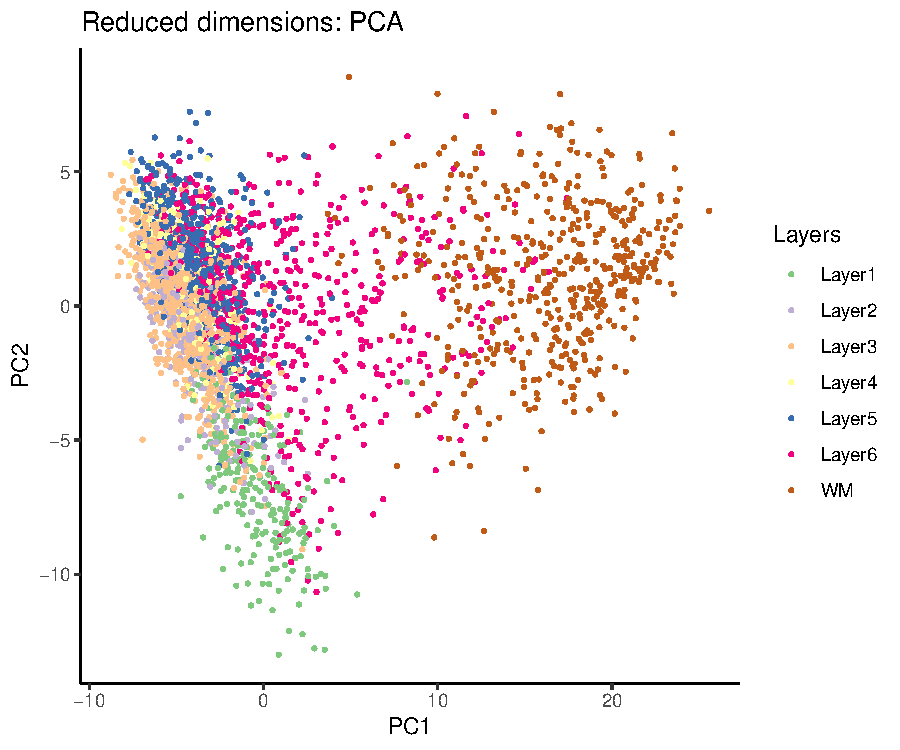
\includegraphics{_main_files/figure-latex/02_dimRed_UMAP-vis-1.pdf} 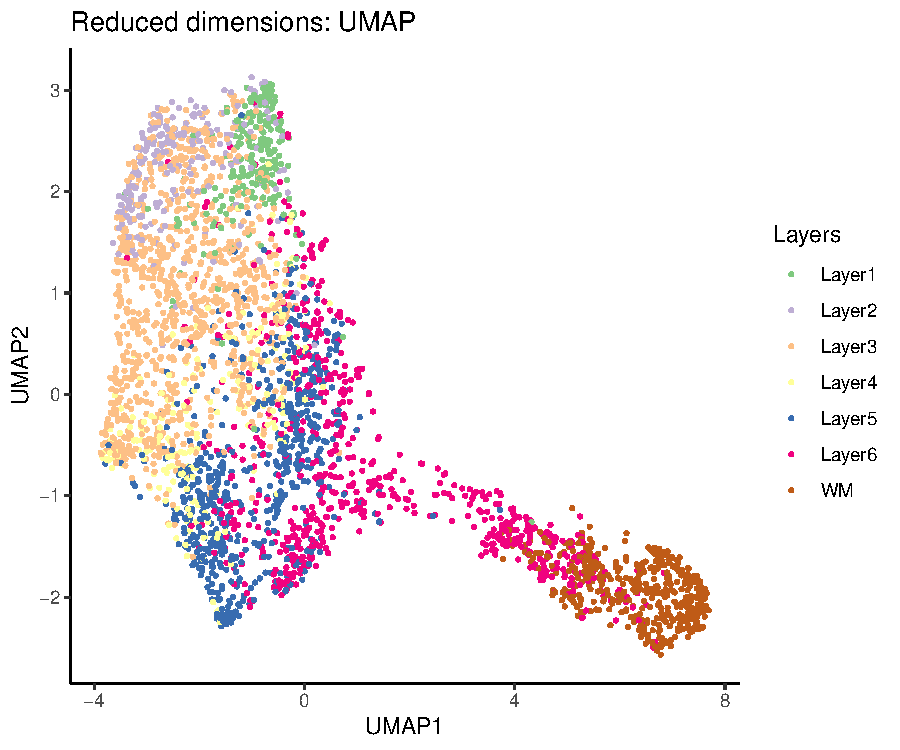
\includegraphics{_main_files/figure-latex/02_dimRed_UMAP-vis-2.pdf}

\hypertarget{clustering}{%
\section{Clustering}\label{clustering}}

\hypertarget{background-3}{%
\subsection{Background}\label{background-3}}

The clustering of observations into statistically similar groups is a well-established application in both bulk and single-cell RNA-Seq analysis. Clustering is a helpful tool because it structures and orders the data, allowing useful insights to be gained from complex, multivariate datasets and use those insights to classify the observed data or to generate hypotheses.

Common clustering methods are applied to ST data based on correlation or statistical distance of gene expression measurements. As we briefly touched above, the dimensionality of ST data means that sample distances in gene expression space tend to be small and not reliable for identifying clusters, so feature selection (gene selection) or dimensionality reduction approaches (i.e., PCA, UMAP) tend to be taken before clustering.

Common approaches to clustering gene expression data include k-means, hierarchical and Louvain algorithms, and all have been applied to the clustering of ST data. Some of these methods are implemented in some of the most popular single-cell analysis packages, such as \texttt{Seurat} \citep{Hao2021Jun} and \texttt{scran} \citep{Lun2016Oct} and have been used for clustering in a number of ST studies.

\hypertarget{clustering-on-hvgs}{%
\subsection{Clustering on HVGs}\label{clustering-on-hvgs}}

Here, we apply graph-based clustering to the top 50 PCs calculated on the set of selected HVGs, using the Walktrap method implemented in \texttt{scran} \citep{Lun2016Oct}. To do so, we assume that (i) each spot is equal to a cell and (ii) we can detect from the gene expression the biologically informative spatial distribution patterns of cell types.

\begin{Shaded}
\begin{Highlighting}[]
\DocumentationTok{\#\# Set seed}
\FunctionTok{set.seed}\NormalTok{(}\DecValTok{987}\NormalTok{)}
\DocumentationTok{\#\# Set number of Nearest{-}Neighbours (NNs)}
\NormalTok{k }\OtherTok{\textless{}{-}} \DecValTok{10}
\DocumentationTok{\#\# Build the k{-}NN graph}
\NormalTok{g }\OtherTok{\textless{}{-}} \FunctionTok{buildSNNGraph}\NormalTok{(spe, }\AttributeTok{k =}\NormalTok{ k, }\AttributeTok{use.dimred =} \StringTok{"PCA"}\NormalTok{)}
\DocumentationTok{\#\# Run walktrap clustering}
\NormalTok{g\_walk }\OtherTok{\textless{}{-}}\NormalTok{ igraph}\SpecialCharTok{::}\FunctionTok{cluster\_walktrap}\NormalTok{(g)}
\DocumentationTok{\#\# Get the cluster labels}
\NormalTok{clus }\OtherTok{\textless{}{-}}\NormalTok{ g\_walk}\SpecialCharTok{$}\NormalTok{membership}
\DocumentationTok{\#\# Check how many}
\FunctionTok{table}\NormalTok{(clus)}
\end{Highlighting}
\end{Shaded}

\begin{verbatim}
## clus
##   1   2   3   4   5   6 
## 350 354 661 895 366 885
\end{verbatim}

\begin{Shaded}
\begin{Highlighting}[]
\DocumentationTok{\#\# Store cluster labels in column \textquotesingle{}label\textquotesingle{} in colData}
\FunctionTok{colLabels}\NormalTok{(spe) }\OtherTok{\textless{}{-}} \FunctionTok{factor}\NormalTok{(clus)}
\end{Highlighting}
\end{Shaded}

\hypertarget{hvgs-clustering-visualisations}{%
\subsection{HVGs clustering visualisations}\label{hvgs-clustering-visualisations}}

We can visualise the clusters in two ways:\\
1. plotting in spatial coordinates on the tissue map
2. plotting in the UMAP/PCA embeddings.

We can use plotting functions either from the \href{https://bioconductor.org/packages/ggspavis}{ggspavis}package.

For reference, we will also display the ground truth (manually annotated) labels available for this dataset.

\begin{Shaded}
\begin{Highlighting}[]
\DocumentationTok{\#\# Plot in tissue map}
\FunctionTok{plotSpots}\NormalTok{(spe, }\AttributeTok{annotate =} \StringTok{"label"}\NormalTok{, }
          \AttributeTok{palette =} \StringTok{"libd\_layer\_colors"}\NormalTok{)}

\DocumentationTok{\#\# Plot ground truth in tissue map}
\FunctionTok{plotSpots}\NormalTok{(spe, }\AttributeTok{annotate =} \StringTok{"ground\_truth"}\NormalTok{, }
          \AttributeTok{palette =} \StringTok{"libd\_layer\_colors"}\NormalTok{)}
\end{Highlighting}
\end{Shaded}

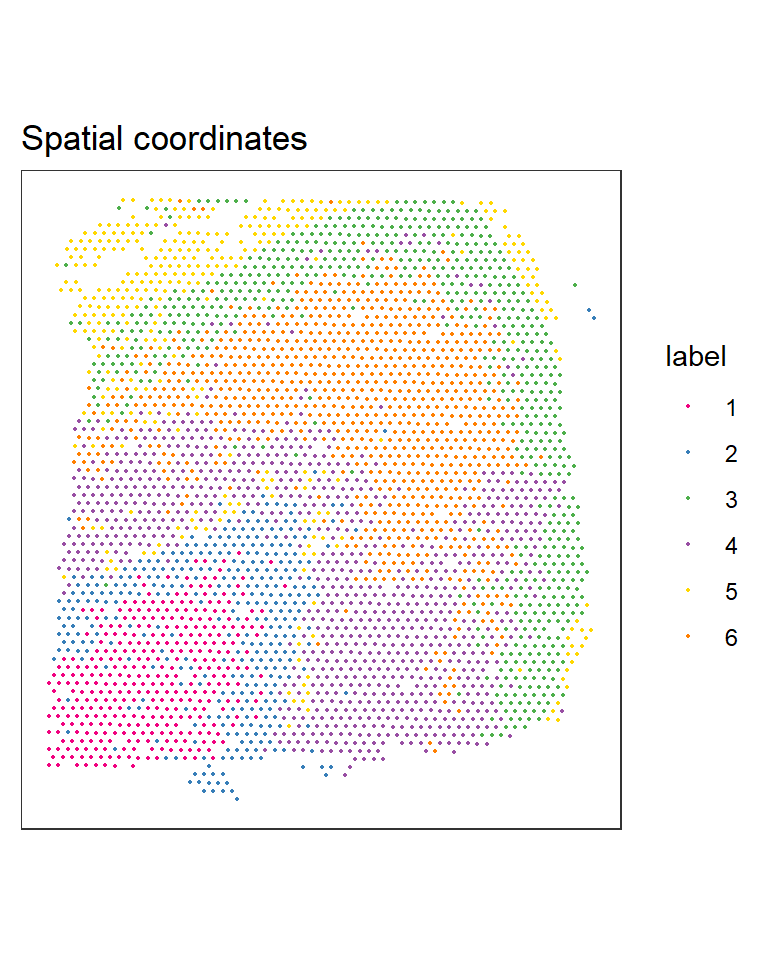
\includegraphics[width=0.5\linewidth]{_main_files/figure-latex/02_clust_vis-map-1} 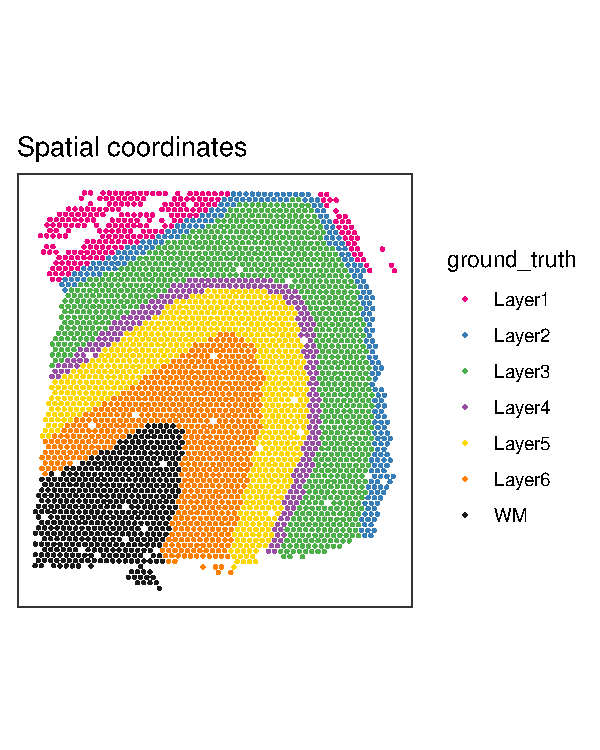
\includegraphics[width=0.5\linewidth]{_main_files/figure-latex/02_clust_vis-map-2}

\begin{Shaded}
\begin{Highlighting}[]
\DocumentationTok{\#\# Plot clusters in PCA space}
\FunctionTok{plotDimRed}\NormalTok{(spe, }\AttributeTok{type =} \StringTok{"PCA"}\NormalTok{, }
           \AttributeTok{annotate =} \StringTok{"label"}\NormalTok{, }\AttributeTok{palette =} \StringTok{"libd\_layer\_colors"}\NormalTok{)}

\DocumentationTok{\#\# Plot clusters in UMAP space}
\FunctionTok{plotDimRed}\NormalTok{(spe, }\AttributeTok{type =} \StringTok{"UMAP"}\NormalTok{, }
           \AttributeTok{annotate =} \StringTok{"label"}\NormalTok{, }\AttributeTok{palette =} \StringTok{"libd\_layer\_colors"}\NormalTok{)}
\end{Highlighting}
\end{Shaded}

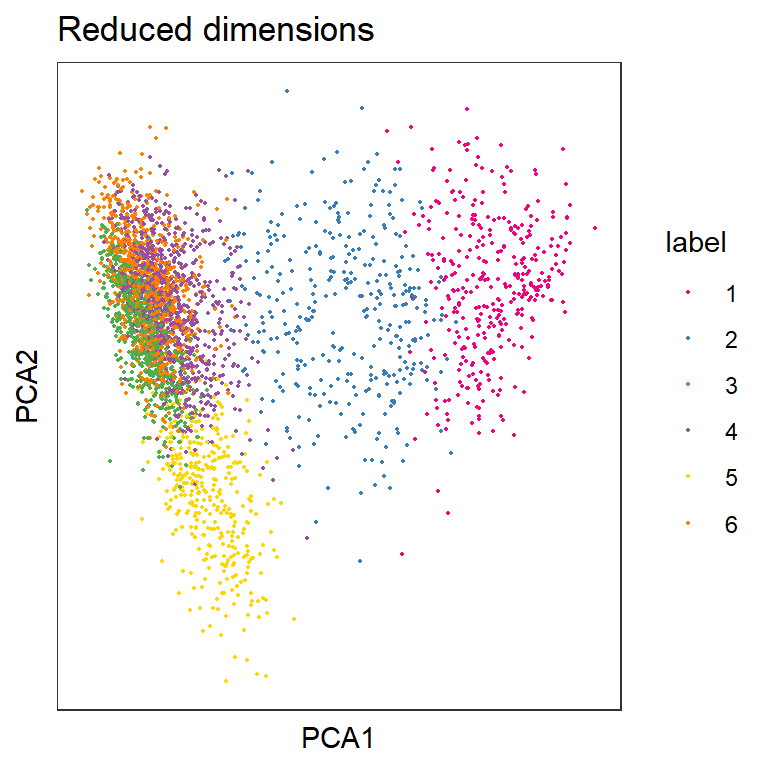
\includegraphics[width=0.5\linewidth]{_main_files/figure-latex/02_clust_vis-DimRed-1} 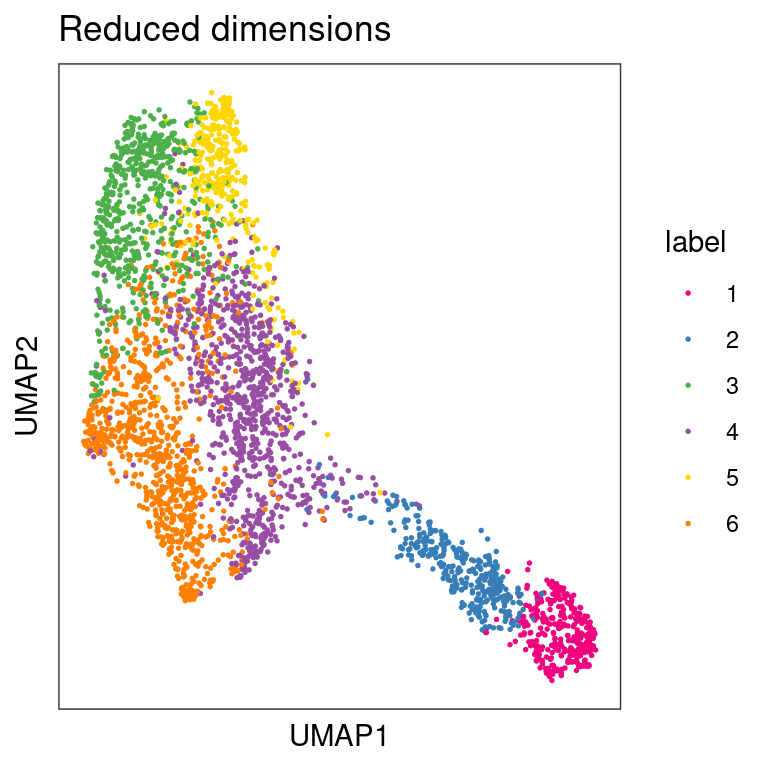
\includegraphics[width=0.5\linewidth]{_main_files/figure-latex/02_clust_vis-DimRed-2}

From the visualizations, we can see that the clustering reproduces, up to an extend, the known biological structure of the tissue, but not perfectly. One reason for this could be the fact that each spot may comprise of many different cells whose gene expression profiles are diluted in the overall profile of the spot, thus leading to low-quality clustering.

\hypertarget{spatially-aware-clustering}{%
\subsection{Spatially-aware clustering}\label{spatially-aware-clustering}}

In STx data, we can also perform clustering that takes spatial information into account, for example to identify spatially compact or spatially connected clusters.

A simple strategy is to perform graph-based clustering on a set of features (columns) that includes both molecular features (gene expression) and spatial features (x-y coordinates). In this case, a crucial tuning parameter is the relative amount of scaling between the two data modalities -- if the scaling is chosen poorly, either the molecular or spatial features will dominate the clustering. Depending on data availability, further modalities could also be included. In this section, we will include some examples on this clustering approach.

\hypertarget{inter-cluster-differentially-expressed-genes-dges}{%
\section{Inter-cluster differentially expressed genes (DGEs)}\label{inter-cluster-differentially-expressed-genes-dges}}

\hypertarget{background-4}{%
\subsection{Background}\label{background-4}}

Here, we will identify differentially expressed genes bewteen clusters.

We will use the \texttt{findMarkers} implementation from the \texttt{scran} \citep{Lun2016Oct}. This implementation uses a binomial test, which tests for genes that differ in the proportion expressed vs.~not expressed between clusters. This is a more stringent test than the default t-tests, and tends to select genes that are easier to interpret and validate experimentally.

\hypertarget{dges-identification}{%
\subsection{DGEs identification}\label{dges-identification}}

\begin{Shaded}
\begin{Highlighting}[]
\DocumentationTok{\#\# Set gene names as row names ease of plotting}
\FunctionTok{rownames}\NormalTok{(spe) }\OtherTok{\textless{}{-}} \FunctionTok{rowData}\NormalTok{(spe)}\SpecialCharTok{$}\NormalTok{gene\_name}
\DocumentationTok{\#\# Test for DGEs}
\NormalTok{markers }\OtherTok{\textless{}{-}} \FunctionTok{findMarkers}\NormalTok{(spe, }\AttributeTok{test =} \StringTok{"binom"}\NormalTok{, }\AttributeTok{direction =} \StringTok{"up"}\NormalTok{)}
\DocumentationTok{\#\# Check output}
\NormalTok{markers}
\end{Highlighting}
\end{Shaded}

\begin{verbatim}
## List of length 6
## names(6): 1 2 3 4 5 6
\end{verbatim}

The output from the \texttt{findMarkers} implementation is a list of length equal to the number of clusters. Each element of the list contains the Log-Fold-Change (LogFC) of each gene between one cluster and all others.

\hypertarget{dges-visualisation}{%
\subsection{DGEs visualisation}\label{dges-visualisation}}

Here we will plot LogFCs for cluster 1 against all other clusters

\begin{Shaded}
\begin{Highlighting}[]
\DocumentationTok{\#\# Select cluster 1 genes}
\NormalTok{interesting }\OtherTok{\textless{}{-}}\NormalTok{ markers[[}\DecValTok{1}\NormalTok{]]}
\DocumentationTok{\#\# Get the top genes}
\NormalTok{best\_set }\OtherTok{\textless{}{-}}\NormalTok{ interesting[interesting}\SpecialCharTok{$}\NormalTok{Top }\SpecialCharTok{\textless{}=} \DecValTok{5}\NormalTok{, ]}
\DocumentationTok{\#\# Calculate the effect}
\NormalTok{logFCs }\OtherTok{\textless{}{-}} \FunctionTok{getMarkerEffects}\NormalTok{(best\_set)}
\DocumentationTok{\#\# Plot a heat map}
\FunctionTok{pheatmap}\NormalTok{(logFCs, }\AttributeTok{breaks =} \FunctionTok{seq}\NormalTok{(}\SpecialCharTok{{-}}\DecValTok{5}\NormalTok{, }\DecValTok{5}\NormalTok{, }\AttributeTok{length.out =} \DecValTok{101}\NormalTok{))}
\end{Highlighting}
\end{Shaded}

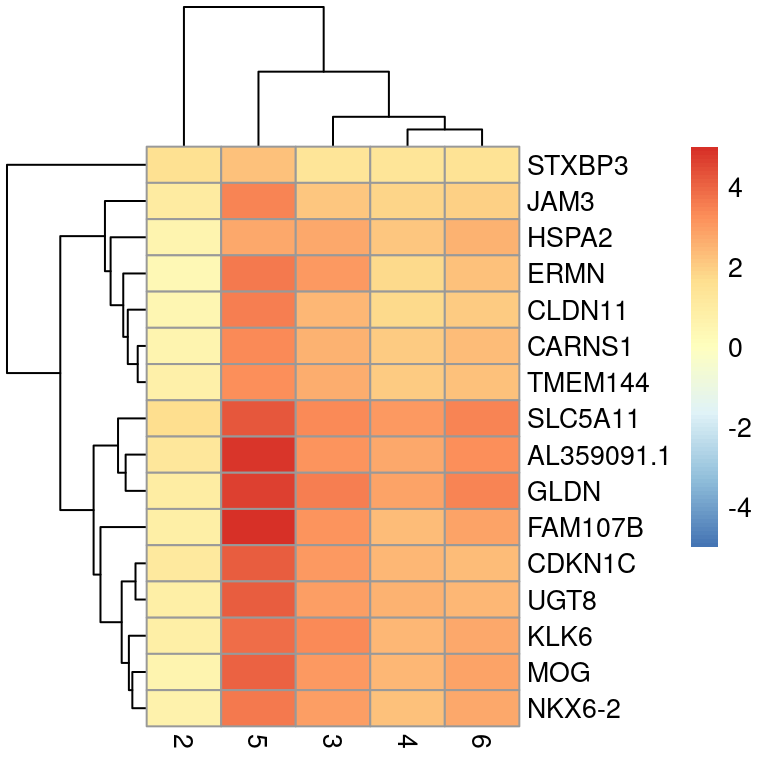
\includegraphics[width=0.5\linewidth]{_main_files/figure-latex/02_dges_vis-clst1-1}

Below we will plot the log-transformed normalised expression of the top genes for one cluster alongside their expression in the other clusters.

\begin{Shaded}
\begin{Highlighting}[]
\DocumentationTok{\#\# Select genes}
\NormalTok{top\_genes }\OtherTok{\textless{}{-}} \FunctionTok{head}\NormalTok{(}\FunctionTok{rownames}\NormalTok{(interesting))}
\DocumentationTok{\#\# Plot expression}
\FunctionTok{plotExpression}\NormalTok{(spe, }\AttributeTok{x =} \StringTok{"label"}\NormalTok{, }\AttributeTok{features =}\NormalTok{ top\_genes)}
\end{Highlighting}
\end{Shaded}

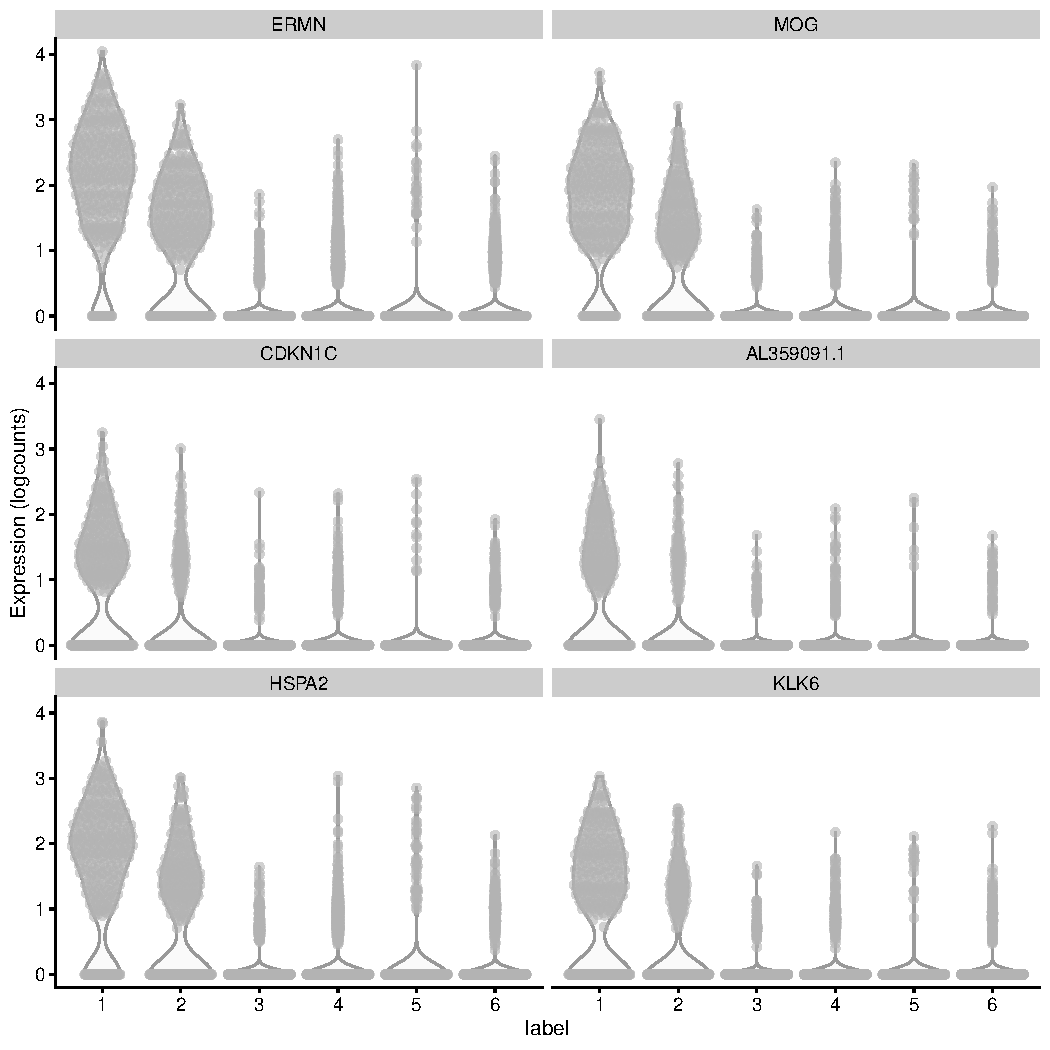
\includegraphics{_main_files/figure-latex/02_dges_vis-2-1.pdf}

\hypertarget{other-visualisations}{%
\section{Other visualisations}\label{other-visualisations}}

\hypertarget{putting-it-all-together}{%
\section{Putting it all together}\label{putting-it-all-together}}

\begin{Shaded}
\begin{Highlighting}[]
\CommentTok{\# \# clear workspace from previous chapters}
\CommentTok{\# rm(list = ls(all = TRUE))}
\CommentTok{\# }
\CommentTok{\# \# LOAD DATA}
\CommentTok{\# }
\CommentTok{\# library(SpatialExperiment)}
\CommentTok{\# library(STexampleData)}
\CommentTok{\# spe \textless{}{-} Visium\_humanDLPFC()}
\CommentTok{\# }
\CommentTok{\# \# QUALITY CONTROL (QC)}
\CommentTok{\# }
\CommentTok{\# library(scater)}
\CommentTok{\# \# subset to keep only spots over tissue}
\CommentTok{\# spe \textless{}{-} spe[, colData(spe)$in\_tissue == 1]}
\CommentTok{\# \# identify mitochondrial genes}
\CommentTok{\# is\_mito \textless{}{-} grepl("(\^{}MT{-})|(\^{}mt{-})", rowData(spe)$gene\_name)}
\CommentTok{\# \# calculate per{-}spot QC metrics}
\CommentTok{\# spe \textless{}{-} addPerCellQC(spe, subsets = list(mito = is\_mito))}
\CommentTok{\# \# select QC thresholds}
\CommentTok{\# qc\_lib\_size \textless{}{-} colData(spe)$sum \textless{} 600}
\CommentTok{\# qc\_detected \textless{}{-} colData(spe)$detected \textless{} 400}
\CommentTok{\# qc\_mito \textless{}{-} colData(spe)$subsets\_mito\_percent \textgreater{} 28}
\CommentTok{\# qc\_cell\_count \textless{}{-} colData(spe)$cell\_count \textgreater{} 10}
\CommentTok{\# \# combined set of discarded spots}
\CommentTok{\# discard \textless{}{-} qc\_lib\_size | qc\_detected | qc\_mito | qc\_cell\_count}
\CommentTok{\# colData(spe)$discard \textless{}{-} discard}
\CommentTok{\# \# filter low{-}quality spots}
\CommentTok{\# spe \textless{}{-} spe[, !colData(spe)$discard]}
\CommentTok{\# }
\CommentTok{\# \# NORMALIZATION}
\CommentTok{\# }
\CommentTok{\# library(scran)}
\CommentTok{\# \# calculate logcounts using library size factors}
\CommentTok{\# spe \textless{}{-} logNormCounts(spe)}
\CommentTok{\# }
\CommentTok{\# \# FEATURE SELECTION}
\CommentTok{\# }
\CommentTok{\# \# remove mitochondrial genes}
\CommentTok{\# spe \textless{}{-} spe[!is\_mito, ]}
\CommentTok{\# \# fit mean{-}variance relationship}
\CommentTok{\# dec \textless{}{-} modelGeneVar(spe)}
\CommentTok{\# \# select top HVGs}
\CommentTok{\# top\_hvgs \textless{}{-} getTopHVGs(dec, prop = 0.1)}
\CommentTok{\# }
\CommentTok{\# \# DIMENSIONALITY REDUCTION}
\CommentTok{\# }
\CommentTok{\# \# compute PCA}
\CommentTok{\# set.seed(123)}
\CommentTok{\# spe \textless{}{-} runPCA(spe, subset\_row = top\_hvgs)}
\CommentTok{\# \# compute UMAP on top 50 PCs}
\CommentTok{\# set.seed(123)}
\CommentTok{\# spe \textless{}{-} runUMAP(spe, dimred = "PCA")}
\CommentTok{\# \# update column names}
\CommentTok{\# colnames(reducedDim(spe, "UMAP")) \textless{}{-} paste0("UMAP", 1:2)}
\CommentTok{\# }
\CommentTok{\# \# CLUSTERING}
\CommentTok{\# }
\CommentTok{\# \# graph{-}based clustering}
\CommentTok{\# set.seed(123)}
\CommentTok{\# k \textless{}{-} 10}
\CommentTok{\# g \textless{}{-} buildSNNGraph(spe, k = k, use.dimred = "PCA")}
\CommentTok{\# g\_walk \textless{}{-} igraph::cluster\_walktrap(g)}
\CommentTok{\# clus \textless{}{-} g\_walk$membership}
\CommentTok{\# colLabels(spe) \textless{}{-} factor(clus)}
\CommentTok{\# }
\CommentTok{\# \# MARKER GENES}
\CommentTok{\# \# test for marker genes}
\CommentTok{\# rownames(spe) \textless{}{-} rowData(spe)$gene\_name}
\CommentTok{\# markers \textless{}{-} findMarkers(spe, test = "binom", direction = "up")}
\end{Highlighting}
\end{Shaded}

\hypertarget{practical-session-3}{%
\chapter{Practical session 3}\label{practical-session-3}}

This practical session will demonstrate the application of the most commonly used spatial analysis tools to STx data, and how we work with coordinate data alongside expression data. \#\# Load packages

\begin{itemize}
\item
  \href{https://cran.r-project.org/web/packages/spdep/index.html}{\texttt{spdep}} is a collection of functions to create spatial weights matrix objects from polygon \emph{`contiguities'}, from point patterns by distance and tessellations, for summarizing these objects, and for permitting their use in spatial data analysis like regional aggregation and tests for spatial \emph{`autocorrelation'}.
\item
  \href{https://cran.r-project.org/web/packages/sf/index.html}{\texttt{sf}} (\emph{Simple Features for R}) is a package that offers support for simple features, a standardized way to encode spatial vector data.
\item
  \href{https://cran.r-project.org/web/packages/GWmodel/index.html}{\texttt{GWmodel}} is a suit of models that fit situations when data are not described well by some global model, but where there are spatial regions where a suitably localised calibration provides a better description.
\end{itemize}

\hypertarget{background-5}{%
\section{Background}\label{background-5}}

\hypertarget{main-geocomputatinal-data-structures}{%
\subsection{Main geocomputatinal data structures}\label{main-geocomputatinal-data-structures}}

There are three main data structures that we need to have ready before we undertake a geocomputational approach to STx data analysis. Namely these are; (1) geometries (point and polygon), (2) neighbours lists and (3) distance matrices.

\begin{enumerate}
\def\labelenumi{\arabic{enumi}.}
\item
  Spatial geometries can be points, lines, polygons and pixels. Polygons consist of a multitude of points connected by lines and can have many forms like circle, hexagon, non-canonical polygon etc.
\item
  Neighbour lists are special types of lists that contain information about the neighbours of each polygon. The neighbours can be defined either by adjacency or by distance.
\item
  Distance matrices contain the distances between different points and can be either weighted or un-weighted. The weighted distances are usually objective to each point and its neighbours. Meaning that the closer or farther a neighbour is from the point of focus, the weight of their distance changes according to an applied kernel. Usually in the case of STx data, like the ones generated by the 10X Visium platform, the un-weighted distance between is two points is in pixels and we acquire it from the \texttt{spaceranger} output.
\end{enumerate}

\hypertarget{the-sf-objects}{%
\subsection{\texorpdfstring{The \texttt{sf} objects}{The sf objects}}\label{the-sf-objects}}

Package \texttt{sf} represents simple features as native R objects. All functions and methods in \texttt{sf} that operate on spatial data are prefixed by \emph{st\_}, which refers to \emph{spatial type}. Simple features are implemented as R native data, using simple data structures (S3 classes, lists, matrix, vector). Typical use involves reading, manipulating and writing of sets of features, with attributes and geometries.

As attributes are typically stored in \texttt{data.frame} objects (or the very similar \texttt{tbl\_df}), we will also store feature geometries in a \texttt{data.frame} column. Since geometries are not single-valued, they are put in a list-column, a list of length equal to the number of records in the \texttt{data.frame}, with each list element holding the simple feature geometry of that feature. The three classes used to represent simple features are:

\begin{itemize}
\tightlist
\item
  \texttt{sf}, the table (\texttt{data.frame}) with feature attributes and feature geometries, which contains
\item
  \texttt{sfc}, the list-column with the geometries for each feature (record), which is composed of
\item
  \texttt{sfg}, the feature geometry of an individual simple feature.
\end{itemize}

\hypertarget{simple-feature-geometry-types}{%
\subsubsection{Simple feature geometry types}\label{simple-feature-geometry-types}}

The following seven simple feature types are the most common:

\begin{longtable}[]{@{}
  >{\raggedright\arraybackslash}p{(\columnwidth - 2\tabcolsep) * \real{0.1806}}
  >{\raggedright\arraybackslash}p{(\columnwidth - 2\tabcolsep) * \real{0.8194}}@{}}
\toprule\noalign{}
\begin{minipage}[b]{\linewidth}\raggedright
type
\end{minipage} & \begin{minipage}[b]{\linewidth}\raggedright
description
\end{minipage} \\
\midrule\noalign{}
\endhead
\bottomrule\noalign{}
\endlastfoot
\texttt{POINT} & zero-dimensional geometry containing a single point \\
\texttt{LINESTRING} & sequence of points connected by straight, non-self intersecting line pieces; one-dimensional geometry \\
\texttt{POLYGON} & geometry with a positive area (two-dimensional); sequence of points form a closed, non-self intersecting ring; the first ring denotes the exterior ring, zero or more subsequent rings denote holes in this exterior ring \\
\texttt{MULTIPOINT} & set of points; a MULTIPOINT is simple if no two Points in the MULTIPOINT are equal \\
\texttt{MULTILINESTRING} & set of linestrings \\
\texttt{MULTIPOLYGON} & set of polygons \\
\texttt{GEOMETRYCOLLECTION} & set of geometries of any type except GEOMETRYCOLLECTION \\
\end{longtable}

Each of the geometry types can also be a (typed) empty set, containing zero coordinates (for \texttt{POINT} the standard is not clear how to represent the empty geometry). Empty geometries can be thought of being the analogue to missing (\texttt{NA}) attributes, NULL values or empty lists.

\hypertarget{sf-objects-with-simple-features}{%
\subsubsection{sf: objects with simple features}\label{sf-objects-with-simple-features}}

As we usually do not work with geometries of single \texttt{simple\ features}, but with datasets consisting of sets of features with attributes, the two are put together in \texttt{sf} (simple feature) objects. The following command reads a test dataset called \texttt{nc} from a file that is contained in the \texttt{sf} package:

\begin{Shaded}
\begin{Highlighting}[]
\NormalTok{nc }\OtherTok{\textless{}{-}} \FunctionTok{st\_read}\NormalTok{(}\FunctionTok{system.file}\NormalTok{(}\StringTok{"shape/nc.shp"}\NormalTok{, }\AttributeTok{package =} \StringTok{"sf"}\NormalTok{))}
\end{Highlighting}
\end{Shaded}

\begin{verbatim}
## Reading layer `nc' from data source 
##   `/Users/b9047753/Library/R/arm64/4.2/library/sf/shape/nc.shp' 
##   using driver `ESRI Shapefile'
## Simple feature collection with 100 features and 14 fields
## Geometry type: MULTIPOLYGON
## Dimension:     XY
## Bounding box:  xmin: -84.32385 ymin: 33.88199 xmax: -75.45698 ymax: 36.58965
## Geodetic CRS:  NAD27
\end{verbatim}

The short report printed gives the file name, the driver (ESRI Shapefile), mentions that there are 100 features (records, represented as rows) and 14 fields (attributes, represented as columns).

This object is of class:

\begin{Shaded}
\begin{Highlighting}[]
\FunctionTok{class}\NormalTok{(nc)}
\end{Highlighting}
\end{Shaded}

\begin{verbatim}
## [1] "sf"         "data.frame"
\end{verbatim}

meaning it extends (and ``is'' a) \texttt{data.frame}, but with a single list-column with geometries, which is held in the column with name:

\begin{Shaded}
\begin{Highlighting}[]
\FunctionTok{attr}\NormalTok{(nc, }\StringTok{"sf\_column"}\NormalTok{)}
\end{Highlighting}
\end{Shaded}

\begin{verbatim}
## [1] "geometry"
\end{verbatim}

If we print the first three features, we see their attribute values and an abridged version of the geometry

\begin{Shaded}
\begin{Highlighting}[]
\FunctionTok{print}\NormalTok{(nc[}\DecValTok{9}\SpecialCharTok{:}\DecValTok{15}\NormalTok{], }\AttributeTok{n =} \DecValTok{3}\NormalTok{)}
\end{Highlighting}
\end{Shaded}

which would give the following output:

\begin{figure}

{\centering 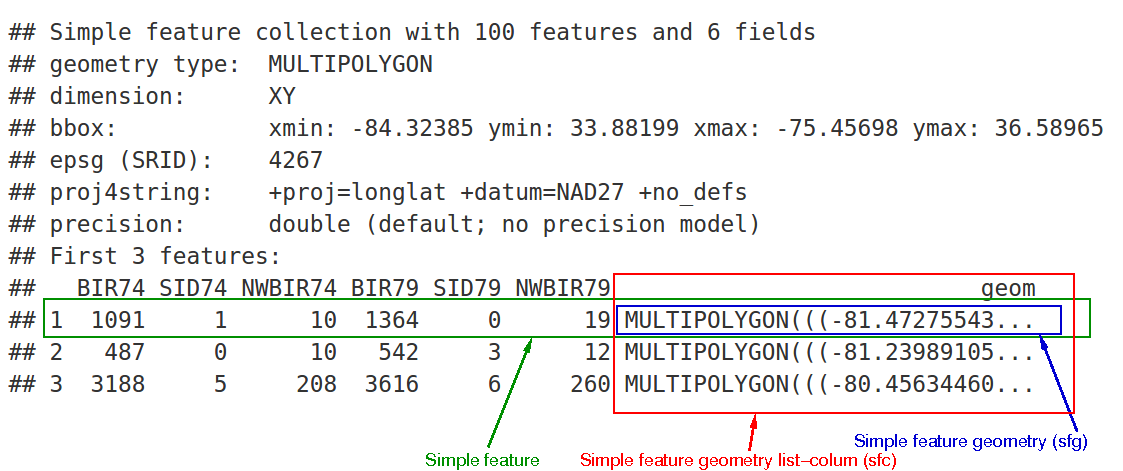
\includegraphics[width=1\linewidth]{images/sf_xfig} 

}

\caption{Overview of the `sf` object.}\label{fig:Sf-overview}
\end{figure}

In the output we see:

\begin{itemize}
\tightlist
\item
  in green a simple feature: a single record, or \texttt{data.frame} row, consisting of attributes and geometry
\item
  in blue a single simple feature geometry (an object of class \texttt{sfg})
\item
  in red a simple feature list-column (an object of class \texttt{sfc}, which is a column in the \texttt{data.frame})
\item
  that although geometries are native R objects, they are printed as \protect\hyperlink{wkb}{well-known text}
\end{itemize}

It is also possible to create \texttt{data.frame} objects with geometry list-columns that are not of class \texttt{sf}, e.g.~by:

\begin{Shaded}
\begin{Highlighting}[]
\NormalTok{nc.no\_sf }\OtherTok{\textless{}{-}} \FunctionTok{as.data.frame}\NormalTok{(nc)}
\FunctionTok{class}\NormalTok{(nc.no\_sf)}
\end{Highlighting}
\end{Shaded}

\begin{verbatim}
## [1] "data.frame"
\end{verbatim}

However, such objects:

\begin{itemize}
\tightlist
\item
  no longer register which column is the geometry list-column
\item
  no longer have a plot method, and
\item
  lack all of the other dedicated methods for class \texttt{sf}
\end{itemize}

\hypertarget{sfc-simple-feature-geometry-list-column}{%
\subsubsection{sfc: simple feature geometry list-column}\label{sfc-simple-feature-geometry-list-column}}

The column in the \texttt{sf} data.frame that contains the geometries is a list, of class \texttt{sfc}. We can retrieve the geometry list-column in this case by using standard \texttt{data.frame} notation like \texttt{nc\$geom} or \texttt{nc{[}{[}15{]}{]}}, but the more general way uses \texttt{st\_geometry}:

\begin{Shaded}
\begin{Highlighting}[]
\NormalTok{(nc\_geom }\OtherTok{\textless{}{-}} \FunctionTok{st\_geometry}\NormalTok{(nc))}
\end{Highlighting}
\end{Shaded}

\begin{verbatim}
## Geometry set for 100 features 
## Geometry type: MULTIPOLYGON
## Dimension:     XY
## Bounding box:  xmin: -84.32385 ymin: 33.88199 xmax: -75.45698 ymax: 36.58965
## Geodetic CRS:  NAD27
## First 5 geometries:
\end{verbatim}

\begin{verbatim}
## MULTIPOLYGON (((-81.47276 36.23436, -81.54084 3...
\end{verbatim}

\begin{verbatim}
## MULTIPOLYGON (((-81.23989 36.36536, -81.24069 3...
\end{verbatim}

\begin{verbatim}
## MULTIPOLYGON (((-80.45634 36.24256, -80.47639 3...
\end{verbatim}

\begin{verbatim}
## MULTIPOLYGON (((-76.00897 36.3196, -76.01735 36...
\end{verbatim}

\begin{verbatim}
## MULTIPOLYGON (((-77.21767 36.24098, -77.23461 3...
\end{verbatim}

Geometries are printed in abbreviated form, but we can view a complete geometry by selecting it, e.g.~the first one by:

\begin{Shaded}
\begin{Highlighting}[]
\NormalTok{nc\_geom[[}\DecValTok{1}\NormalTok{]]}
\end{Highlighting}
\end{Shaded}

\begin{verbatim}
## MULTIPOLYGON (((-81.47276 36.23436, -81.54084 36.27251, -81.56198 36.27359, -81.63306 36.34069, -81.74107 36.39178, -81.69828 36.47178, -81.7028 36.51934, -81.67 36.58965, -81.3453 36.57286, -81.34754 36.53791, -81.32478 36.51368, -81.31332 36.4807, -81.26624 36.43721, -81.26284 36.40504, -81.24069 36.37942, -81.23989 36.36536, -81.26424 36.35241, -81.32899 36.3635, -81.36137 36.35316, -81.36569 36.33905, -81.35413 36.29972, -81.36745 36.2787, -81.40639 36.28505, -81.41233 36.26729, -81.43104 36.26072, -81.45289 36.23959, -81.47276 36.23436)))
\end{verbatim}

The way this is printed is called \emph{well-known text}, and is part of the standards. The word \texttt{MULTIPOLYGON} is followed by three parentheses, because it can consist of multiple polygons, in the form of \texttt{MULTIPOLYGON(POL1,POL2)}, where \texttt{POL1} might consist of an exterior ring and zero or more interior rings, as of \texttt{(EXT1,HOLE1,HOLE2)}. Sets of coordinates are held together with parentheses, so we get \texttt{((crds\_ext)(crds\_hole1)(crds\_hole2))} where \texttt{crds\_} is a comma-separated set of coordinates of a ring. This leads to the case above, where \texttt{MULTIPOLYGON(((crds\_ext)))} refers to the exterior ring (1), without holes (2), of the first polygon (3) - hence three parentheses.

We can see there is a single polygon with no rings:

\begin{Shaded}
\begin{Highlighting}[]
\FunctionTok{par}\NormalTok{(}\AttributeTok{mar =} \FunctionTok{c}\NormalTok{(}\DecValTok{0}\NormalTok{,}\DecValTok{0}\NormalTok{,}\DecValTok{1}\NormalTok{,}\DecValTok{0}\NormalTok{))}
\FunctionTok{plot}\NormalTok{(nc[}\DecValTok{1}\NormalTok{], }\AttributeTok{reset =} \ConstantTok{FALSE}\NormalTok{) }\CommentTok{\# reset = FALSE: we want to add to a plot with a legend}
\FunctionTok{plot}\NormalTok{(nc[}\DecValTok{1}\NormalTok{,}\DecValTok{1}\NormalTok{], }\AttributeTok{col =} \StringTok{\textquotesingle{}grey\textquotesingle{}}\NormalTok{, }\AttributeTok{add =} \ConstantTok{TRUE}\NormalTok{)}
\end{Highlighting}
\end{Shaded}

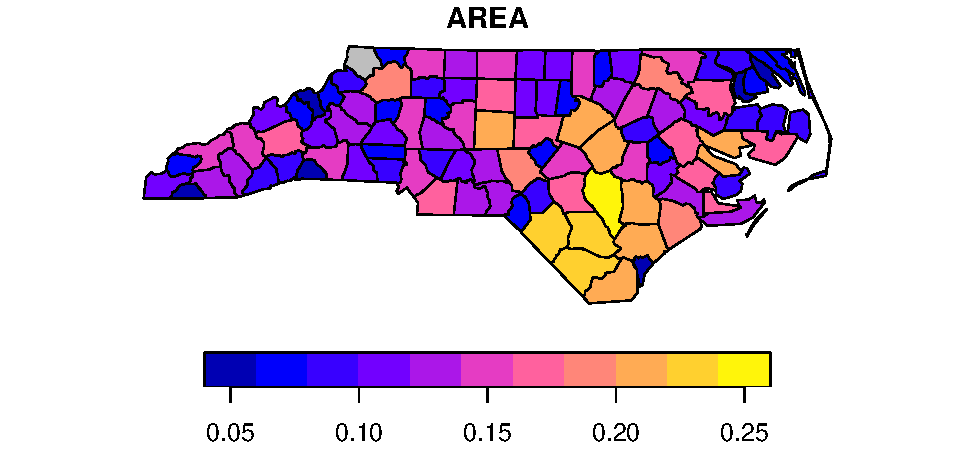
\includegraphics{_main_files/figure-latex/03_sfc_Test3-1.pdf}

Following the \texttt{MULTIPOLYGON} data structure, in R we have a list of lists of lists of matrices. For instance, we get the first 3 coordinate pairs of the second exterior ring (first ring is always exterior) for the geometry of feature 4 by:

\begin{Shaded}
\begin{Highlighting}[]
\NormalTok{nc\_geom[[}\DecValTok{4}\NormalTok{]][[}\DecValTok{2}\NormalTok{]][[}\DecValTok{1}\NormalTok{]][}\DecValTok{1}\SpecialCharTok{:}\DecValTok{3}\NormalTok{,]}
\end{Highlighting}
\end{Shaded}

\begin{verbatim}
##           [,1]     [,2]
## [1,] -76.02717 36.55672
## [2,] -75.99866 36.55665
## [3,] -75.91192 36.54253
\end{verbatim}

Geometry columns have their own class,

\begin{Shaded}
\begin{Highlighting}[]
\FunctionTok{class}\NormalTok{(nc\_geom)}
\end{Highlighting}
\end{Shaded}

\begin{verbatim}
## [1] "sfc_MULTIPOLYGON" "sfc"
\end{verbatim}

\hypertarget{sfg-simple-feature-geometry}{%
\subsubsection{sfg: simple feature geometry}\label{sfg-simple-feature-geometry}}

Simple feature geometry (\texttt{sfg}) objects carry the geometry for a single feature, e.g.~a point, linestring or polygon.

Simple feature geometries are implemented as R native data, using the following rules

\begin{enumerate}
\def\labelenumi{\arabic{enumi}.}
\tightlist
\item
  a single POINT is a numeric vector
\item
  a set of points, e.g.~in a LINESTRING or ring of a POLYGON is a \texttt{matrix}, each row containing a point
\item
  any other set is a \texttt{list}
\end{enumerate}

The below figure illustrates the different types of geometries:

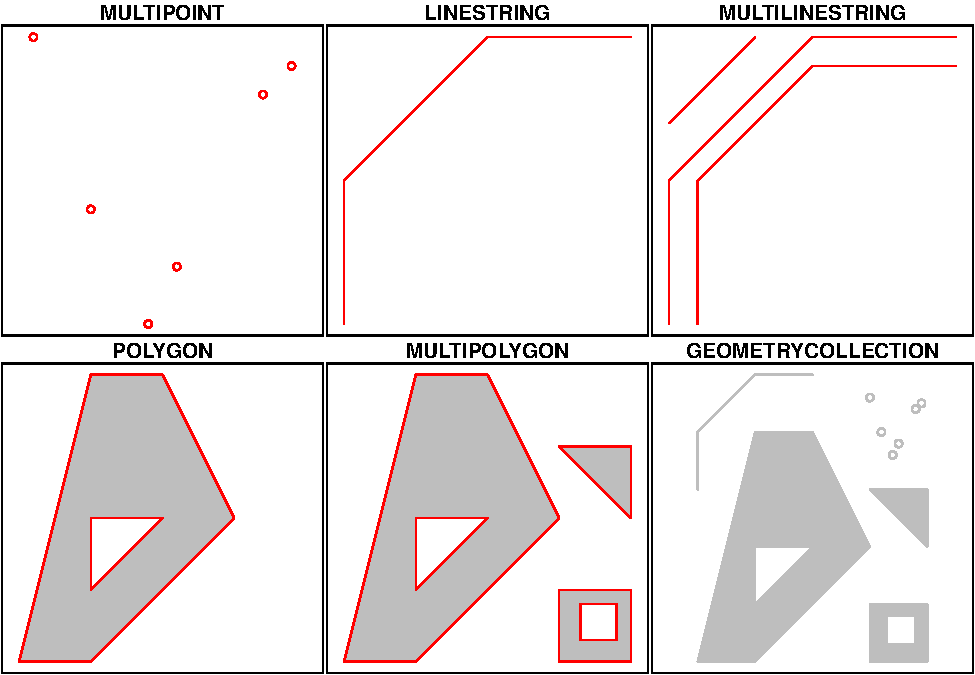
\includegraphics{_main_files/figure-latex/03_sf_Test7-1.pdf}

Geometries can also be empty, as in

\begin{Shaded}
\begin{Highlighting}[]
\NormalTok{(x }\OtherTok{\textless{}{-}} \FunctionTok{st\_geometrycollection}\NormalTok{())}
\DocumentationTok{\#\# GEOMETRYCOLLECTION EMPTY}
\FunctionTok{length}\NormalTok{(x)}
\DocumentationTok{\#\# [1] 0}
\end{Highlighting}
\end{Shaded}

\emph{The above are taken from the very well written, well-descriptive and thorough \texttt{sf} package \href{https://cran.r-project.org/web/packages/sf/vignettes/sf1.html}{vignette}.}

\hypertarget{data-structures-preparation}{%
\section{Data structures preparation}\label{data-structures-preparation}}

For this practical we will be using a human steatotic kidney dataset from the \href{https://livercellatlas.org/index.php}{Liver Atlas} \citep{GUILLIAMS2022379}. Specifically we will use the JBO019 sample.

\hypertarget{load-new-dataset}{%
\subsection{Load new dataset}\label{load-new-dataset}}

First we generate the \texttt{SpatialFeaturesExperiment} object which is an extension of the \texttt{SpatialExperiment} (SPE) object that we used in the 2nd practical session. The difference is that the SFE object has incorporated the \texttt{sf} object structure and thus can accommodate the use of geocomputational tools.

\begin{Shaded}
\begin{Highlighting}[]
\NormalTok{sampleDir }\OtherTok{\textless{}{-}} \StringTok{"./data/spaceranger\_outs/Human\_Liver\_Steatotic/JBO019\_Results"}
\NormalTok{sampleNames }\OtherTok{\textless{}{-}} \StringTok{"JBO019"}
\NormalTok{sfe }\OtherTok{\textless{}{-}} \FunctionTok{read10xVisiumSFE}\NormalTok{(}\AttributeTok{samples =}\NormalTok{ sampleDir, }
                        \AttributeTok{sample\_id =}\NormalTok{ sampleNames, }
                        \AttributeTok{type =} \StringTok{"sparse"}\NormalTok{, }
                        \AttributeTok{data =} \StringTok{"filtered"}\NormalTok{, }
                        \AttributeTok{images =} \StringTok{"lowres"}\NormalTok{, }
                        \AttributeTok{style =} \StringTok{"W"}\NormalTok{, }
                        \AttributeTok{zero.policy =} \ConstantTok{TRUE}\NormalTok{)}

\NormalTok{ground\_truth }\OtherTok{\textless{}{-}} \FunctionTok{read\_table}\NormalTok{(}\StringTok{"./data/to\_load/spotzonationGroup.txt"}\NormalTok{)}
\end{Highlighting}
\end{Shaded}

\hypertarget{spot-level-quality-control-1}{%
\section{Spot-level Quality Control}\label{spot-level-quality-control-1}}

\hypertarget{calculating-qc-metrics-1}{%
\subsection{Calculating QC metrics}\label{calculating-qc-metrics-1}}

Here we are populating the dataset with per-spot, per-gene features and geometries required to run downstream GWPCA\ldots{}

\begin{Shaded}
\begin{Highlighting}[]
\NormalTok{is\_mito }\OtherTok{\textless{}{-}} \FunctionTok{grepl}\NormalTok{(}\StringTok{"(\^{}MT{-})|(\^{}mt{-})"}\NormalTok{, }\FunctionTok{rowData}\NormalTok{(sfe)}\SpecialCharTok{$}\NormalTok{symbol)}
\NormalTok{sfe }\OtherTok{\textless{}{-}} \FunctionTok{addPerLocQC}\NormalTok{(sfe, }\AttributeTok{gTruth =}\NormalTok{ ground\_truth, }\AttributeTok{assay =} \StringTok{"counts"}\NormalTok{, }\DecValTok{2}\NormalTok{, }\AttributeTok{subsets =} \FunctionTok{list}\NormalTok{(}\AttributeTok{mito =}\NormalTok{ is\_mito))}
\NormalTok{sfe }\OtherTok{\textless{}{-}} \FunctionTok{addGeometries}\NormalTok{(sfe, }\AttributeTok{samples =}\NormalTok{ sampleDir, }\AttributeTok{sample\_id =}\NormalTok{ sampleNames, }\AttributeTok{res =} \StringTok{"fullres"}\NormalTok{)}
\NormalTok{sfe }\OtherTok{\textless{}{-}} \FunctionTok{addPerGeneQC}\NormalTok{(sfe, }\AttributeTok{assay =} \StringTok{"counts"}\NormalTok{, }\AttributeTok{version =} \ConstantTok{NULL}\NormalTok{, }\AttributeTok{mirror =} \ConstantTok{NULL}\NormalTok{)}

\FunctionTok{colData}\NormalTok{(sfe)}
\end{Highlighting}
\end{Shaded}

\begin{verbatim}
## DataFrame with 1185 rows and 15 columns
##                    in_tissue array_row array_col   sample_id            Barcode
##                    <logical> <integer> <integer> <character>        <character>
## AAACAAGTATCTCCCA-1      TRUE        50       102      JBO019 AAACAAGTATCTCCCA-1
## AAACATTTCCCGGATT-1      TRUE        61        97      JBO019 AAACATTTCCCGGATT-1
## AAACCCGAACGAAATC-1      TRUE        45       115      JBO019 AAACCCGAACGAAATC-1
## AAACGAGACGGTTGAT-1      TRUE        35        79      JBO019 AAACGAGACGGTTGAT-1
## AAACTAACGTGGCGAC-1      TRUE         8       110      JBO019 AAACTAACGTGGCGAC-1
## ...                      ...       ...       ...         ...                ...
## TTGTAATCCGTACTCG-1      TRUE        35        55      JBO019 TTGTAATCCGTACTCG-1
## TTGTGAACCTAATCCG-1      TRUE        56        90      JBO019 TTGTGAACCTAATCCG-1
## TTGTGCAGCCACGTCA-1      TRUE        60        74      JBO019 TTGTGCAGCCACGTCA-1
## TTGTGTTTCCCGAAAG-1      TRUE        51        59      JBO019 TTGTGTTTCCCGAAAG-1
## TTGTTGTGTGTCAAGA-1      TRUE        31        77      JBO019 TTGTTGTGTGTCAAGA-1
##                      Capt_area  annotation       index  sparsity       sum
##                    <character> <character> <character> <numeric> <numeric>
## AAACAAGTATCTCCCA-1           1          NA      spot_1  0.910410     13443
## AAACATTTCCCGGATT-1           1          NA      spot_2  0.967805      2648
## AAACCCGAACGAAATC-1           1         Mid      spot_3  0.864958     27733
## AAACGAGACGGTTGAT-1           1     Central      spot_4  0.835818     32973
## AAACTAACGTGGCGAC-1           1          NA      spot_5  0.995418       400
## ...                        ...         ...         ...       ...       ...
## TTGTAATCCGTACTCG-1           1          NA   spot_1181  0.933716      7612
## TTGTGAACCTAATCCG-1           1          NA   spot_1182  0.955831      4299
## TTGTGCAGCCACGTCA-1           1          NA   spot_1183  0.978252      1452
## TTGTGTTTCCCGAAAG-1           1          NA   spot_1184  0.956778      3831
## TTGTTGTGTGTCAAGA-1           1         Mid   spot_1185  0.852160     27755
##                     detected subsets_mito_sum subsets_mito_detected
##                    <integer>        <numeric>             <integer>
## AAACAAGTATCTCCCA-1      2933             1021                    12
## AAACATTTCCCGGATT-1      1054              285                    12
## AAACCCGAACGAAATC-1      4421             2087                    12
## AAACGAGACGGTTGAT-1      5375              821                    12
## AAACTAACGTGGCGAC-1       150              182                    11
## ...                      ...              ...                   ...
## TTGTAATCCGTACTCG-1      2170              733                    11
## TTGTGAACCTAATCCG-1      1446              515                    12
## TTGTGCAGCCACGTCA-1       712               54                    10
## TTGTGTTTCCCGAAAG-1      1415              422                    11
## TTGTTGTGTGTCAAGA-1      4840              906                    12
##                    subsets_mito_percent     total
##                               <numeric> <numeric>
## AAACAAGTATCTCCCA-1              7.59503     13443
## AAACATTTCCCGGATT-1             10.76284      2648
## AAACCCGAACGAAATC-1              7.52533     27733
## AAACGAGACGGTTGAT-1              2.48992     32973
## AAACTAACGTGGCGAC-1             45.50000       400
## ...                                 ...       ...
## TTGTAATCCGTACTCG-1              9.62953      7612
## TTGTGAACCTAATCCG-1             11.97953      4299
## TTGTGCAGCCACGTCA-1              3.71901      1452
## TTGTGTTTCCCGAAAG-1             11.01540      3831
## TTGTTGTGTGTCAAGA-1              3.26428     27755
\end{verbatim}

\begin{Shaded}
\begin{Highlighting}[]
\FunctionTok{rowData}\NormalTok{(sfe)}
\end{Highlighting}
\end{Shaded}

\begin{verbatim}
## DataFrame with 32738 rows and 18 columns
##                    gene_name              id       mean  detected     total
##                  <character>     <character>  <numeric> <numeric> <numeric>
## ENSG00000243485   MIR1302-10 ENSG00000243485 0.00000000  0.000000         0
## ENSG00000237613      FAM138A ENSG00000237613 0.00000000  0.000000         0
## ENSG00000186092        OR4F5 ENSG00000186092 0.00000000  0.000000         0
## ENSG00000238009 RP11-34P13.7 ENSG00000238009 0.00590717  0.590717         7
## ENSG00000239945 RP11-34P13.8 ENSG00000239945 0.00000000  0.000000         0
## ...                      ...             ...        ...       ...       ...
## ENSG00000215635   AC145205.1 ENSG00000215635          0         0         0
## ENSG00000268590        BAGE5 ENSG00000268590          0         0         0
## ENSG00000251180   CU459201.1 ENSG00000251180          0         0         0
## ENSG00000215616   AC002321.2 ENSG00000215616          0         0         0
## ENSG00000215611   AC002321.1 ENSG00000215611          0         0         0
##                 JBO019.sparsity JBO019.total JBO019.nLocations JBO019.s_min
##                       <numeric>    <numeric>         <integer>    <numeric>
## ENSG00000243485        1.000000            0                 0          Inf
## ENSG00000237613        1.000000            0                 0          Inf
## ENSG00000186092        1.000000            0                 0          Inf
## ENSG00000238009        0.994093            7                 7            1
## ENSG00000239945        1.000000            0                 0          Inf
## ...                         ...          ...               ...          ...
## ENSG00000215635               1            0                 0          Inf
## ENSG00000268590               1            0                 0          Inf
## ENSG00000251180               1            0                 0          Inf
## ENSG00000215616               1            0                 0          Inf
## ENSG00000215611               1            0                 0          Inf
##                 JBO019.max JBO019.s_mean JBO019.s_median JBO019.s_SD
##                  <numeric>     <numeric>       <numeric>   <numeric>
## ENSG00000243485          0           NaN              NA          NA
## ENSG00000237613          0           NaN              NA          NA
## ENSG00000186092          0           NaN              NA          NA
## ENSG00000238009          1             1               1           0
## ENSG00000239945          0           NaN              NA          NA
## ...                    ...           ...             ...         ...
## ENSG00000215635          0           NaN              NA          NA
## ENSG00000268590          0           NaN              NA          NA
## ENSG00000251180          0           NaN              NA          NA
## ENSG00000215616          0           NaN              NA          NA
## ENSG00000215611          0           NaN              NA          NA
##                 JBO019.p_mean JBO019.p_median JBO019.p_SD JBO019.s_CV
##                     <numeric>       <numeric>   <numeric>   <numeric>
## ENSG00000243485    0.00000000               0   0.0000000          NA
## ENSG00000237613    0.00000000               0   0.0000000          NA
## ENSG00000186092    0.00000000               0   0.0000000          NA
## ENSG00000238009    0.00590717               0   0.0766631           0
## ENSG00000239945    0.00000000               0   0.0000000          NA
## ...                       ...             ...         ...         ...
## ENSG00000215635             0               0           0          NA
## ENSG00000268590             0               0           0          NA
## ENSG00000251180             0               0           0          NA
## ENSG00000215616             0               0           0          NA
## ENSG00000215611             0               0           0          NA
##                 JBO019.p_CV
##                   <numeric>
## ENSG00000243485         NaN
## ENSG00000237613         NaN
## ENSG00000186092         NaN
## ENSG00000238009      1297.8
## ENSG00000239945         NaN
## ...                     ...
## ENSG00000215635         NaN
## ENSG00000268590         NaN
## ENSG00000251180         NaN
## ENSG00000215616         NaN
## ENSG00000215611         NaN
\end{verbatim}

\begin{Shaded}
\begin{Highlighting}[]
\FunctionTok{colGeometries}\NormalTok{(sfe)}
\end{Highlighting}
\end{Shaded}

\begin{verbatim}
## List of length 3
## names(3): spotPoly spotCntd spotHex
\end{verbatim}

\hypertarget{plot-manual-annotation}{%
\subsection{Plot manual annotation}\label{plot-manual-annotation}}

\begin{Shaded}
\begin{Highlighting}[]
\FunctionTok{ggplot}\NormalTok{() }\SpecialCharTok{+} 
  \FunctionTok{geom\_sf}\NormalTok{(}\FunctionTok{aes}\NormalTok{(}\AttributeTok{geometry =} \FunctionTok{colGeometries}\NormalTok{(sfe)}\SpecialCharTok{$}\NormalTok{spotHex}\SpecialCharTok{$}\NormalTok{geometry, }\AttributeTok{fill =} \FunctionTok{colData}\NormalTok{(sfe)}\SpecialCharTok{$}\NormalTok{annotation)) }\SpecialCharTok{+} 
  \FunctionTok{theme\_void}\NormalTok{() }\SpecialCharTok{+} 
  \FunctionTok{theme}\NormalTok{(}\AttributeTok{legend.position =} \StringTok{"right"}\NormalTok{) }\SpecialCharTok{+} 
  \FunctionTok{labs}\NormalTok{(}\AttributeTok{fill =} \StringTok{"Annotation"}\NormalTok{)}
\end{Highlighting}
\end{Shaded}

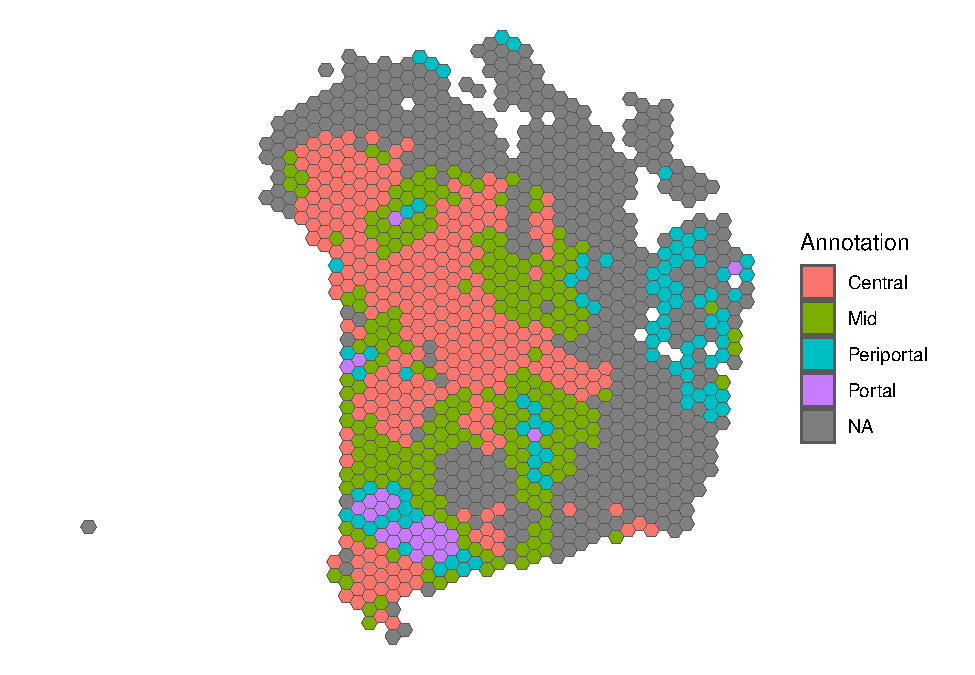
\includegraphics{_main_files/figure-latex/03_QC_sfe2-1.pdf}

\begin{Shaded}
\begin{Highlighting}[]
\CommentTok{\# \textgreater{}\textgreater{}\textgreater{}\textgreater{}\textgreater{}\textgreater{}\textgreater{}\textgreater{}\textgreater{}possible break point to continue on Pract 4\textless{}\textless{}\textless{}\textless{}\textless{}\textless{}\textless{}\textless{}\textless{}\textless{}\textless{}\textless{}\textless{}\textless{}\textless{} \#}

\CommentTok{\# Above we load the data and calculate some statistics, generate some }
\CommentTok{\# neighbour graphs and we can explore the data structures. Below we }
\CommentTok{\# apply the QC.}

\CommentTok{\# There is a catch in the above. The get.spatialNeighGraphs is going to be used}
\CommentTok{\# here to showcase the neighbour graphs but actually it is better to be called }
\CommentTok{\# after we remove unwanted locations through QC application}

\CommentTok{\# Ensembl version 92 does not match the dataset. Need to find out which}
\CommentTok{\# ensembl version they used with SpaceRanger. Otherwise some genes will not have}
\CommentTok{\# proper annotation.}

\CommentTok{\# \textgreater{}\textgreater{}\textgreater{}\textgreater{}\textgreater{}\textgreater{}\textgreater{}\textgreater{}\textgreater{}possible break point to continue on Pract 4\textless{}\textless{}\textless{}\textless{}\textless{}\textless{}\textless{}\textless{}\textless{}\textless{}\textless{}\textless{}\textless{}\textless{}\textless{} \#}
\end{Highlighting}
\end{Shaded}

\hypertarget{library-size-threshold}{%
\subsection{Library size threshold}\label{library-size-threshold}}

\begin{Shaded}
\begin{Highlighting}[]
\CommentTok{\# {-}{-}{-}{-}{-}{-}{-}{-}{-}{-}{-}{-}{-}{-}{-}{-}{-}{-}{-}{-}{-}{-}{-}{-}{-}{-}{-}{-}{-}{-}{-}{-}{-}{-}{-}{-}{-}{-}{-}{-}{-}{-}{-}{-}{-}{-}{-} \#}
\DocumentationTok{\#\# Density and histogram of library sizes}
\FunctionTok{ggplot}\NormalTok{(}\AttributeTok{data =} \FunctionTok{as.data.frame}\NormalTok{(}\FunctionTok{colData}\NormalTok{(sfe)),}
       \FunctionTok{aes}\NormalTok{(}\AttributeTok{x =}\NormalTok{ sum)) }\SpecialCharTok{+}
    \FunctionTok{geom\_histogram}\NormalTok{(}\FunctionTok{aes}\NormalTok{(}\AttributeTok{y =} \FunctionTok{after\_stat}\NormalTok{(density)), }
                   \AttributeTok{colour =} \StringTok{"black"}\NormalTok{, }
                   \AttributeTok{fill =} \StringTok{"grey"}\NormalTok{,}
                   \AttributeTok{bins =} \DecValTok{50}\NormalTok{) }\SpecialCharTok{+}
    \FunctionTok{geom\_density}\NormalTok{(}\AttributeTok{alpha =} \FloatTok{0.5}\NormalTok{,}
                 \AttributeTok{adjust =} \FloatTok{0.5}\NormalTok{,}
                 \AttributeTok{fill =} \StringTok{"\#A0CBE8"}\NormalTok{,}
                 \AttributeTok{colour =} \StringTok{"\#4E79A7"}\NormalTok{) }\SpecialCharTok{+}
    \FunctionTok{geom\_vline}\NormalTok{(}\AttributeTok{xintercept =} \FunctionTok{c}\NormalTok{(}\DecValTok{1000}\NormalTok{, }\ConstantTok{NA}\NormalTok{),}
               \AttributeTok{colour =} \StringTok{"red"}\NormalTok{, }
               \AttributeTok{linetype =} \StringTok{"dashed"}\NormalTok{) }\SpecialCharTok{+} 
    \FunctionTok{scale\_x\_continuous}\NormalTok{(}\AttributeTok{breaks =}\NormalTok{ scales}\SpecialCharTok{::}\FunctionTok{pretty\_breaks}\NormalTok{(}\AttributeTok{n =} \DecValTok{10}\NormalTok{)) }\SpecialCharTok{+} 
    \FunctionTok{scale\_y\_continuous}\NormalTok{(}\AttributeTok{breaks =}\NormalTok{ scales}\SpecialCharTok{::}\FunctionTok{pretty\_breaks}\NormalTok{(}\AttributeTok{n =} \DecValTok{10}\NormalTok{)) }\SpecialCharTok{+} 
    \FunctionTok{xlab}\NormalTok{(}\StringTok{"Library size"}\NormalTok{) }\SpecialCharTok{+} 
    \FunctionTok{ylab}\NormalTok{(}\StringTok{"Density"}\NormalTok{) }\SpecialCharTok{+} 
    \FunctionTok{theme\_classic}\NormalTok{()}
\end{Highlighting}
\end{Shaded}

\begin{verbatim}
## Warning: Removed 1 rows containing missing values (`geom_vline()`).
\end{verbatim}

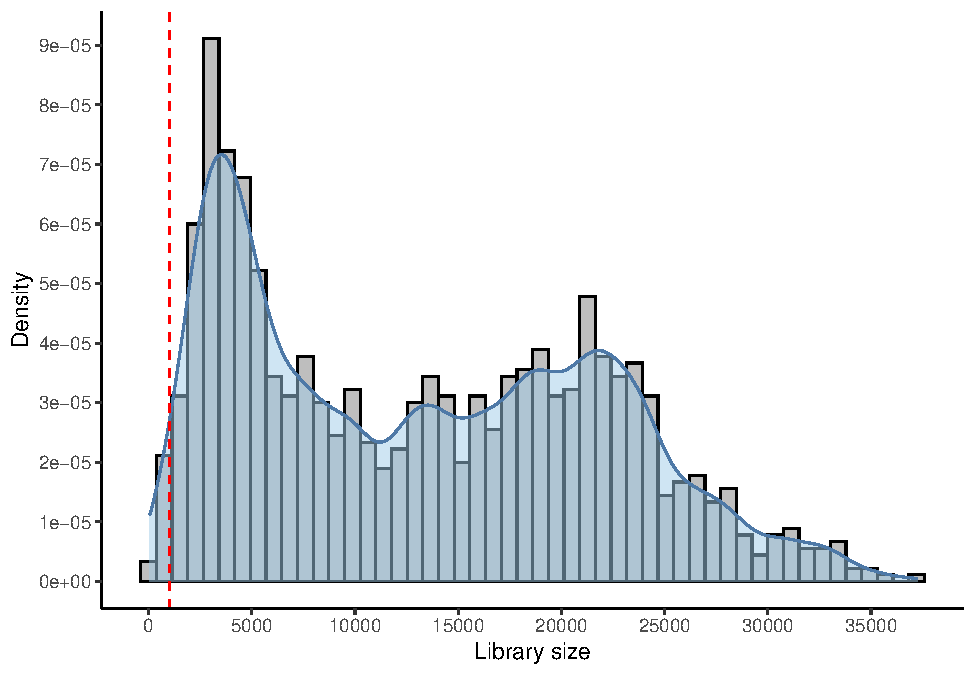
\includegraphics{_main_files/figure-latex/03_QC_sfe3-1.pdf}

\begin{Shaded}
\begin{Highlighting}[]
\DocumentationTok{\#\# Select library size threshold}
\NormalTok{qc\_lib\_size }\OtherTok{\textless{}{-}} \FunctionTok{colData}\NormalTok{(sfe)}\SpecialCharTok{$}\NormalTok{sum }\SpecialCharTok{\textless{}} \DecValTok{1000} \CommentTok{\#| colData(sfe)$sum \textgreater{} 45000}
\DocumentationTok{\#\# Check how many spots are filtered out}
\FunctionTok{table}\NormalTok{(qc\_lib\_size)}
\end{Highlighting}
\end{Shaded}

\begin{verbatim}
## qc_lib_size
## FALSE  TRUE 
##  1166    19
\end{verbatim}

\begin{Shaded}
\begin{Highlighting}[]
\DocumentationTok{\#\# Add threshold in colData}
\FunctionTok{colData}\NormalTok{(sfe)}\SpecialCharTok{$}\NormalTok{qc\_lib\_size }\OtherTok{\textless{}{-}}\NormalTok{ qc\_lib\_size}
\DocumentationTok{\#\# Check putative spatial patterns of removed spots}
\FunctionTok{ggplot}\NormalTok{() }\SpecialCharTok{+} 
    \FunctionTok{geom\_sf}\NormalTok{(}\AttributeTok{data =} \FunctionTok{colGeometry}\NormalTok{(sfe, }\StringTok{"spotHex"}\NormalTok{),}
            \FunctionTok{aes}\NormalTok{(}\AttributeTok{geometry =}\NormalTok{ geometry)) }\SpecialCharTok{+} 
    \FunctionTok{geom\_sf}\NormalTok{(}\AttributeTok{data =} \FunctionTok{colGeometry}\NormalTok{(sfe, }\StringTok{"spotHex"}\NormalTok{),}
            \FunctionTok{aes}\NormalTok{(}\AttributeTok{geometry =}\NormalTok{ geometry, }\AttributeTok{fill =} \FunctionTok{colData}\NormalTok{(sfe)}\SpecialCharTok{$}\NormalTok{qc\_lib\_size)) }\SpecialCharTok{+}
    \FunctionTok{scale\_fill\_manual}\NormalTok{(}\AttributeTok{values =} \FunctionTok{c}\NormalTok{(}\StringTok{"grey95"}\NormalTok{, }\StringTok{"red"}\NormalTok{)) }\SpecialCharTok{+} 
    \FunctionTok{labs}\NormalTok{(}\AttributeTok{fill =} \StringTok{"Discarded"}\NormalTok{) }\SpecialCharTok{+} 
    \FunctionTok{theme\_bw}\NormalTok{()}
\end{Highlighting}
\end{Shaded}

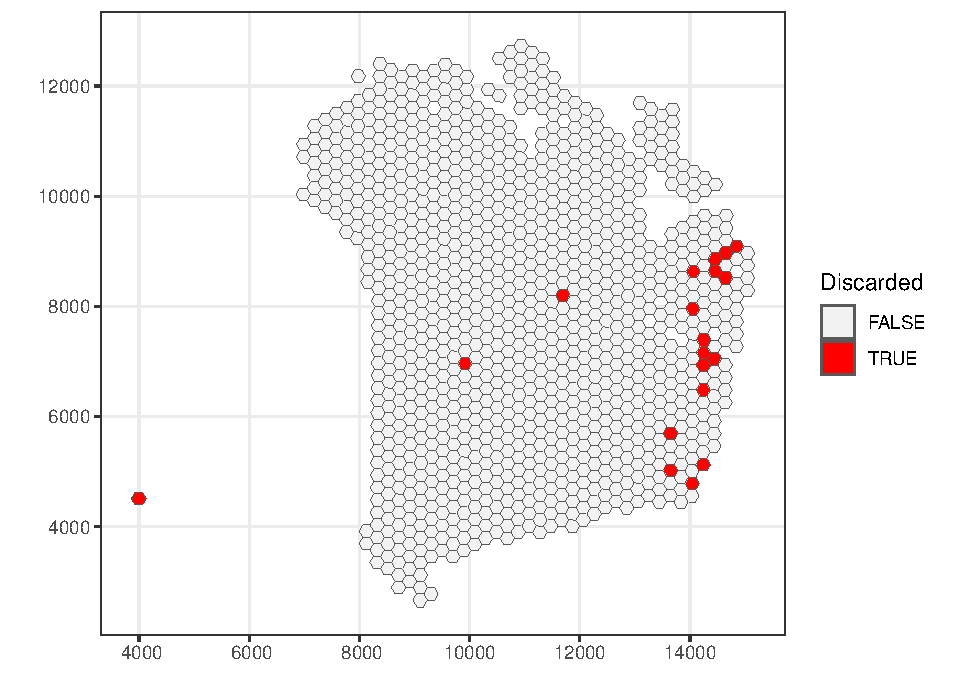
\includegraphics{_main_files/figure-latex/03_QC_sfe3-2.pdf}

\hypertarget{number-of-expressed-genes-1}{%
\subsection{Number of expressed genes}\label{number-of-expressed-genes-1}}

\begin{Shaded}
\begin{Highlighting}[]
\CommentTok{\# {-}{-}{-}{-}{-}{-}{-}{-}{-}{-}{-}{-}{-}{-}{-}{-}{-}{-}{-}{-}{-}{-}{-}{-}{-}{-}{-}{-}{-}{-}{-}{-}{-}{-}{-}{-}{-}{-}{-}{-}{-}{-}{-}{-}{-}{-}{-} \#}
\DocumentationTok{\#\# Density and histogram of expressed genes}
\FunctionTok{ggplot}\NormalTok{(}\AttributeTok{data =} \FunctionTok{as.data.frame}\NormalTok{(}\FunctionTok{colData}\NormalTok{(sfe)),}
       \FunctionTok{aes}\NormalTok{(}\AttributeTok{x =}\NormalTok{ detected)) }\SpecialCharTok{+}
    \FunctionTok{geom\_histogram}\NormalTok{(}\FunctionTok{aes}\NormalTok{(}\AttributeTok{y =} \FunctionTok{after\_stat}\NormalTok{(density)), }
                   \AttributeTok{colour =} \StringTok{"black"}\NormalTok{, }
                   \AttributeTok{fill =} \StringTok{"grey"}\NormalTok{,}
                   \AttributeTok{bins =} \DecValTok{50}\NormalTok{) }\SpecialCharTok{+}
    \FunctionTok{geom\_density}\NormalTok{(}\AttributeTok{alpha =} \FloatTok{0.5}\NormalTok{,}
                 \AttributeTok{adjust =} \FloatTok{0.5}\NormalTok{,}
                 \AttributeTok{fill =} \StringTok{"\#A0CBE8"}\NormalTok{,}
                 \AttributeTok{colour =} \StringTok{"\#4E79A7"}\NormalTok{) }\SpecialCharTok{+} 
    \FunctionTok{geom\_vline}\NormalTok{(}\AttributeTok{xintercept =} \FunctionTok{c}\NormalTok{(}\DecValTok{550}\NormalTok{, }\ConstantTok{NA}\NormalTok{),}
               \AttributeTok{colour =} \StringTok{"red"}\NormalTok{, }
               \AttributeTok{linetype =} \StringTok{"dashed"}\NormalTok{) }\SpecialCharTok{+}
    \FunctionTok{scale\_x\_continuous}\NormalTok{(}\AttributeTok{breaks =}\NormalTok{ scales}\SpecialCharTok{::}\FunctionTok{pretty\_breaks}\NormalTok{(}\AttributeTok{n =} \DecValTok{10}\NormalTok{)) }\SpecialCharTok{+} 
    \FunctionTok{scale\_y\_continuous}\NormalTok{(}\AttributeTok{breaks =}\NormalTok{ scales}\SpecialCharTok{::}\FunctionTok{pretty\_breaks}\NormalTok{(}\AttributeTok{n =} \DecValTok{10}\NormalTok{)) }\SpecialCharTok{+} 
    \FunctionTok{xlab}\NormalTok{(}\StringTok{"Genes expressed in each spot"}\NormalTok{) }\SpecialCharTok{+} 
    \FunctionTok{ylab}\NormalTok{(}\StringTok{"Density"}\NormalTok{) }\SpecialCharTok{+} 
    \FunctionTok{theme\_classic}\NormalTok{()}
\end{Highlighting}
\end{Shaded}

\begin{verbatim}
## Warning: Removed 1 rows containing missing values (`geom_vline()`).
\end{verbatim}

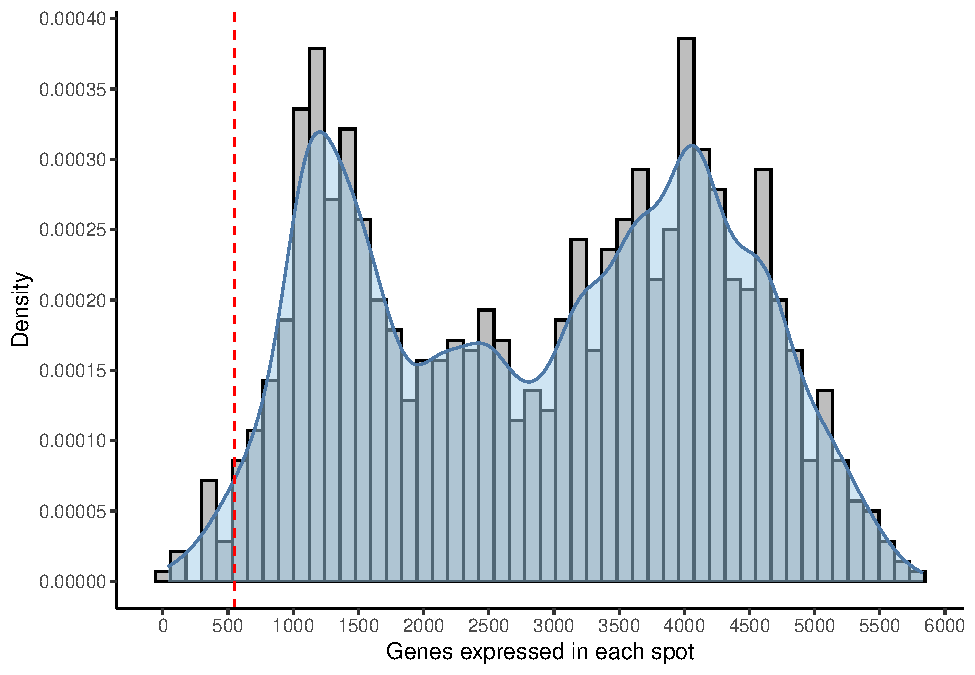
\includegraphics{_main_files/figure-latex/03_QC_sfe4-1.pdf}

\begin{Shaded}
\begin{Highlighting}[]
\DocumentationTok{\#\# Select expressed genes threshold}
\NormalTok{qc\_detected }\OtherTok{\textless{}{-}} \FunctionTok{colData}\NormalTok{(sfe)}\SpecialCharTok{$}\NormalTok{detected }\SpecialCharTok{\textless{}} \DecValTok{550} \CommentTok{\#| colData(sfe)$detected \textgreater{} 6000}
\DocumentationTok{\#\# Check how many spots are filtered out}
\FunctionTok{table}\NormalTok{(qc\_detected)}
\end{Highlighting}
\end{Shaded}

\begin{verbatim}
## qc_detected
## FALSE  TRUE 
##  1165    20
\end{verbatim}

\begin{Shaded}
\begin{Highlighting}[]
\DocumentationTok{\#\# Add threshold in colData}
\FunctionTok{colData}\NormalTok{(sfe)}\SpecialCharTok{$}\NormalTok{qc\_detected }\OtherTok{\textless{}{-}}\NormalTok{ qc\_detected}
\DocumentationTok{\#\# Check for putative spatial pattern of removed spots}
\FunctionTok{ggplot}\NormalTok{() }\SpecialCharTok{+} 
    \FunctionTok{geom\_sf}\NormalTok{(}\AttributeTok{data =} \FunctionTok{colGeometry}\NormalTok{(sfe, }\StringTok{"spotHex"}\NormalTok{),}
            \FunctionTok{aes}\NormalTok{(}\AttributeTok{geometry =}\NormalTok{ geometry)) }\SpecialCharTok{+} 
    \FunctionTok{geom\_sf}\NormalTok{(}\AttributeTok{data =} \FunctionTok{colGeometry}\NormalTok{(sfe, }\StringTok{"spotHex"}\NormalTok{),}
            \FunctionTok{aes}\NormalTok{(}\AttributeTok{geometry =}\NormalTok{ geometry, }\AttributeTok{fill =} \FunctionTok{colData}\NormalTok{(sfe)}\SpecialCharTok{$}\NormalTok{qc\_detected)) }\SpecialCharTok{+}
    \FunctionTok{scale\_fill\_manual}\NormalTok{(}\AttributeTok{values =} \FunctionTok{c}\NormalTok{(}\StringTok{"grey95"}\NormalTok{, }\StringTok{"red"}\NormalTok{)) }\SpecialCharTok{+} 
    \FunctionTok{labs}\NormalTok{(}\AttributeTok{fill =} \StringTok{"Discarded"}\NormalTok{) }\SpecialCharTok{+} 
    \FunctionTok{theme\_bw}\NormalTok{()}
\end{Highlighting}
\end{Shaded}

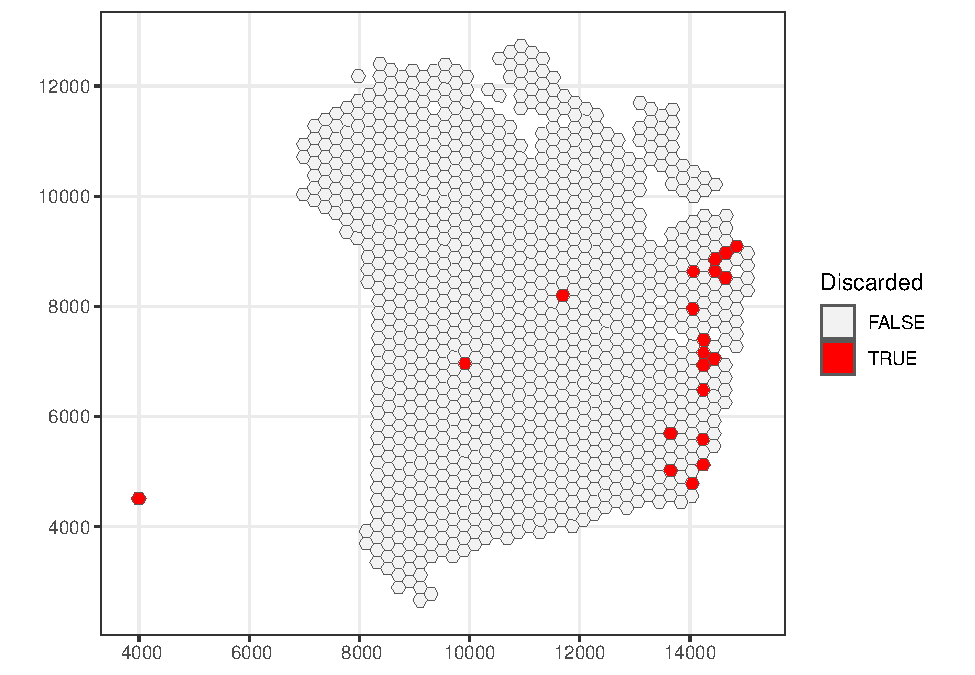
\includegraphics{_main_files/figure-latex/03_QC_sfe4-2.pdf}

\hypertarget{percentage-of-mitochondrial-expression-1}{%
\subsection{Percentage of mitochondrial expression}\label{percentage-of-mitochondrial-expression-1}}

\begin{Shaded}
\begin{Highlighting}[]
\CommentTok{\# {-}{-}{-}{-}{-}{-}{-}{-}{-}{-}{-}{-}{-}{-}{-}{-}{-}{-}{-}{-}{-}{-}{-}{-}{-}{-}{-}{-}{-}{-}{-}{-}{-}{-}{-}{-}{-}{-}{-}{-}{-}{-}{-}{-}{-}{-}{-} \#}
\DocumentationTok{\#\# Density and histogram of percentage of mitochondrial expression}
\FunctionTok{ggplot}\NormalTok{(}\AttributeTok{data =} \FunctionTok{as.data.frame}\NormalTok{(}\FunctionTok{colData}\NormalTok{(sfe)),}
       \FunctionTok{aes}\NormalTok{(}\AttributeTok{x =}\NormalTok{ subsets\_mito\_percent)) }\SpecialCharTok{+}
    \FunctionTok{geom\_histogram}\NormalTok{(}\FunctionTok{aes}\NormalTok{(}\AttributeTok{y =} \FunctionTok{after\_stat}\NormalTok{(density)), }
                   \AttributeTok{colour =} \StringTok{"black"}\NormalTok{, }
                   \AttributeTok{fill =} \StringTok{"grey"}\NormalTok{,}
                   \AttributeTok{bins =} \DecValTok{50}\NormalTok{) }\SpecialCharTok{+}
    \FunctionTok{geom\_density}\NormalTok{(}\AttributeTok{alpha =} \FloatTok{0.5}\NormalTok{,}
                 \AttributeTok{adjust =} \FloatTok{0.5}\NormalTok{,}
                 \AttributeTok{fill =} \StringTok{"\#A0CBE8"}\NormalTok{,}
                 \AttributeTok{colour =} \StringTok{"\#4E79A7"}\NormalTok{) }\SpecialCharTok{+} 
    \FunctionTok{geom\_vline}\NormalTok{(}\AttributeTok{xintercept =} \FunctionTok{c}\NormalTok{(}\DecValTok{22}\NormalTok{, }\ConstantTok{NA}\NormalTok{),}
               \AttributeTok{colour =} \StringTok{"red"}\NormalTok{, }
               \AttributeTok{linetype =} \StringTok{"dashed"}\NormalTok{) }\SpecialCharTok{+}
    \FunctionTok{scale\_x\_continuous}\NormalTok{(}\AttributeTok{breaks =}\NormalTok{ scales}\SpecialCharTok{::}\FunctionTok{pretty\_breaks}\NormalTok{(}\AttributeTok{n =} \DecValTok{10}\NormalTok{)) }\SpecialCharTok{+} 
    \FunctionTok{scale\_y\_continuous}\NormalTok{(}\AttributeTok{breaks =}\NormalTok{ scales}\SpecialCharTok{::}\FunctionTok{pretty\_breaks}\NormalTok{(}\AttributeTok{n =} \DecValTok{10}\NormalTok{)) }\SpecialCharTok{+} 
    \FunctionTok{xlab}\NormalTok{(}\StringTok{"Percentage of mitochondrial expression"}\NormalTok{) }\SpecialCharTok{+} 
    \FunctionTok{ylab}\NormalTok{(}\StringTok{"Density"}\NormalTok{) }\SpecialCharTok{+} 
    \FunctionTok{theme\_classic}\NormalTok{()}
\end{Highlighting}
\end{Shaded}

\begin{verbatim}
## Warning: Removed 1 rows containing missing values (`geom_vline()`).
\end{verbatim}

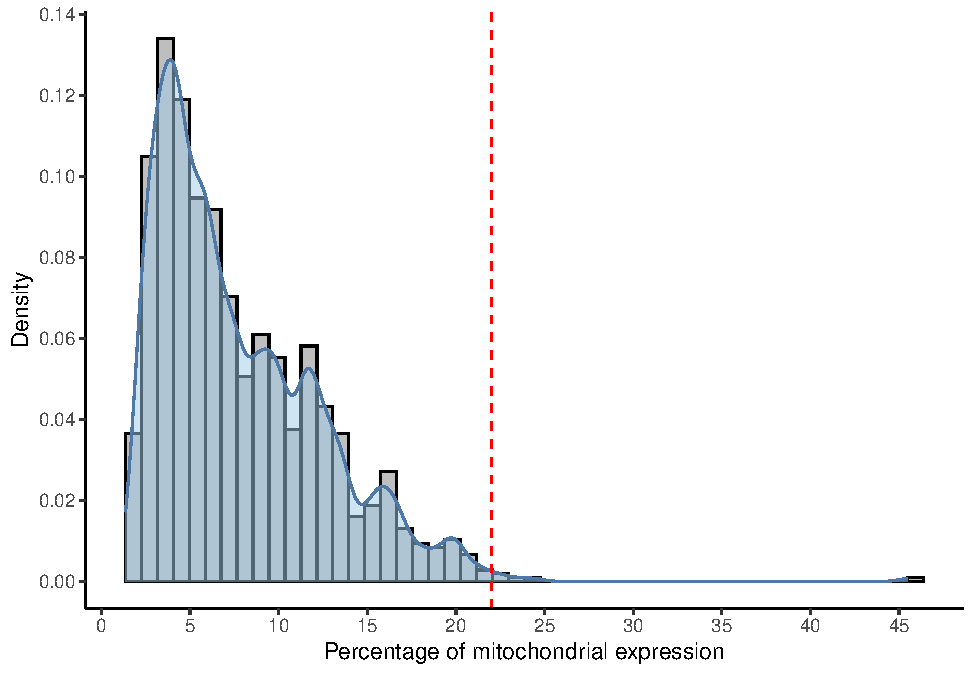
\includegraphics{_main_files/figure-latex/03_QC_sfe5-1.pdf}

\begin{Shaded}
\begin{Highlighting}[]
\DocumentationTok{\#\# Select mitochondrial percentage threshold}
\NormalTok{qc\_mito }\OtherTok{\textless{}{-}} \FunctionTok{colData}\NormalTok{(sfe)}\SpecialCharTok{$}\NormalTok{subsets\_mito\_percent }\SpecialCharTok{\textgreater{}} \DecValTok{22}
\DocumentationTok{\#\# Check how many spots are filtered out}
\FunctionTok{table}\NormalTok{(qc\_mito)}
\end{Highlighting}
\end{Shaded}

\begin{verbatim}
## qc_mito
## FALSE  TRUE 
##  1180     5
\end{verbatim}

\begin{Shaded}
\begin{Highlighting}[]
\DocumentationTok{\#\# Add threshold in colData}
\FunctionTok{colData}\NormalTok{(sfe)}\SpecialCharTok{$}\NormalTok{qc\_mito }\OtherTok{\textless{}{-}}\NormalTok{ qc\_mito}
\DocumentationTok{\#\# Check for putative spatial pattern of removed spots}
\FunctionTok{ggplot}\NormalTok{() }\SpecialCharTok{+} 
    \FunctionTok{geom\_sf}\NormalTok{(}\AttributeTok{data =} \FunctionTok{colGeometry}\NormalTok{(sfe, }\StringTok{"spotHex"}\NormalTok{),}
            \FunctionTok{aes}\NormalTok{(}\AttributeTok{geometry =}\NormalTok{ geometry)) }\SpecialCharTok{+} 
    \FunctionTok{geom\_sf}\NormalTok{(}\AttributeTok{data =} \FunctionTok{colGeometry}\NormalTok{(sfe, }\StringTok{"spotHex"}\NormalTok{),}
            \FunctionTok{aes}\NormalTok{(}\AttributeTok{geometry =}\NormalTok{ geometry, }\AttributeTok{fill =} \FunctionTok{colData}\NormalTok{(sfe)}\SpecialCharTok{$}\NormalTok{qc\_mito)) }\SpecialCharTok{+}
    \FunctionTok{scale\_fill\_manual}\NormalTok{(}\AttributeTok{values =} \FunctionTok{c}\NormalTok{(}\StringTok{"grey95"}\NormalTok{, }\StringTok{"red"}\NormalTok{)) }\SpecialCharTok{+} 
    \FunctionTok{labs}\NormalTok{(}\AttributeTok{fill =} \StringTok{"Discarded"}\NormalTok{) }\SpecialCharTok{+} 
    \FunctionTok{theme\_bw}\NormalTok{()}
\end{Highlighting}
\end{Shaded}

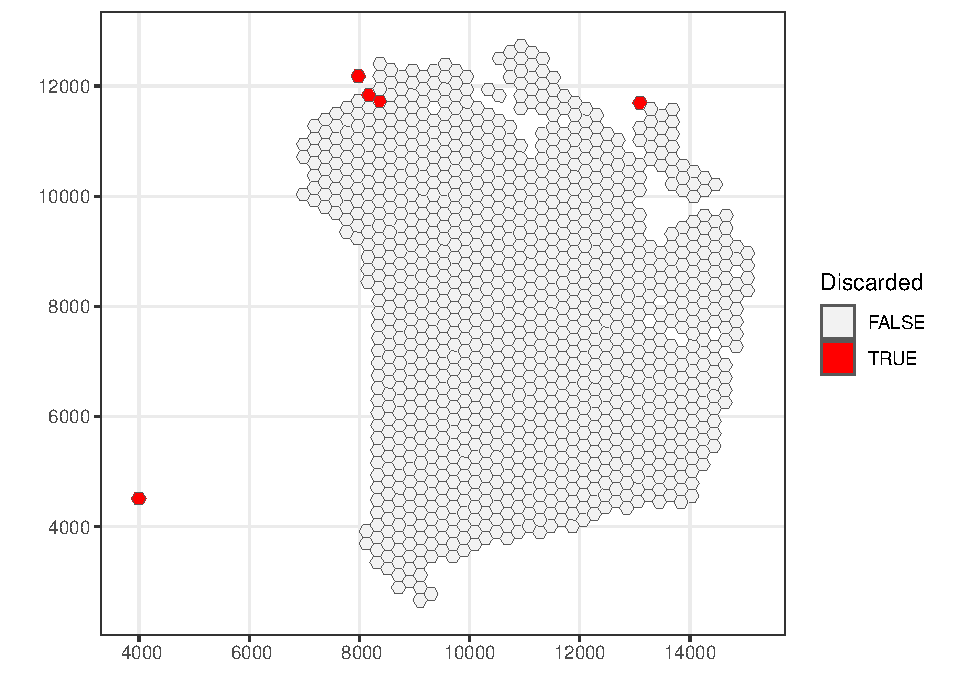
\includegraphics{_main_files/figure-latex/03_QC_sfe5-2.pdf}

\hypertarget{remove-low-quality-spots-1}{%
\subsection{Remove low-quality spots}\label{remove-low-quality-spots-1}}

\begin{Shaded}
\begin{Highlighting}[]
\CommentTok{\# {-}{-}{-}{-}{-}{-}{-}{-}{-}{-}{-}{-}{-}{-}{-}{-}{-}{-}{-}{-}{-}{-}{-}{-}{-}{-}{-}{-}{-}{-}{-}{-}{-}{-}{-}{-}{-}{-}{-}{-}{-}{-}{-}{-}{-}{-}{-} \#}
\DocumentationTok{\#\# Check the number of discarded spots for each metric}
\FunctionTok{apply}\NormalTok{(}\FunctionTok{cbind}\NormalTok{(qc\_lib\_size, qc\_detected, qc\_mito), }\DecValTok{2}\NormalTok{, sum)}
\end{Highlighting}
\end{Shaded}

\begin{verbatim}
## qc_lib_size qc_detected     qc_mito 
##          19          20           5
\end{verbatim}

\begin{Shaded}
\begin{Highlighting}[]
\DocumentationTok{\#\# Combine together the set of discarded spots}
\NormalTok{discard }\OtherTok{\textless{}{-}}\NormalTok{ qc\_lib\_size }\SpecialCharTok{|}\NormalTok{ qc\_detected }\SpecialCharTok{|}\NormalTok{ qc\_mito}
\FunctionTok{table}\NormalTok{(discard)}
\end{Highlighting}
\end{Shaded}

\begin{verbatim}
## discard
## FALSE  TRUE 
##  1161    24
\end{verbatim}

\begin{Shaded}
\begin{Highlighting}[]
\DocumentationTok{\#\# Store the set in the object}
\FunctionTok{colData}\NormalTok{(sfe)}\SpecialCharTok{$}\NormalTok{discard }\OtherTok{\textless{}{-}}\NormalTok{ discard}
\DocumentationTok{\#\# Check for putative spatial pattern of removed spots}
\FunctionTok{ggplot}\NormalTok{() }\SpecialCharTok{+} 
    \FunctionTok{geom\_sf}\NormalTok{(}\AttributeTok{data =} \FunctionTok{colGeometry}\NormalTok{(sfe, }\StringTok{"spotHex"}\NormalTok{),}
            \FunctionTok{aes}\NormalTok{(}\AttributeTok{geometry =}\NormalTok{ geometry)) }\SpecialCharTok{+} 
    \FunctionTok{geom\_sf}\NormalTok{(}\AttributeTok{data =} \FunctionTok{colGeometry}\NormalTok{(sfe, }\StringTok{"spotHex"}\NormalTok{),}
            \FunctionTok{aes}\NormalTok{(}\AttributeTok{geometry =}\NormalTok{ geometry, }\AttributeTok{fill =} \FunctionTok{colData}\NormalTok{(sfe)}\SpecialCharTok{$}\NormalTok{discard)) }\SpecialCharTok{+}
    \FunctionTok{scale\_fill\_manual}\NormalTok{(}\AttributeTok{values =} \FunctionTok{c}\NormalTok{(}\StringTok{"grey95"}\NormalTok{, }\StringTok{"red"}\NormalTok{)) }\SpecialCharTok{+} 
    \FunctionTok{labs}\NormalTok{(}\AttributeTok{fill =} \StringTok{"Discarded"}\NormalTok{) }\SpecialCharTok{+} 
    \FunctionTok{theme\_bw}\NormalTok{()}
\end{Highlighting}
\end{Shaded}

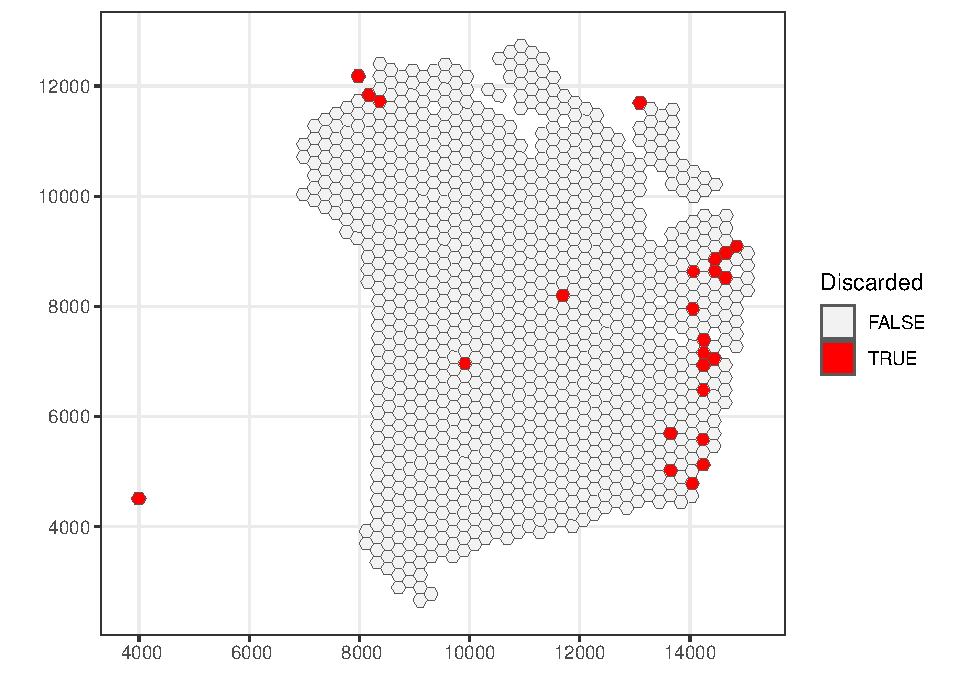
\includegraphics{_main_files/figure-latex/03_QC_sfe6-1.pdf}

\begin{Shaded}
\begin{Highlighting}[]
\CommentTok{\# {-}{-}{-}{-}{-}{-}{-}{-}{-}{-}{-}{-}{-}{-}{-}{-}{-}{-}{-}{-}{-}{-}{-}{-}{-}{-}{-}{-}{-}{-}{-}{-}{-}{-}{-}{-}{-}{-}{-}{-}{-}{-}{-}{-}{-}{-}{-} \#}
\DocumentationTok{\#\# remove combined set of low{-}quality spots}
\NormalTok{sfe }\OtherTok{\textless{}{-}}\NormalTok{ sfe[, }\SpecialCharTok{!}\FunctionTok{colData}\NormalTok{(sfe)}\SpecialCharTok{$}\NormalTok{discard]}
\end{Highlighting}
\end{Shaded}

\hypertarget{normalisation-of-counts-1}{%
\section{Normalisation of counts}\label{normalisation-of-counts-1}}

\hypertarget{log-tranformation-of-counts-1}{%
\subsection{Log-tranformation of counts}\label{log-tranformation-of-counts-1}}

\begin{Shaded}
\begin{Highlighting}[]
\DocumentationTok{\#\# Calculate library size factors}
\NormalTok{sfe }\OtherTok{\textless{}{-}} \FunctionTok{computeLibraryFactors}\NormalTok{(sfe)}
\DocumentationTok{\#\# Have a look at the size factors}
\FunctionTok{summary}\NormalTok{(}\FunctionTok{sizeFactors}\NormalTok{(sfe))}
\end{Highlighting}
\end{Shaded}

\begin{verbatim}
##    Min. 1st Qu.  Median    Mean 3rd Qu.    Max. 
## 0.07961 0.36902 0.95469 1.00000 1.54936 2.77256
\end{verbatim}

\begin{Shaded}
\begin{Highlighting}[]
\DocumentationTok{\#\# Density and histogram of library sizes}
\FunctionTok{ggplot}\NormalTok{(}\AttributeTok{data =} \FunctionTok{data.frame}\NormalTok{(}\AttributeTok{sFact =} \FunctionTok{sizeFactors}\NormalTok{(sfe)), }
       \FunctionTok{aes}\NormalTok{(}\AttributeTok{x =}\NormalTok{ sFact)) }\SpecialCharTok{+}
    \FunctionTok{geom\_histogram}\NormalTok{(}\FunctionTok{aes}\NormalTok{(}\AttributeTok{y =} \FunctionTok{after\_stat}\NormalTok{(density)), }
                   \AttributeTok{colour =} \StringTok{"black"}\NormalTok{, }
                   \AttributeTok{fill =} \StringTok{"grey"}\NormalTok{,}
                   \AttributeTok{bins =} \DecValTok{40}\NormalTok{) }\SpecialCharTok{+}
    \FunctionTok{geom\_density}\NormalTok{(}\AttributeTok{alpha =} \FloatTok{0.5}\NormalTok{,}
                 \AttributeTok{adjust =} \FloatTok{0.5}\NormalTok{,}
                 \AttributeTok{fill =} \StringTok{"\#A0CBE8"}\NormalTok{,}
                 \AttributeTok{colour =} \StringTok{"\#4E79A7"}\NormalTok{) }\SpecialCharTok{+}
    \FunctionTok{scale\_x\_continuous}\NormalTok{(}\AttributeTok{breaks =}\NormalTok{ scales}\SpecialCharTok{::}\FunctionTok{pretty\_breaks}\NormalTok{(}\AttributeTok{n =} \DecValTok{10}\NormalTok{)) }\SpecialCharTok{+} 
    \FunctionTok{scale\_y\_continuous}\NormalTok{(}\AttributeTok{breaks =}\NormalTok{ scales}\SpecialCharTok{::}\FunctionTok{pretty\_breaks}\NormalTok{(}\AttributeTok{n =} \DecValTok{10}\NormalTok{)) }\SpecialCharTok{+} 
    \FunctionTok{xlab}\NormalTok{(}\StringTok{"Library size"}\NormalTok{) }\SpecialCharTok{+} 
    \FunctionTok{ylab}\NormalTok{(}\StringTok{"Density"}\NormalTok{) }\SpecialCharTok{+} 
    \FunctionTok{theme\_classic}\NormalTok{()}
\end{Highlighting}
\end{Shaded}

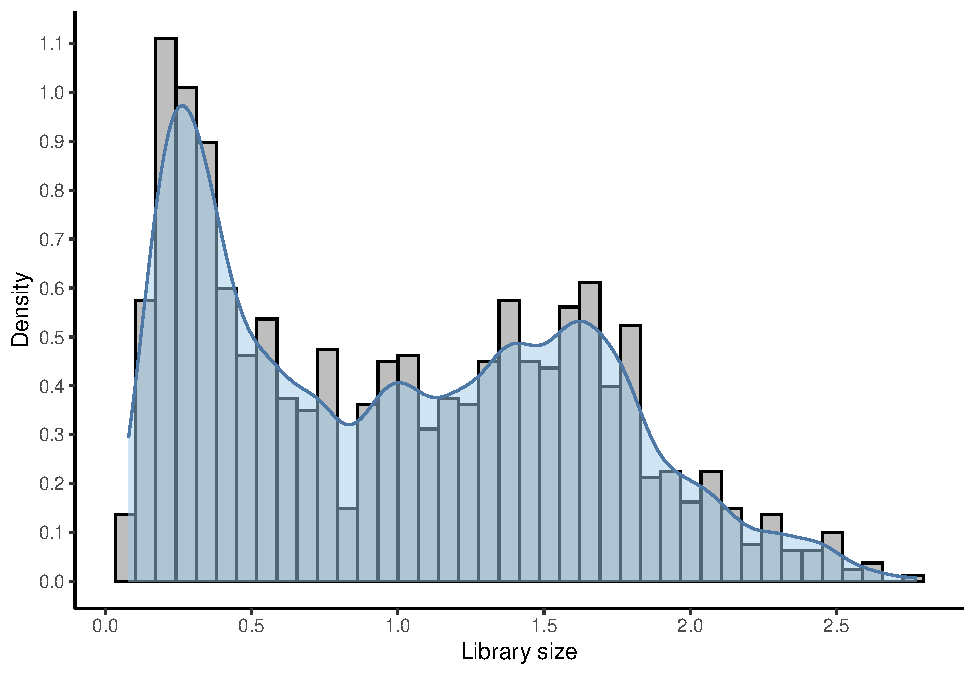
\includegraphics{_main_files/figure-latex/03_LogNorm_sfe-1.pdf}

\begin{Shaded}
\begin{Highlighting}[]
\CommentTok{\# calculate logcounts using library size factors}
\NormalTok{sfe }\OtherTok{\textless{}{-}} \FunctionTok{logNormCounts}\NormalTok{(sfe)}
\end{Highlighting}
\end{Shaded}

\hypertarget{gene-level-quality-control}{%
\section{Gene-level Quality Control}\label{gene-level-quality-control}}

\hypertarget{calculating-extra-qc-metrics}{%
\subsection{Calculating extra QC metrics}\label{calculating-extra-qc-metrics}}

\begin{Shaded}
\begin{Highlighting}[]
\FunctionTok{rowData}\NormalTok{(sfe)[[}\StringTok{"JBO019.s\_logMean"}\NormalTok{]] }\OtherTok{\textless{}{-}} \FunctionTok{rowSums}\NormalTok{(}\FunctionTok{assay}\NormalTok{(sfe, }\StringTok{"logcounts"}\NormalTok{)) }\SpecialCharTok{/} \FunctionTok{rowData}\NormalTok{(sfe)[[}\StringTok{"JBO019.nLocations"}\NormalTok{]]}
\end{Highlighting}
\end{Shaded}

\hypertarget{set-and-apply-filters}{%
\subsection{Set and apply filters}\label{set-and-apply-filters}}

\begin{Shaded}
\begin{Highlighting}[]
\NormalTok{is\_zero }\OtherTok{\textless{}{-}} \FunctionTok{rowData}\NormalTok{(sfe)}\SpecialCharTok{$}\NormalTok{total }\SpecialCharTok{==} \DecValTok{0}
\NormalTok{is\_logLow }\OtherTok{\textless{}{-}} \FunctionTok{rowData}\NormalTok{(sfe)[[}\StringTok{"JBO019.s\_logMean"}\NormalTok{]] }\SpecialCharTok{\textless{}=} \DecValTok{1}
\NormalTok{discard\_gs }\OtherTok{\textless{}{-}}\NormalTok{ is\_zero }\SpecialCharTok{|}\NormalTok{ is\_mito }\SpecialCharTok{|}\NormalTok{ is\_logLow}
\FunctionTok{table}\NormalTok{(discard\_gs)}
\end{Highlighting}
\end{Shaded}

\begin{verbatim}
## discard_gs
## FALSE  TRUE 
##  8535 24203
\end{verbatim}

\begin{Shaded}
\begin{Highlighting}[]
\FunctionTok{rowData}\NormalTok{(sfe)}\SpecialCharTok{$}\NormalTok{discard }\OtherTok{\textless{}{-}}\NormalTok{ discard\_gs}

\DocumentationTok{\#\# FEATURE SELECTION}
\DocumentationTok{\#\# remove mitochondrial and other genes}
\NormalTok{sfe }\OtherTok{\textless{}{-}}\NormalTok{ sfe[}\SpecialCharTok{!}\FunctionTok{rowData}\NormalTok{(sfe)}\SpecialCharTok{$}\NormalTok{discard, ]}
\end{Highlighting}
\end{Shaded}

\hypertarget{selecting-genes-1}{%
\section{Selecting genes}\label{selecting-genes-1}}

\hypertarget{highly-variable-genes-hvgs-1}{%
\subsection{Highly Variable Genes (HVGs)}\label{highly-variable-genes-hvgs-1}}

\begin{Shaded}
\begin{Highlighting}[]
\DocumentationTok{\#\# Fit mean{-}variance relationship}
\NormalTok{dec }\OtherTok{\textless{}{-}} \FunctionTok{modelGeneVar}\NormalTok{(sfe,}
                    \AttributeTok{assay.type =} \StringTok{"logcounts"}\NormalTok{)}

\DocumentationTok{\#\# Visualize mean{-}variance relationship}
\NormalTok{fit }\OtherTok{\textless{}{-}} \FunctionTok{metadata}\NormalTok{(dec)}
\NormalTok{fit\_df }\OtherTok{\textless{}{-}} \FunctionTok{data.frame}\NormalTok{(}\AttributeTok{mean =}\NormalTok{ fit}\SpecialCharTok{$}\NormalTok{mean,}
                     \AttributeTok{var =}\NormalTok{ fit}\SpecialCharTok{$}\NormalTok{var,}
                     \AttributeTok{trend =}\NormalTok{ fit}\SpecialCharTok{$}\FunctionTok{trend}\NormalTok{(fit}\SpecialCharTok{$}\NormalTok{mean))}

\FunctionTok{ggplot}\NormalTok{(}\AttributeTok{data =}\NormalTok{ fit\_df, }
       \FunctionTok{aes}\NormalTok{(}\AttributeTok{x =}\NormalTok{ mean, }\AttributeTok{y =}\NormalTok{ var)) }\SpecialCharTok{+} 
    \FunctionTok{geom\_point}\NormalTok{() }\SpecialCharTok{+} 
    \FunctionTok{geom\_line}\NormalTok{(}\FunctionTok{aes}\NormalTok{(}\AttributeTok{y =}\NormalTok{ trend), }\AttributeTok{colour =} \StringTok{"dodgerblue"}\NormalTok{, }\AttributeTok{linewidth =} \FloatTok{1.5}\NormalTok{) }\SpecialCharTok{+} 
    \FunctionTok{labs}\NormalTok{(}\AttributeTok{x =} \StringTok{"mean of log{-}expression"}\NormalTok{,}
         \AttributeTok{y =} \StringTok{"variance of log{-}expression"}\NormalTok{) }\SpecialCharTok{+} 
    \FunctionTok{theme\_classic}\NormalTok{()}
\end{Highlighting}
\end{Shaded}

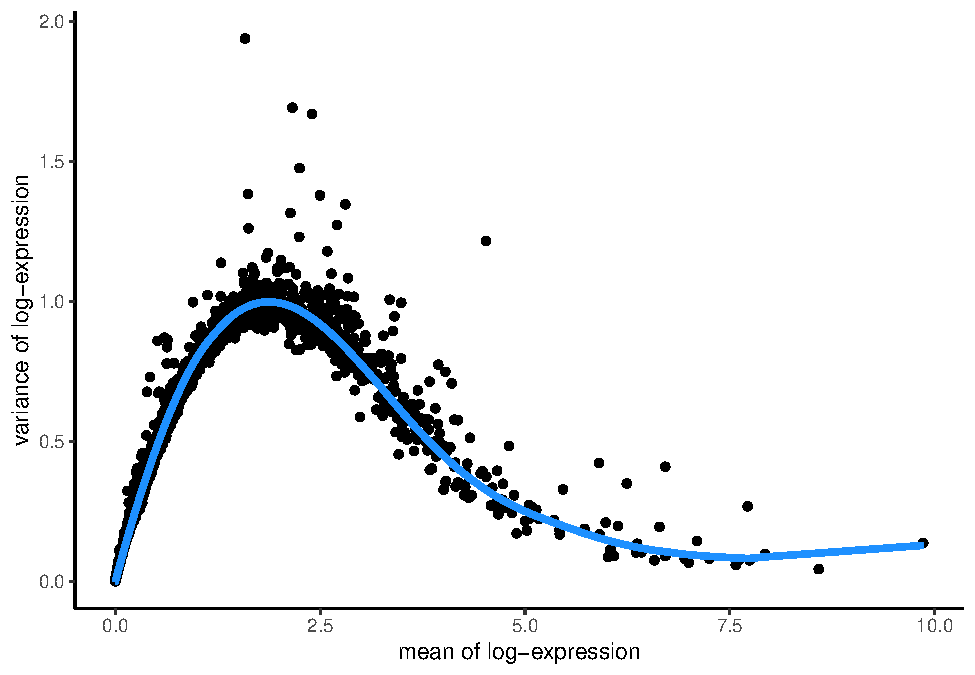
\includegraphics{_main_files/figure-latex/03_HVGs_sfe-1.pdf}

\begin{Shaded}
\begin{Highlighting}[]
\DocumentationTok{\#\# Select top HVGs}
\NormalTok{top\_hvgs }\OtherTok{\textless{}{-}} \FunctionTok{getTopHVGs}\NormalTok{(dec, }
                       \AttributeTok{var.field =} \StringTok{"bio"}\NormalTok{, }
                       \AttributeTok{prop =} \FloatTok{0.5}\NormalTok{,}
                       \AttributeTok{var.threshold =} \DecValTok{0}\NormalTok{,}
                       \AttributeTok{fdr.threshold =} \FloatTok{0.1}\NormalTok{)}
\end{Highlighting}
\end{Shaded}

\hypertarget{neighbour-graph-and-distance-matrix}{%
\section{Neighbour graph and distance matrix}\label{neighbour-graph-and-distance-matrix}}

\hypertarget{adding-spatial-weights}{%
\subsection{Adding spatial weights}\label{adding-spatial-weights}}

The neighbour lists can be supplemented with spatial weights using the \texttt{nb2listw} and \texttt{nb2listwdist} function from \texttt{spdep} package for the chosen type and coding scheme style. There are 6 different coding scheme styles that can be used to weigh neighbour relationships:

\begin{enumerate}
\def\labelenumi{\arabic{enumi}.}
\tightlist
\item
  \textbf{B}: is the basic binary coding (1 for neighbour, 0 for no neighbour).
\item
  \textbf{W}: is row standardised (sums over all links to n).
\item
  \textbf{C}: is globally standardised (sums over all links to n).
\item
  \textbf{U}: is equal to C divided by the number of neighbours (sums over all links to unity).
\item
  \textbf{S}: is the variance-stabilizing coding scheme (sums over all links to n).
\item
  \textbf{minmax}: divides the weights by the minimum of the maximum row sums and maximum column sums of the input weights; It is similar to the C and U styles.
\end{enumerate}

The coding scheme style is practically the value each neighbour will get. For example, in a binary coding scheme style (\textbf{B}) if a spot is a neighbour of the spot in focus then gets the value of \textbf{1}, else gets \textbf{0}. Another example, in a row standardised coding scheme style (\textbf{W}) if the spot in focus has a total of 10 neighbours and each neighbour has a weight of 1, then the sum of all neighbour weights is 10, and each neighbour will get a normalised weight of 1/10 = 0.1. As a result, in the row standardised coding scheme, spots with many neighbours will have neighbours with lower weights and thus will not be over-emphasised.

Starting from a binary neighbours list, in which regions are either listed as neighbours or are absent (thus not in the set of neighbours for some definition), we can add a distance-based weights list. The \texttt{nb2listwdist} function supplements a neighbours list with spatial weights for the chosen types of distance modelling and coding scheme. While the offered coding schemes parallel those of the \texttt{nb2listw} function above, three distance-based types of weights are available: inverse distance weighting (IDW), double-power distance weights (DPD), and exponential distance decay (EXP). The three types of distance weight calculations are based on pairwise distances 𝑑𝑖𝑗, all of which are controlled by parameter \emph{``alpha''} (𝛼 below):

\begin{enumerate}
\def\labelenumi{\arabic{enumi}.}
\tightlist
\item
  \textbf{idw}: 𝑤𝑖𝑗=𝑑−𝛼𝑖𝑗,
\item
  \textbf{exp}: 𝑤𝑖𝑗=exp(−𝛼⋅𝑑𝑖𝑗),
\item
  \textbf{dpd}: 𝑤𝑖𝑗={[}1−(𝑑𝑖𝑗/𝑑max)𝛼{]}𝛼,
\end{enumerate}

the latter of which leads to 𝑤𝑖𝑗=0 for all 𝑑𝑖𝑗\textgreater 𝑑max. Note that \emph{IDW} weights show extreme behaviour close to 0 and can take on the value infinity. In such cases, the infinite values are replaced by the largest finite weight present in the weights list.

\hypertarget{generate-distance-matrices}{%
\subsection{Generate distance matrices}\label{generate-distance-matrices}}

A distance matrix is a mirrored matrix that contains the distance between a spot and every other spot. This distance can be a simple Euclidean distance based on the coordinates of the spots or a weighted distance according to a bandwidth around each spot using a kernel that gives higher scores to distances between spots that are closer together compared to the ones that are farther away. These weighted distance matrices are later used to run geographically weighted (GW) models.

There are 6 different kernels that can be used to weight the distances between spots. The next two figures are from the \texttt{GWmodel}'s publication \citep{Gollini2015Feb} and provide a bit more description on that.

\begin{figure}

{\centering 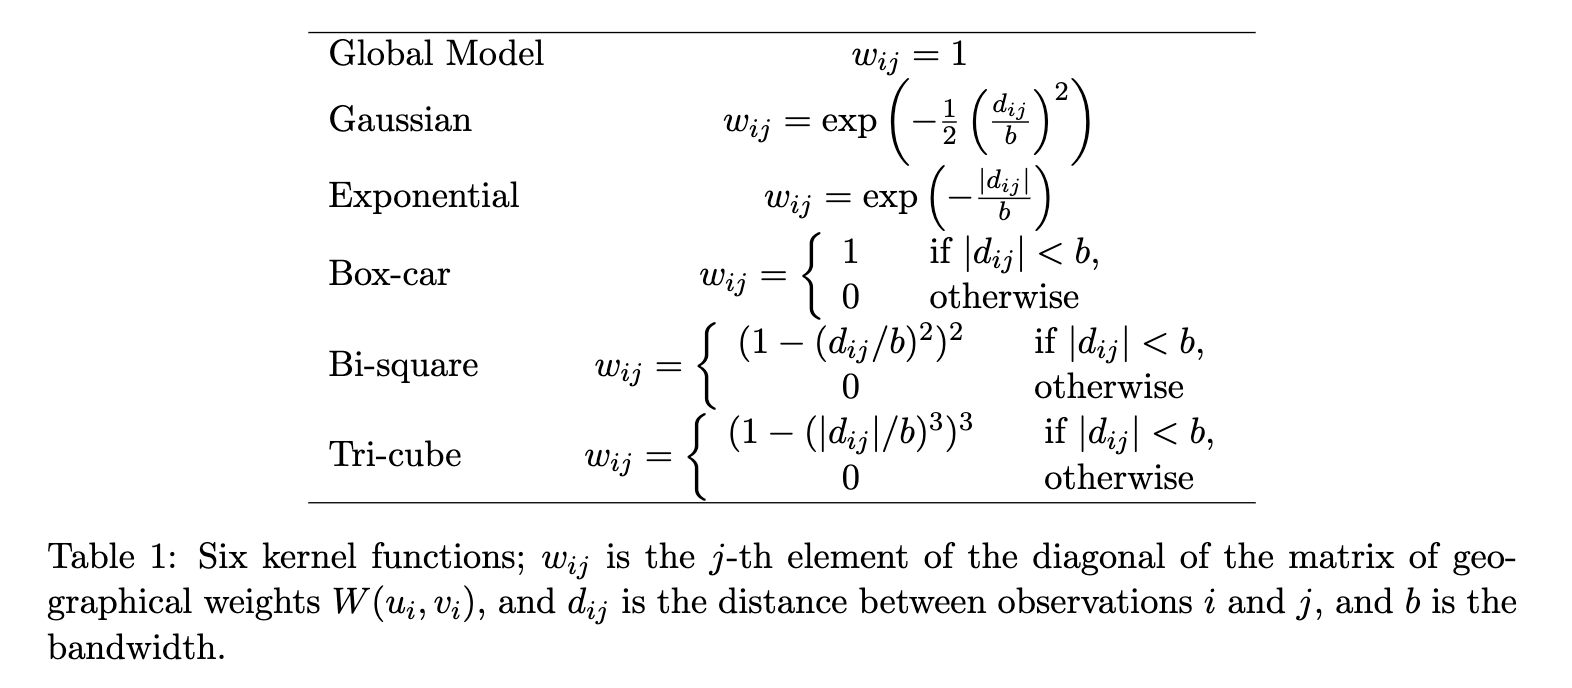
\includegraphics[width=1\linewidth]{images/gwmodel_kernel_math} 

}

\caption{The math equations that define the kernels.}\label{fig:GWmodelFig1}
\end{figure}

\begin{figure}

{\centering 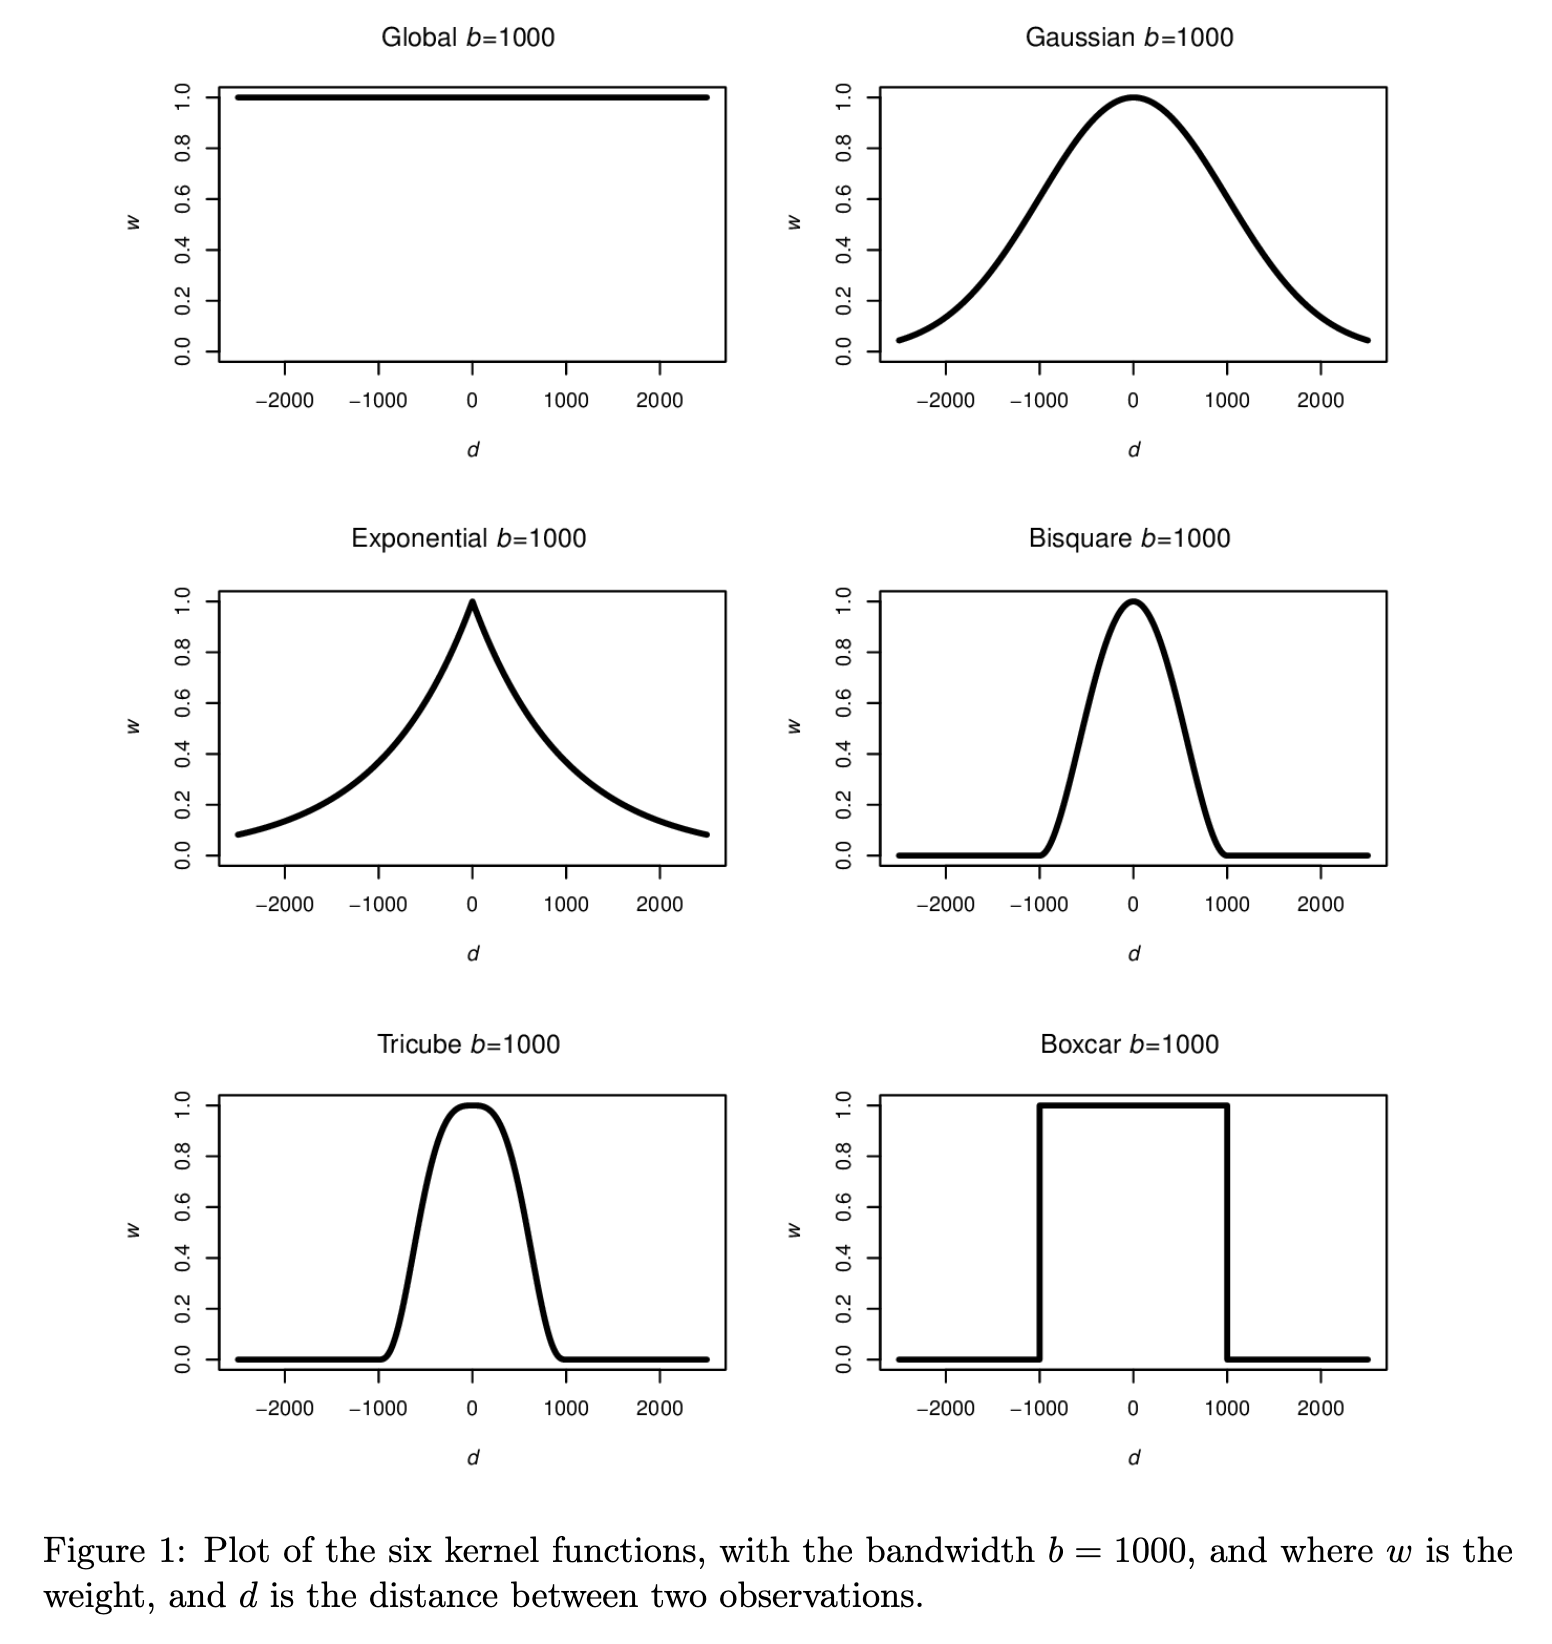
\includegraphics[width=1\linewidth]{images/gwmodel_kernel_graphs} 

}

\caption{Examples from using each kernel.}\label{fig:GWmodelFig2}
\end{figure}

\begin{Shaded}
\begin{Highlighting}[]
\DocumentationTok{\#\# add a neighbour graph using a weighted distance matrix}
\NormalTok{sfe }\OtherTok{\textless{}{-}} \FunctionTok{addSpatialNeighGraphs}\NormalTok{(sfe, }\StringTok{"JBO019"}\NormalTok{, }\AttributeTok{type =} \StringTok{"knearneigh"}\NormalTok{, }\AttributeTok{style =} \StringTok{"W"}\NormalTok{, }\AttributeTok{distMod =} \StringTok{"raw"}\NormalTok{, }\AttributeTok{k =} \DecValTok{6}\NormalTok{)}

\FunctionTok{colGraphs}\NormalTok{(sfe)}
\end{Highlighting}
\end{Shaded}

\begin{verbatim}
## $col
## Characteristics of weights list object:
## Neighbour list object:
## Number of regions: 1161 
## Number of nonzero links: 6966 
## Percentage nonzero weights: 0.5167959 
## Average number of links: 6 
## Non-symmetric neighbours list
## 
## Weights style: W 
## Weights constants summary:
##      n      nn   S0       S1       S2
## W 1161 1347921 1161 376.8333 4674.667
\end{verbatim}

\begin{Shaded}
\begin{Highlighting}[]
\DocumentationTok{\#\# Calculate a simple distance matrix}
\NormalTok{sfe }\OtherTok{\textless{}{-}} \FunctionTok{addDistMat}\NormalTok{(sfe, }\AttributeTok{p =} \DecValTok{2}\NormalTok{)}
\end{Highlighting}
\end{Shaded}

\hypertarget{putting-it-all-together-1}{%
\section{Putting it all together}\label{putting-it-all-together-1}}

The below code puts all these steps in order by selecting one of the options at each step.

\begin{Shaded}
\begin{Highlighting}[]
\DocumentationTok{\#\# Import data}
\NormalTok{sampleDir }\OtherTok{\textless{}{-}} \StringTok{"./data/spaceranger\_outs/Human\_Liver\_Steatotic/JBO019\_Results"}
\NormalTok{sampleNames }\OtherTok{\textless{}{-}} \StringTok{"JBO019"}
\NormalTok{sfe }\OtherTok{\textless{}{-}} \FunctionTok{read10xVisiumSFE}\NormalTok{(}\AttributeTok{samples =}\NormalTok{ sampleDir, }
                        \AttributeTok{sample\_id =}\NormalTok{ sampleNames, }
                        \AttributeTok{type =} \StringTok{"sparse"}\NormalTok{, }
                        \AttributeTok{data =} \StringTok{"filtered"}\NormalTok{, }
                        \AttributeTok{images =} \StringTok{"lowres"}\NormalTok{, }
                        \AttributeTok{style =} \StringTok{"W"}\NormalTok{, }
                        \AttributeTok{zero.policy =} \ConstantTok{TRUE}\NormalTok{)}
\CommentTok{\# {-}{-}{-}{-}{-}{-}{-}{-}{-}{-}{-}{-}{-}{-}{-}{-}{-}{-}{-}{-}{-}{-}{-}{-}{-}{-}{-}{-}{-}{-}{-}{-}{-}{-}{-}{-}{-}{-}{-}{-}{-}{-}{-}{-}{-}{-}{-} \#}
\NormalTok{ground\_truth }\OtherTok{\textless{}{-}} \FunctionTok{read\_table}\NormalTok{(}\StringTok{"./data/to\_load/spotzonationGroup.txt"}\NormalTok{)}
\DocumentationTok{\#\# Add QC metrics}
\NormalTok{is\_mito }\OtherTok{\textless{}{-}} \FunctionTok{grepl}\NormalTok{(}\StringTok{"(\^{}MT{-})|(\^{}mt{-})"}\NormalTok{, }\FunctionTok{rowData}\NormalTok{(sfe)}\SpecialCharTok{$}\NormalTok{symbol)}
\NormalTok{sfe }\OtherTok{\textless{}{-}} \FunctionTok{addPerLocQC}\NormalTok{(sfe, }\AttributeTok{gTruth =}\NormalTok{ ground\_truth, }\AttributeTok{assay =} \StringTok{"counts"}\NormalTok{, }\DecValTok{2}\NormalTok{, }\AttributeTok{subsets =} \FunctionTok{list}\NormalTok{(}\AttributeTok{mito =}\NormalTok{ is\_mito))}
\NormalTok{sfe }\OtherTok{\textless{}{-}} \FunctionTok{addGeometries}\NormalTok{(sfe, }\AttributeTok{samples =}\NormalTok{ sampleDir, }\AttributeTok{sample\_id =}\NormalTok{ sampleNames, }\AttributeTok{res =} \StringTok{"fullres"}\NormalTok{)}
\NormalTok{sfe }\OtherTok{\textless{}{-}} \FunctionTok{addPerGeneQC}\NormalTok{(sfe, }\AttributeTok{assay =} \StringTok{"counts"}\NormalTok{, }\AttributeTok{version =} \ConstantTok{NULL}\NormalTok{, }\AttributeTok{mirror =} \ConstantTok{NULL}\NormalTok{)}
\CommentTok{\# {-}{-}{-}{-}{-}{-}{-}{-}{-}{-}{-}{-}{-}{-}{-}{-}{-}{-}{-}{-}{-}{-}{-}{-}{-}{-}{-}{-}{-}{-}{-}{-}{-}{-}{-}{-}{-}{-}{-}{-}{-}{-}{-}{-}{-}{-}{-} \#}
\DocumentationTok{\#\# SPOT SELECTION}
\DocumentationTok{\#\# Select library size threshold}
\NormalTok{qc\_lib\_size }\OtherTok{\textless{}{-}} \FunctionTok{colData}\NormalTok{(sfe)}\SpecialCharTok{$}\NormalTok{sum }\SpecialCharTok{\textless{}} \DecValTok{1000}
\DocumentationTok{\#\# Add threshold in colData}
\FunctionTok{colData}\NormalTok{(sfe)}\SpecialCharTok{$}\NormalTok{qc\_lib\_size }\OtherTok{\textless{}{-}}\NormalTok{ qc\_lib\_size}
\DocumentationTok{\#\# Select expressed genes threshold}
\NormalTok{qc\_detected }\OtherTok{\textless{}{-}} \FunctionTok{colData}\NormalTok{(sfe)}\SpecialCharTok{$}\NormalTok{detected }\SpecialCharTok{\textless{}} \DecValTok{550}
\DocumentationTok{\#\# Add threshold in colData}
\FunctionTok{colData}\NormalTok{(sfe)}\SpecialCharTok{$}\NormalTok{qc\_detected }\OtherTok{\textless{}{-}}\NormalTok{ qc\_detected}
\DocumentationTok{\#\# Select mitochondrial percentage threshold}
\NormalTok{qc\_mito }\OtherTok{\textless{}{-}} \FunctionTok{colData}\NormalTok{(sfe)}\SpecialCharTok{$}\NormalTok{subsets\_mito\_percent }\SpecialCharTok{\textgreater{}} \DecValTok{22}
\DocumentationTok{\#\# Add threshold in colData}
\FunctionTok{colData}\NormalTok{(sfe)}\SpecialCharTok{$}\NormalTok{qc\_mito }\OtherTok{\textless{}{-}}\NormalTok{ qc\_mito}
\DocumentationTok{\#\# Combine together the set of discarded spots}
\NormalTok{discard }\OtherTok{\textless{}{-}}\NormalTok{ qc\_lib\_size }\SpecialCharTok{|}\NormalTok{ qc\_detected }\SpecialCharTok{|}\NormalTok{ qc\_mito}
\DocumentationTok{\#\# Store the set in the object}
\FunctionTok{colData}\NormalTok{(sfe)}\SpecialCharTok{$}\NormalTok{discard }\OtherTok{\textless{}{-}}\NormalTok{ discard}
\DocumentationTok{\#\# Remove combined set of low{-}quality spots}
\NormalTok{sfe }\OtherTok{\textless{}{-}}\NormalTok{ sfe[, }\SpecialCharTok{!}\FunctionTok{colData}\NormalTok{(sfe)}\SpecialCharTok{$}\NormalTok{discard]}
\CommentTok{\# {-}{-}{-}{-}{-}{-}{-}{-}{-}{-}{-}{-}{-}{-}{-}{-}{-}{-}{-}{-}{-}{-}{-}{-}{-}{-}{-}{-}{-}{-}{-}{-}{-}{-}{-}{-}{-}{-}{-}{-}{-}{-}{-}{-}{-}{-}{-} \#}
\DocumentationTok{\#\# FEATURE SELECTION}
\DocumentationTok{\#\# Calculate library size factors}
\NormalTok{sfe }\OtherTok{\textless{}{-}} \FunctionTok{computeLibraryFactors}\NormalTok{(sfe)}
\DocumentationTok{\#\# Calculate logcounts using library size factors}
\NormalTok{sfe }\OtherTok{\textless{}{-}} \FunctionTok{logNormCounts}\NormalTok{(sfe)}
\DocumentationTok{\#\# Calculate log{-}counts sample mean}
\FunctionTok{rowData}\NormalTok{(sfe)[[}\StringTok{"JBO019.s\_logMean"}\NormalTok{]] }\OtherTok{\textless{}{-}} \FunctionTok{rowSums}\NormalTok{(}\FunctionTok{assay}\NormalTok{(sfe, }\StringTok{"logcounts"}\NormalTok{)) }\SpecialCharTok{/} \FunctionTok{rowData}\NormalTok{(sfe)[[}\StringTok{"JBO019.nLocations"}\NormalTok{]]}
\DocumentationTok{\#\# Set and apply filters}
\NormalTok{is\_zero }\OtherTok{\textless{}{-}} \FunctionTok{rowData}\NormalTok{(sfe)}\SpecialCharTok{$}\NormalTok{total }\SpecialCharTok{==} \DecValTok{0}
\NormalTok{is\_logLow }\OtherTok{\textless{}{-}} \FunctionTok{rowData}\NormalTok{(sfe)[[}\StringTok{"JBO019.s\_logMean"}\NormalTok{]] }\SpecialCharTok{\textless{}=} \DecValTok{1}
\NormalTok{discard\_gs }\OtherTok{\textless{}{-}}\NormalTok{ is\_zero }\SpecialCharTok{|}\NormalTok{ is\_mito }\SpecialCharTok{|}\NormalTok{ is\_logLow}
\FunctionTok{rowData}\NormalTok{(sfe)}\SpecialCharTok{$}\NormalTok{discard }\OtherTok{\textless{}{-}}\NormalTok{ discard\_gs}
\DocumentationTok{\#\# Remove mitochondrial and other genes}
\NormalTok{sfe }\OtherTok{\textless{}{-}}\NormalTok{ sfe[}\SpecialCharTok{!}\FunctionTok{rowData}\NormalTok{(sfe)}\SpecialCharTok{$}\NormalTok{discard, ]}
\DocumentationTok{\#\# Fit mean{-}variance relationship}
\NormalTok{dec }\OtherTok{\textless{}{-}} \FunctionTok{modelGeneVar}\NormalTok{(sfe,}
                    \AttributeTok{assay.type =} \StringTok{"logcounts"}\NormalTok{)}
\DocumentationTok{\#\# Select top HVGs}
\NormalTok{top\_hvgs }\OtherTok{\textless{}{-}} \FunctionTok{getTopHVGs}\NormalTok{(dec, }
                       \AttributeTok{var.field =} \StringTok{"bio"}\NormalTok{, }
                       \AttributeTok{prop =} \FloatTok{0.5}\NormalTok{,}
                       \AttributeTok{var.threshold =} \DecValTok{0}\NormalTok{,}
                       \AttributeTok{fdr.threshold =} \FloatTok{0.05}\NormalTok{)}
\CommentTok{\# {-}{-}{-}{-}{-}{-}{-}{-}{-}{-}{-}{-}{-}{-}{-}{-}{-}{-}{-}{-}{-}{-}{-}{-}{-}{-}{-}{-}{-}{-}{-}{-}{-}{-}{-}{-}{-}{-}{-}{-}{-}{-}{-}{-}{-}{-}{-} \#}
\DocumentationTok{\#\# ADD GEOGRAPHY}
\DocumentationTok{\#\# Add a neighbour graph using a weighted distance matrix}
\NormalTok{sfe }\OtherTok{\textless{}{-}} \FunctionTok{addSpatialNeighGraphs}\NormalTok{(sfe, }\StringTok{"JBO019"}\NormalTok{, }\AttributeTok{type =} \StringTok{"knearneigh"}\NormalTok{, }\AttributeTok{style =} \StringTok{"W"}\NormalTok{, }\AttributeTok{distMod =} \StringTok{"raw"}\NormalTok{, }\AttributeTok{k =} \DecValTok{6}\NormalTok{)}
\DocumentationTok{\#\# Calculate a simple distance matrix}
\NormalTok{sfe }\OtherTok{\textless{}{-}} \FunctionTok{addDistMat}\NormalTok{(sfe, }\AttributeTok{p =} \DecValTok{2}\NormalTok{)}
\end{Highlighting}
\end{Shaded}

\hypertarget{save-data}{%
\section{Save data}\label{save-data}}

\hypertarget{practical-session-4}{%
\chapter{Practical session 4}\label{practical-session-4}}

In this session we will have a hands-on exploration of GW-PCA and its application to STx data. What can we learn from this novel technique?

\hypertarget{geographically-weighted-principal-components-analysis-gwpca}{%
\section{Geographically Weighted Principal Components Analysis (GWPCA)}\label{geographically-weighted-principal-components-analysis-gwpca}}

A standard PCA can pick out the key multivariate modes of variability in the data. Looking at outlying values of the principal components of these data gives us an idea of unusual sites (in terms of combinations of gene expression profiles -and to a certain extend of combinations of cell types in each spot). Next, Geographically weighted PCA can be used to find spatial multivariate outliers. Sounds complicated, but really all this means is it identifies sites that have an unusual multi-way combination of gene expression in relation to their immediate geographical neighbours. It might be that the values observed at these sites as a combination is not uncommon in the tissue as a whole - but is very unusual in its locality.

To find such outliers the procedure is relatively simple - instead of doing a PCA on the tissue as a whole, for each sample we do a PCA on data falling into a window centred on the location of that spot. In that way we can check whether the spot is like its neighbours or not, from a multivariate viewpoint.

The following code carries out a geographically weighted PCA. In short, it runs a `windowed' PCA around each of the spots.

\hypertarget{load-packages}{%
\section{Load packages}\label{load-packages}}

\hypertarget{load-quality-controled-and-normalised-data}{%
\section{Load Quality Controled and Normalised data}\label{load-quality-controled-and-normalised-data}}

\begin{Shaded}
\begin{Highlighting}[]
\NormalTok{sfe }\OtherTok{\textless{}{-}} \FunctionTok{readRDS}\NormalTok{(}\AttributeTok{file =} \StringTok{"./data/to\_load/practical03\_sfe.rds"}\NormalTok{)}
\NormalTok{top\_hvgs }\OtherTok{\textless{}{-}} \FunctionTok{readRDS}\NormalTok{(}\AttributeTok{file =} \StringTok{"./data/to\_load/practical03\_topHVGs.rds"}\NormalTok{)}
\end{Highlighting}
\end{Shaded}

\hypertarget{parameter-prearation-for-gwpca}{%
\section{Parameter prearation for GWPCA}\label{parameter-prearation-for-gwpca}}

Because gwpca uses princomp to run the PCAs and this does not accept the number of variables (genes) being more than the number of samples (spots).

\begin{Shaded}
\begin{Highlighting}[]
\DocumentationTok{\#\# Get the gene names that are going to be evaluated}
\NormalTok{vars }\OtherTok{=}\NormalTok{ top\_hvgs}
\DocumentationTok{\#\# Set a fixed bandwidth}
\NormalTok{bw }\OtherTok{=} \DecValTok{6}\SpecialCharTok{*}\NormalTok{sfe}\SpecialCharTok{@}\NormalTok{metadata[[}\StringTok{"spotDiameter"}\NormalTok{]][[}\StringTok{"JBO019"}\NormalTok{]][[}\StringTok{"spot\_diameter\_fullres"}\NormalTok{]]}
\DocumentationTok{\#\# Set the number of components to be retained}
\NormalTok{k }\OtherTok{=} \DecValTok{20}
\DocumentationTok{\#\# Set the kernel to be used}
\NormalTok{kernel }\OtherTok{=} \StringTok{"gaussian"}
\DocumentationTok{\#\# Set the Minkowski distance power: p = 2 {-}{-}\textgreater{} Euclidean}
\NormalTok{p }\OtherTok{=} \DecValTok{2}
\DocumentationTok{\#\# Is the bandwidth adaptive?: No because spots are fixed}
\NormalTok{adaptive }\OtherTok{=} \ConstantTok{FALSE}
\DocumentationTok{\#\# Cross{-}Validate GWPCA?}
\NormalTok{cv }\OtherTok{=} \ConstantTok{TRUE}
\DocumentationTok{\#\# Calculate PCA scores?}
\NormalTok{scores }\OtherTok{=} \ConstantTok{FALSE}
\DocumentationTok{\#\# Run a robust GWPCA?}
\NormalTok{robust }\OtherTok{=} \ConstantTok{FALSE}
\DocumentationTok{\#\# Make a cluster for parallel computing (otherwise GWPCA is slow!)}
\NormalTok{my.cl }\OtherTok{\textless{}{-}}\NormalTok{ parallel}\SpecialCharTok{::}\FunctionTok{makeCluster}\NormalTok{(parallelly}\SpecialCharTok{::}\FunctionTok{availableCores}\NormalTok{() }\SpecialCharTok{{-}} \DecValTok{1}\NormalTok{, }\AttributeTok{type =} \StringTok{\textquotesingle{}FORK\textquotesingle{}}\NormalTok{)}
\end{Highlighting}
\end{Shaded}

The bandwidth is essentially the radius around each spot where every other spot that falls inside it is considered a neighbour. We can set bandwidth as a fixed value or we can select the bandwidth automatically. Without going into detail here, this is achieved by a form of cross validation, where each observation is omitted, and it is attempted to reconstruct the values on the basis of principal components, derived from the other observations. The bandwidth achieving the optimal results is the one selected. For a complete explanation, see \citet{Harris2011Oct}. The function \texttt{bw.gwpca} computes this:

\begin{itemize}
\tightlist
\item
  \textbf{NOTE}: Larger bandwidths imply bigger moving spatial windows, which in turn imply smoother spatially varying outputs.
\end{itemize}

\hypertarget{run-gwpca}{%
\section{Run GWPCA}\label{run-gwpca}}

Run the optimised GWPCA with the automatically estimated bandwidth:

\begin{Shaded}
\begin{Highlighting}[]
\CommentTok{\# DO NOT RUN THIS CHUNK}
\CommentTok{\# \textgreater{}\textgreater{}\textgreater{} it returns an error when inside the markdown. Maybe run with verbose = FALSE}
\NormalTok{pcagw }\OtherTok{\textless{}{-}} \FunctionTok{gwpcaSTE}\NormalTok{(}\AttributeTok{sfe =}\NormalTok{ sfe, }
                  \AttributeTok{assay =} \StringTok{"logcounts"}\NormalTok{,}
                  \AttributeTok{vars =}\NormalTok{ vars, }
                  \AttributeTok{p =}\NormalTok{ p, }
                  \AttributeTok{k =}\NormalTok{ k, }
                  \AttributeTok{bw =}\NormalTok{ bw, }
                  \AttributeTok{kernel =}\NormalTok{ kernel,}
                  \AttributeTok{adaptive =}\NormalTok{ adaptive, }
                  \AttributeTok{scores =}\NormalTok{ scores, }
                  \AttributeTok{robust =}\NormalTok{ robust,}
                  \AttributeTok{cv =}\NormalTok{ cv,}
                  \AttributeTok{future =} \ConstantTok{FALSE}\NormalTok{,}
                  \AttributeTok{strategy =} \StringTok{"cluster"}\NormalTok{,}
                  \AttributeTok{workers =}\NormalTok{ my.cl,}
                  \AttributeTok{verbose =} \ConstantTok{FALSE}\NormalTok{)}
\FunctionTok{saveRDS}\NormalTok{(pcagw, }\AttributeTok{file =} \StringTok{"./data/to\_load/practical04\_pcagw.rds"}\NormalTok{)}
\end{Highlighting}
\end{Shaded}

Because GWPCA can take some time to run, we ran it for you and below you can load the output:

\begin{Shaded}
\begin{Highlighting}[]
\NormalTok{pcagw }\OtherTok{\textless{}{-}} \FunctionTok{readRDS}\NormalTok{(}\AttributeTok{file =} \StringTok{"./data/to\_load/practical04\_pcagw.rds"}\NormalTok{)}
\end{Highlighting}
\end{Shaded}

\hypertarget{plot-global-pca-results}{%
\section{Plot global PCA results}\label{plot-global-pca-results}}

In the next steps we will be looking inside the output from \texttt{gwpca} function and we are going to extract some basic information. Since GWPCA is multiple local PCAs, it is good to know how many PCs makes sense to look at. We can do so by running a global PCA and plotting a scree plot:

\begin{Shaded}
\begin{Highlighting}[]
\FunctionTok{plotGWPCA\_global}\NormalTok{(}\AttributeTok{gwpca =}\NormalTok{ pcagw,}
                 \AttributeTok{comps =} \DecValTok{1}\SpecialCharTok{:}\DecValTok{10}\NormalTok{,}
                 \AttributeTok{type =} \StringTok{"scree"}\NormalTok{,}
                 \AttributeTok{point\_args =} \FunctionTok{list}\NormalTok{(}\AttributeTok{size =} \DecValTok{3}\NormalTok{, }\AttributeTok{colour =} \StringTok{"red"}\NormalTok{),}
                 \AttributeTok{line\_args =} \FunctionTok{list}\NormalTok{(}\AttributeTok{linewidth =} \DecValTok{1}\NormalTok{, }\AttributeTok{colour =} \StringTok{"dodgerblue"}\NormalTok{))}
\end{Highlighting}
\end{Shaded}

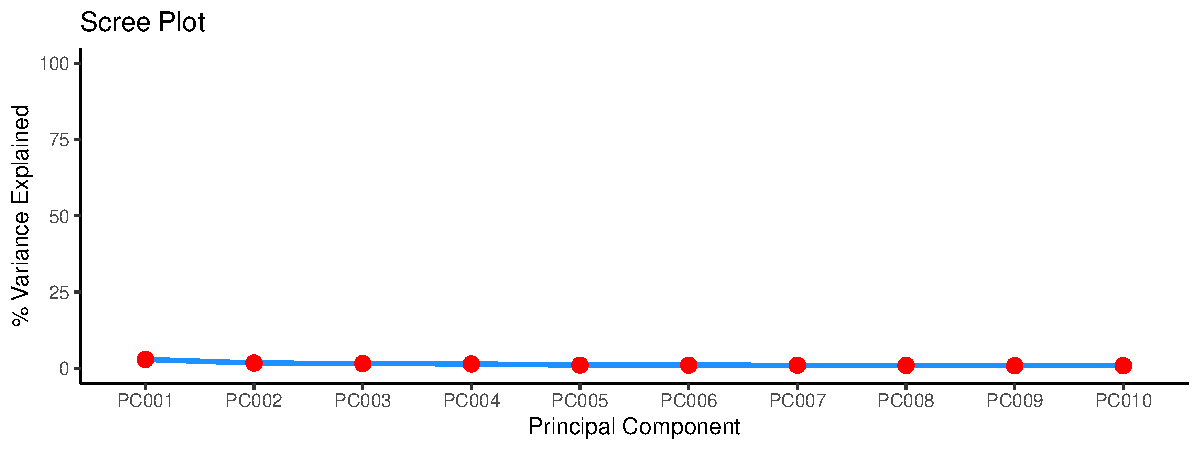
\includegraphics{_main_files/figure-latex/04_scree_plot-1.pdf}

In a Principal Component Analysis (PCA), the first three principal components may explain less than 15\% of the variance in the data if the data is highly dispersed or if there is a large amount of noise in the data. This means that the first three principal components are not capturing a significant portion of the variability in the data. This could be due to a lack of clear structure in the data or a lack of meaningful patterns that can be captured by the PCA. Alternatively, it could be due to the presence of many irrelevant features or variables in the data that are not contributing to the overall variance. This is one more of the reasons why GWPCA is more appropriate for STx data. Because, it may be true that the global PCs are not strong but locally this can change.

\hypertarget{identify-the-leading-genes-in-each-location}{%
\section{Identify the leading genes in each location}\label{identify-the-leading-genes-in-each-location}}

\begin{Shaded}
\begin{Highlighting}[]
\DocumentationTok{\#\# Extract leading genes}
\NormalTok{pcagw }\OtherTok{\textless{}{-}} \FunctionTok{gwpca\_LeadingGene}\NormalTok{(}\AttributeTok{gwpca =}\NormalTok{ pcagw, }
                           \AttributeTok{sfe =}\NormalTok{ sfe, }
                           \AttributeTok{pc\_nos =} \DecValTok{1}\SpecialCharTok{:}\DecValTok{4}\NormalTok{, }
                           \AttributeTok{type =} \StringTok{"single"}\NormalTok{, }
                           \AttributeTok{names =} \StringTok{"gene\_names"}\NormalTok{)}
\end{Highlighting}
\end{Shaded}

\begin{verbatim}
## 16  leading genes found for  PC1
## The leading genes in  PC1  are:
##     ADH1A        C7       CRP    CYP3A4      GLUL     GSTA2      HAMP      HBA2 
##         2        11         4       365         7         1        13        33 
##     IGLL5    MALAT1 MTRNR2L12  MTRNR2L8      NNMT     PTGDS      SAA1       SDS 
##        87        39       153       181        23        73        36       133 
## 21  leading genes found for  PC2
## The leading genes in  PC2  are:
##        C7       CAT     CFHR1       CRP    CYP3A4      GLUL      HBA2       HBB 
##         3         6        38        39       149        83         2        37 
##    IGFBP3    IGFBP7       IGJ     IGLL5    MALAT1 MTRNR2L10 MTRNR2L12  MTRNR2L8 
##        49        39        34       246        80        10        78       124 
##      NNMT      SAA1       SDS     TAGLN    UGT2B7 
##        42        12        69        20         1 
## 24  leading genes found for  PC3
## The leading genes in  PC3  are:
##     AEBP1        C7       CAT     CFHR1       CRP    CYP3A4      GLUL      HBA2 
##         2         2        27        20         5        20        17        27 
##       HBB    IGFBP3    IGFBP7       IGJ     IGLL5    MALAT1 MTRNR2L10 MTRNR2L12 
##       150        41        77         6       399       136         6        61 
##  MTRNR2L8      MYL9      NNMT      SAA1   SCGB3A1       SDS     TAGLN    UGT2B7 
##        25         9        24         6        56        15        26         4 
## 25  leading genes found for  PC4
## The leading genes in  PC4  are:
##     AEBP1       CAT     CFHR1       CRP     FXYD2      GLUL     GSTA2      HBA2 
##         1        53        15         7         7        33         3         2 
##       HBB    IGFBP3    IGFBP7       IGJ     IGLL5    MALAT1 MTRNR2L10 MTRNR2L12 
##       181       100        51        60       281       201         5        16 
##  MTRNR2L8      MYL9      NNMT      ORM2      SAA1       SDS    SPINK1     TAGLN 
##        16         5        55         6         6        37        12         4 
##    UGT2B7 
##         4
\end{verbatim}

\begin{Shaded}
\begin{Highlighting}[]
\NormalTok{pcagw }\OtherTok{\textless{}{-}} \FunctionTok{gwpca\_LeadingGene}\NormalTok{(}\AttributeTok{gwpca =}\NormalTok{ pcagw, }
                           \AttributeTok{sfe =}\NormalTok{ sfe, }
                           \AttributeTok{pc\_nos =} \DecValTok{1}\SpecialCharTok{:}\DecValTok{4}\NormalTok{, }
                           \AttributeTok{genes\_n =} \DecValTok{4}\NormalTok{, }
                           \AttributeTok{type =} \StringTok{"multi"}\NormalTok{, }
                           \AttributeTok{method =} \StringTok{"membership"}\NormalTok{, }
                           \AttributeTok{names =} \StringTok{"gene\_names"}\NormalTok{)}
\end{Highlighting}
\end{Shaded}

\begin{verbatim}
## The number of individual leading genes groups found for PC1 is: 110 
## These groups are: Too many to print them!
## The number of individual leading genes groups found for PC2 is: 240 
## These groups are: Too many to print them!
## The number of individual leading genes groups found for PC3 is: 310 
## These groups are: Too many to print them!
## The number of individual leading genes groups found for PC4 is: 421 
## These groups are: Too many to print them!
\end{verbatim}

\begin{Shaded}
\begin{Highlighting}[]
\DocumentationTok{\#\# Plot leading genes}
\FunctionTok{plotGWPCA\_leadingG}\NormalTok{(}\AttributeTok{gwpca =}\NormalTok{ pcagw,}
                   \AttributeTok{comps =} \DecValTok{1}\SpecialCharTok{:}\DecValTok{2}\NormalTok{,}
                   \AttributeTok{type =} \StringTok{"single"}\NormalTok{,}
                   \AttributeTok{arrange =} \ConstantTok{FALSE}\NormalTok{)}

\FunctionTok{plotGWPCA\_leadingG}\NormalTok{(}\AttributeTok{gwpca =}\NormalTok{ pcagw,}
                   \AttributeTok{comps =} \DecValTok{1}\NormalTok{,}
                   \AttributeTok{type =} \StringTok{"multi"}\NormalTok{,}
                   \AttributeTok{arrange =} \ConstantTok{FALSE}\NormalTok{)}
\end{Highlighting}
\end{Shaded}

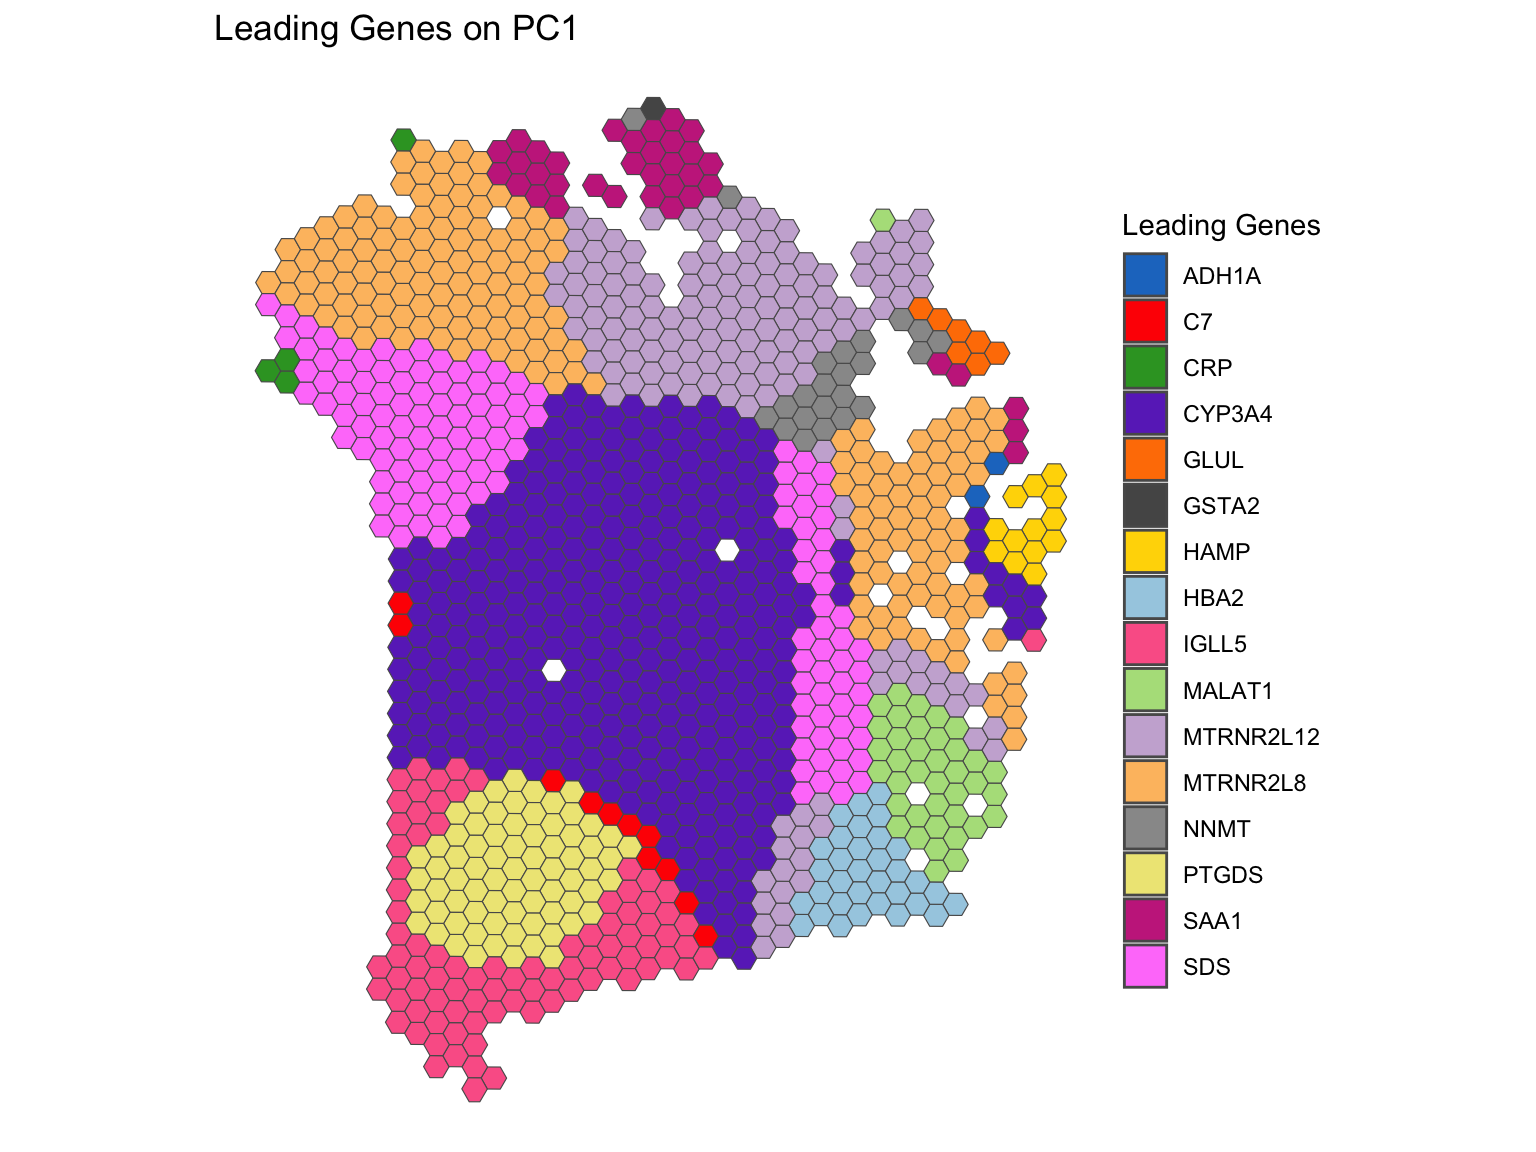
\includegraphics[width=0.33\linewidth]{_main_files/figure-latex/leading_genes2-1} 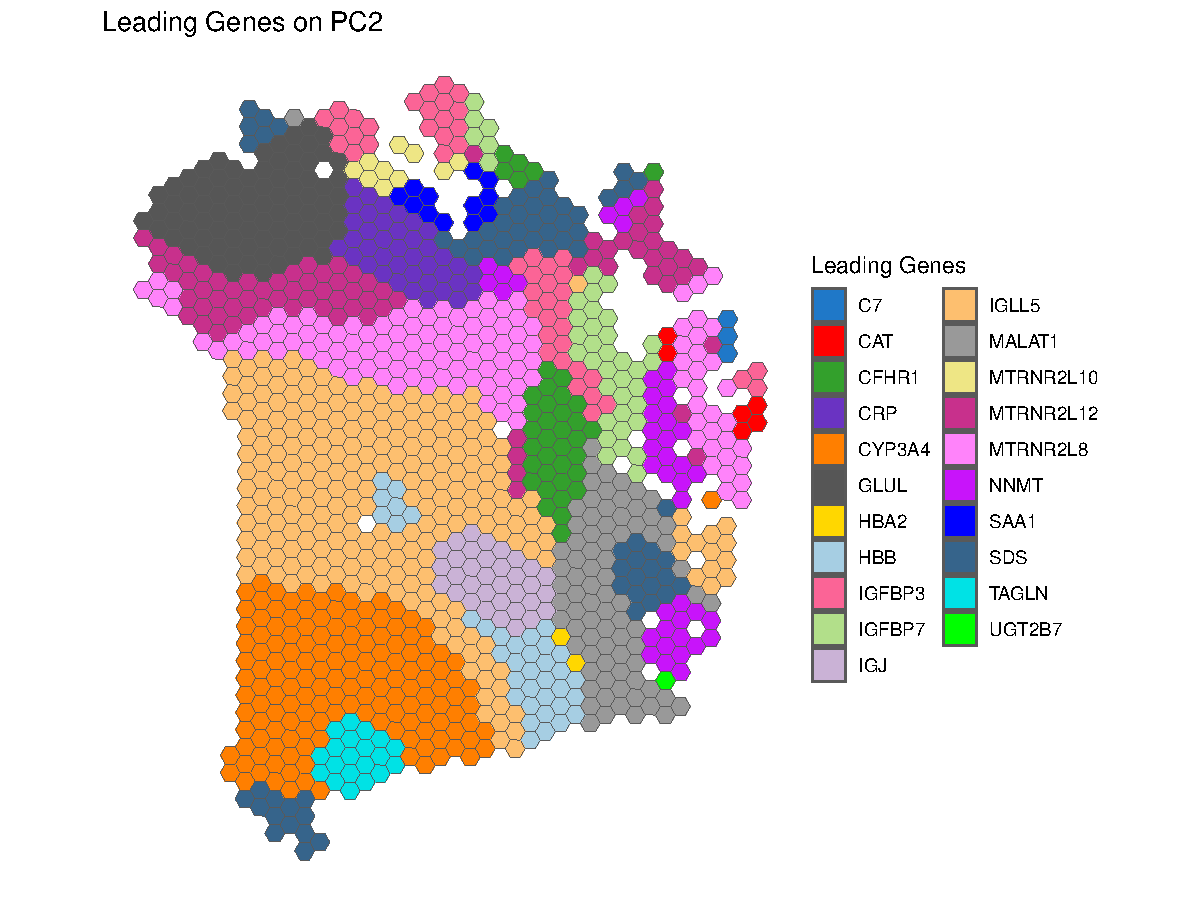
\includegraphics[width=0.33\linewidth]{_main_files/figure-latex/leading_genes2-2} \includegraphics[width=0.33\linewidth]{_main_files/figure-latex/leading_genes2-3}

\hypertarget{percentage-of-total-variation-ptv}{%
\section{Percentage of Total Variation (PTV)}\label{percentage-of-total-variation-ptv}}

Another useful diagnostic for PCA is the percentage of variability in the data explained by each of the components. This can be achieved by looking at the \texttt{var} component of \texttt{pcagw}; this is written as \texttt{pcagw\$var}. This is an XXXX by XX matrix - where XXXX is the number of observations and XX is the number of components. For each location, the XX columns correspond to the variance of each of the principal components. Looking at the proportion of each component in the sum of all of the variances shows how much of the variability in the data each component contributes. If, say, the first two components contributed 90\% of the total variance, then it is reasonable to assume that much of the variability in the data can be seen by just looking at these two components. Because this is geographically weighted PCA, however, this quantity varies across the map.

\begin{Shaded}
\begin{Highlighting}[]
\DocumentationTok{\#\# Calculate the PTV for multiple Components}
\NormalTok{pcagw }\OtherTok{\textless{}{-}} \FunctionTok{gwpca\_PropVar}\NormalTok{(}\AttributeTok{gwpca =}\NormalTok{ pcagw, }\AttributeTok{n\_comp =} \DecValTok{2}\SpecialCharTok{:}\DecValTok{10}\NormalTok{, }\AttributeTok{sfe =}\NormalTok{ sfe)}
\end{Highlighting}
\end{Shaded}

\begin{verbatim}
##     Comps_01         Comps_02        Comps_03        Comps_04    
##  Min.   : 6.279   Min.   :11.67   Min.   :16.43   Min.   :20.69  
##  1st Qu.: 9.483   1st Qu.:16.13   1st Qu.:21.24   1st Qu.:25.69  
##  Median :16.782   Median :25.54   Median :30.37   Median :34.46  
##  Mean   :17.370   Mean   :25.92   Mean   :31.35   Mean   :35.49  
##  3rd Qu.:22.534   3rd Qu.:32.87   3rd Qu.:39.42   3rd Qu.:43.81  
##  Max.   :38.254   Max.   :46.50   Max.   :54.25   Max.   :57.51  
##     Comps_05        Comps_06        Comps_07        Comps_08    
##  Min.   :24.64   Min.   :28.28   Min.   :31.49   Min.   :34.26  
##  1st Qu.:29.65   1st Qu.:33.13   1st Qu.:36.54   1st Qu.:39.53  
##  Median :37.79   Median :40.86   Median :43.53   Median :46.17  
##  Mean   :38.98   Mean   :42.07   Mean   :44.84   Mean   :47.38  
##  3rd Qu.:47.17   3rd Qu.:49.78   3rd Qu.:52.16   3rd Qu.:54.19  
##  Max.   :60.60   Max.   :62.97   Max.   :65.04   Max.   :67.03  
##     Comps_09        Comps_10    
##  Min.   :36.76   Min.   :39.15  
##  1st Qu.:42.34   1st Qu.:45.05  
##  Median :48.60   Median :50.96  
##  Mean   :49.73   Mean   :51.91  
##  3rd Qu.:56.07   3rd Qu.:57.77  
##  Max.   :68.83   Max.   :70.39
\end{verbatim}

\begin{Shaded}
\begin{Highlighting}[]
\DocumentationTok{\#\# Plot PTV}
\FunctionTok{plotGWPCA\_ptv}\NormalTok{(}\AttributeTok{gwpca =}\NormalTok{ pcagw,}
              \AttributeTok{comps =} \DecValTok{1}\SpecialCharTok{:}\DecValTok{10}\NormalTok{,}
              \AttributeTok{type =} \StringTok{"violin"}\NormalTok{)}

\DocumentationTok{\#\# Map PTV}
\FunctionTok{plotGWPCA\_ptv}\NormalTok{(}\AttributeTok{gwpca =}\NormalTok{ pcagw,}
              \AttributeTok{comps =} \DecValTok{1}\SpecialCharTok{:}\DecValTok{6}\NormalTok{,}
              \AttributeTok{type =} \StringTok{"map"}\NormalTok{)}
\end{Highlighting}
\end{Shaded}

\includegraphics{_main_files/figure-latex/04_ptv-1.pdf} \includegraphics{_main_files/figure-latex/04_ptv-2.pdf}

\hypertarget{identify-discrepancies}{%
\section{Identify discrepancies}\label{identify-discrepancies}}

Global PCA can be used to identify multivariate outliers. Extending this, it is also possible to use local PCA (i.e., GWPCA) to identify local outliers. One way of doing this links back to the cross-validation idea used earlier to select a bandwidth. Recall that this is based on a score of how well each observation can be reconstructed on the basis of local PCs. The score measures the total discrepancies of true data values from the reconstructed ones - and the bandwidth chosen is the one minimising this. However, the total discrepancy score is the sum of the individual discrepancies. A very large individual discrepancy associated with an observation suggests it is very different - in a multidimensional way, to the observations near to it. These discrepancies can be calculated with the \texttt{gwpca.cv.contrib} function.

\begin{Shaded}
\begin{Highlighting}[]
\DocumentationTok{\#\# Plot the discrepancies as boxplot}
\FunctionTok{plotGWPCA\_discr}\NormalTok{(pcagw, }\AttributeTok{type =} \StringTok{"box"}\NormalTok{)}
\end{Highlighting}
\end{Shaded}

\includegraphics{_main_files/figure-latex/04_discrep1-1.pdf}

\begin{Shaded}
\begin{Highlighting}[]
\DocumentationTok{\#\# Plot the discrepancies map}
\FunctionTok{plotGWPCA\_discr}\NormalTok{(pcagw, }\AttributeTok{type =} \StringTok{"map"}\NormalTok{)}
\end{Highlighting}
\end{Shaded}

\includegraphics{_main_files/figure-latex/04_discrep2-1.pdf}

Comment on the discrepancies and the Liver histopathology

\begin{Shaded}
\begin{Highlighting}[]
\DocumentationTok{\#\# Get location data for the discrepancies}
\NormalTok{discrepancy\_loc\_dt }\OtherTok{\textless{}{-}} \FunctionTok{getDiscrepancyLocData}\NormalTok{(}\AttributeTok{sfe =}\NormalTok{ sfe, }
                                            \AttributeTok{gwpca =}\NormalTok{ pcagw, }
                                            \AttributeTok{sample\_id =} \StringTok{"JBO019"}\NormalTok{)}
\end{Highlighting}
\end{Shaded}

Another possibility to understand the nature of the outlier is a parallel coordinates heatmap. Here, each observation neighbouring the location that has been found to be an outlier is shown as a column with the genes in rows. Since here we are investigating local outliers, one particular observation is highlighted in red -the outlier-, and the remaining ones in grey, but with the intensity of the grey fading according to their distance from the red observation. This enables you to see what characteristic the red observation has that means it as outlying from its neighbours. The plot can be created using \texttt{gw.pcplot}:

\begin{Shaded}
\begin{Highlighting}[]
\FunctionTok{head}\NormalTok{(discrepancy\_loc\_dt)}
\end{Highlighting}
\end{Shaded}

\begin{verbatim}
##                              barcodes coords.pxl_col_in_fullres
## AAGTGCCTTGACTGTA-1 AAGTGCCTTGACTGTA-1                     11086
## ACCCGGATGACGCATC-1 ACCCGGATGACGCATC-1                      9908
## ACCTCCGTTATTCACC-1 ACCTCCGTTATTCACC-1                      9113
## AGATGATGGAGTCTGG-1 AGATGATGGAGTCTGG-1                      9117
## AGGTATAATTGATAGT-1 AGGTATAATTGATAGT-1                      9312
## AGTGAACAAACTTCTC-1 AGTGAACAAACTTCTC-1                     11088
##                    coords.pxl_row_in_fullres discScore
## AAGTGCCTTGACTGTA-1                      5148  22793.56
## ACCCGGATGACGCATC-1                      5607  24165.26
## ACCTCCGTTATTCACC-1                      4255  27035.77
## AGATGATGGAGTCTGG-1                      4933  27423.00
## AGGTATAATTGATAGT-1                      4593  23839.25
## AGTGAACAAACTTCTC-1                      5374  25111.79
##                                          geometry
## AAGTGCCTTGACTGTA-1 POLYGON ((11020.03 5034.788...
## ACCCGGATGACGCATC-1 POLYGON ((9841.741 5494.291...
## ACCTCCGTTATTCACC-1 POLYGON ((9046.741 4142.291...
## AGATGATGGAGTCTGG-1 POLYGON ((9050.741 4820.291...
## AGGTATAATTGATAGT-1 POLYGON ((9245.076 4480.294...
## AGTGAACAAACTTCTC-1 POLYGON ((11020.91 5261.585...
\end{verbatim}

\begin{Shaded}
\begin{Highlighting}[]
\NormalTok{focus }\OtherTok{\textless{}{-}}\NormalTok{ discrepancy\_loc\_dt}\SpecialCharTok{$}\NormalTok{barcodes[}\DecValTok{1}\SpecialCharTok{:}\DecValTok{2}\NormalTok{]}
\NormalTok{bw }\OtherTok{=} \DecValTok{3}\SpecialCharTok{*}\NormalTok{sfe}\SpecialCharTok{@}\NormalTok{metadata[[}\StringTok{"spotDiameter"}\NormalTok{]][[}\StringTok{"JBO019"}\NormalTok{]][[}\StringTok{"spot\_diameter\_fullres"}\NormalTok{]]}

\CommentTok{\# Plot the heatmap to visualise the genes that make this location an outlier}
\FunctionTok{plotGWPCA\_discrHeatmap}\NormalTok{(}\AttributeTok{sfe =}\NormalTok{ sfe,}
                       \AttributeTok{assay =} \StringTok{"logcounts"}\NormalTok{,}
                       \AttributeTok{vars =} \ConstantTok{NULL}\NormalTok{,}
                       \AttributeTok{focus =}\NormalTok{ focus,}
                       \AttributeTok{dMetric =} \StringTok{"euclidean"}\NormalTok{, }
                       \AttributeTok{sample\_id =} \StringTok{"JBO019"}\NormalTok{,}
                       \AttributeTok{bw =}\NormalTok{ bw, }
                       \AttributeTok{mean.diff =} \DecValTok{1}\NormalTok{, }
                       \AttributeTok{show.vars =} \StringTok{"top"}\NormalTok{, }
                       \AttributeTok{scale =} \StringTok{"row"}\NormalTok{, }
                       \AttributeTok{gene.names =} \ConstantTok{TRUE}\NormalTok{,}
                       \AttributeTok{color =} \FunctionTok{rev}\NormalTok{(}\FunctionTok{colorRampPalette}\NormalTok{(}\FunctionTok{brewer.pal}\NormalTok{(}\DecValTok{11}\NormalTok{, }\StringTok{"RdBu"}\NormalTok{))(}\DecValTok{1000}\NormalTok{)))}
\end{Highlighting}
\end{Shaded}

\includegraphics{_main_files/figure-latex/04_discrep4-1.pdf} \includegraphics{_main_files/figure-latex/04_discrep4-2.pdf}

\begin{Shaded}
\begin{Highlighting}[]
\NormalTok{discrepancy\_gene\_dt }\OtherTok{\textless{}{-}} \FunctionTok{getDiscrepancyGeneData}\NormalTok{(}\AttributeTok{sfe =}\NormalTok{ sfe,}
                                              \AttributeTok{assay =} \StringTok{"logcounts"}\NormalTok{,}
                                              \AttributeTok{vars =} \ConstantTok{NULL}\NormalTok{,}
                                              \AttributeTok{focus =}\NormalTok{ focus[}\DecValTok{2}\NormalTok{],}
                                              \AttributeTok{dMetric =} \StringTok{"euclidean"}\NormalTok{, }
                                              \AttributeTok{sample\_id =} \StringTok{"JBO019"}\NormalTok{,}
                                              \AttributeTok{bw =}\NormalTok{ bw, }
                                              \AttributeTok{mean.diff =} \DecValTok{1}\NormalTok{, }
                                              \AttributeTok{show.vars =} \StringTok{"top"}\NormalTok{,}
                                              \AttributeTok{exportExpression =} \ConstantTok{TRUE}\NormalTok{)}
\FunctionTok{head}\NormalTok{(discrepancy\_gene\_dt)}
\end{Highlighting}
\end{Shaded}

\begin{verbatim}
##                 AACCCTACTGTCAATA-1 ACATGGCGCCAAAGTA-1 ACCCGGATGACGCATC-1
## ENSG00000078808          1.9800764          1.7845077           0.000000
## ENSG00000157916          1.1230410          2.3434121           0.000000
## ENSG00000171603          0.6681445          0.8599719           1.667949
## ENSG00000162496          1.1230410          0.8599719           0.000000
## ENSG00000074964          1.4683664          0.0000000           1.964768
## ENSG00000158828          1.1230410          0.8599719           0.000000
##                 ACGATCATCTTGTAAA-1 AGGGTCGATGCGAACT-1 ATAGTTCCACCCACTC-1
## ENSG00000078808           1.434549          0.0000000          0.0000000
## ENSG00000157916           1.094451          1.1491034          0.7197148
## ENSG00000171603           0.000000          0.0000000          0.0000000
## ENSG00000162496           1.094451          2.2182483          1.5560955
## ENSG00000074964           1.709571          0.6860569          0.7197148
## ENSG00000158828           1.434549          2.0159260          1.1976848
##                 ATATCAACCTACAGAG-1 CATCTTACACCACCTC-1 CCATCTCACCAGTGAA-1
## ENSG00000078808           1.848204           2.383137          0.7918769
## ENSG00000157916           1.356318           1.489110          2.2192853
## ENSG00000171603           0.000000           0.000000          1.3002121
## ENSG00000162496           2.214350           0.000000          2.2192853
## ENSG00000074964           1.028715           1.140629          0.7918769
## ENSG00000158828           2.632509           1.140629          0.7918769
##                 CCGATCTCAACCTTAT-1 CGCACGTGCGCTATCA-1 CGCTAGAGACCGCTGC-1
## ENSG00000078808          1.1456336          2.0109592           1.070644
## ENSG00000157916          1.7760473          2.4713829           1.070644
## ENSG00000171603          0.0000000          0.0000000           0.000000
## ENSG00000162496          0.6836662          1.7105588           1.678406
## ENSG00000074964          1.1456336          0.8136275           1.070644
## ENSG00000158828          0.6836662          1.3307021           1.070644
##                 CTAGGTCTGAAGGAAT-1 GAAAGAACAGCGTTAT-1 GCAGACCCAGCACGTA-1
## ENSG00000078808          1.1275395          2.0533150          2.1052992
## ENSG00000157916          0.0000000          1.5312450          0.8684635
## ENSG00000171603          0.6712291          0.7049757          0.0000000
## ENSG00000162496          1.1275395          2.5947724          1.4067734
## ENSG00000074964          1.4736763          1.5312450          1.4067734
## ENSG00000158828          1.1275395          1.5312450          0.8684635
##                 GCGCAAGAGCGCGCTG-1 GCTCGCTCATGTCCAA-1 GCTGTTGCTACCGAAC-1
## ENSG00000078808           2.505794          1.4756527           2.004239
## ENSG00000157916           1.117631          1.8764253           1.588731
## ENSG00000171603           0.000000          0.0000000           1.325320
## ENSG00000162496           2.173035          2.1897262           1.588731
## ENSG00000074964           0.000000          0.9188039           1.002827
## ENSG00000158828           1.739765          0.9188039           1.811392
##                 GGTTCTACTCGTCTGA-1 GTGCGACAGGGAGTGT-1 TAGACTACCTAGCGTT-1
## ENSG00000078808          1.7977169           1.633005           1.421361
## ENSG00000157916          1.4066078           1.633005           0.000000
## ENSG00000171603          0.8683433           0.000000           0.000000
## ENSG00000162496          2.3583475           1.263669           2.123256
## ENSG00000074964          0.8683433           2.170771           0.000000
## ENSG00000158828          1.4066078           1.633005           1.695032
##                 TAGGGAGCTTGGGATG-1 TATAGATGGTCGCAGT-1 TATATCCCTGGGAGGA-1
## ENSG00000078808          2.2316954          0.0000000          0.7102708
## ENSG00000157916          0.7985659          1.9335702          2.6061791
## ENSG00000171603          0.0000000          0.0000000          0.0000000
## ENSG00000162496          0.7985659          1.9335702          1.1841040
## ENSG00000074964          0.7985659          0.9560551          0.7102708
## ENSG00000158828          0.0000000          1.5260667          1.1841040
##                 TATTACCATCCTGCTT-1 TCATTTAAGTCTCCGA-1 TCTGGGAACCTTTGAA-1
## ENSG00000078808          1.9382158          2.1150669          2.3926955
## ENSG00000157916          1.0928336          1.2220876          1.4967274
## ENSG00000171603          0.6475105          0.0000000          0.6846746
## ENSG00000162496          2.4677235          1.5846069          2.0131754
## ENSG00000074964          0.6475105          1.2220876          0.6846746
## ENSG00000158828          1.0928336          0.7367522          1.4967274
##                 TGACATCGAGCGGACC-1 TGACGATGCACTAGAA-1 TTGAATTCACGTGAGG-1
## ENSG00000078808          1.9076262          2.4843308          1.8133018
## ENSG00000157916          1.2485083          1.3402294          2.0507006
## ENSG00000171603          0.7552962          1.0152672          0.0000000
## ENSG00000162496          2.7012885          1.3402294          2.0507006
## ENSG00000074964          1.2485083          0.5951586          0.7036449
## ENSG00000158828          1.6153854          0.0000000          1.1745524
##                 TTGACGCTCCATGAGC-1 gene_name
## ENSG00000078808           2.296259      SDF4
## ENSG00000157916           1.851153      RER1
## ENSG00000171603           0.000000    CLSTN1
## ENSG00000162496           1.851153     DHRS3
## ENSG00000074964           0.000000 ARHGEF10L
## ENSG00000158828           1.851153     PINK1
\end{verbatim}

  \bibliography{book.bib,packages.bib}

\end{document}
